% !TEX program = xelatex
\documentclass{diploma_style}

\usepackage[hyperref=true,
            backref=true,
            style=numeric-comp,
            sorting=none,
            maxnames=11,
            giveninits=false,
            url=false,
            isbn=false,
            defernumbers=true
            ]{biblatex}

\renewbibmacro{in:}{}
\AtEveryBibitem{%
    \clearlist{language}%
}

\addbibresource{sajat.bib}
\addbibresource{EMBL.bib}
\addbibresource{mouse.bib}

\DeclareRefcontext{journal}{labelprefix=J}

\DeclareBibliographyCategory{journal}
\addtocategory{journal}{balazs_real-time_2017,de_medeiros_light-sheet_2016,strnad_inverted_2016,hoyer_breaking_2016}

%\DeclareRefcontext{others}{labelprefix=J}

\DeclareBibliographyCategory{others}
\addtocategory{others}{jakus_genetic_2010,gyorffy_recurrenceonline:_2011,shi_combined_2014}


\DeclareRefcontext{conference}{labelprefix=C}
\DeclareBibliographyCategory{conference}
\addtocategory{conference}{balazs_gpu-based_2016,balazs_gpu-based_2016-1,balazs_gpu-based_2017}

\defbibheading{secbib}[\bibname]{
\section*{#1}
\markboth{#1}{#1}}



\setacronymstyle{long-short}

\newacronym{spim}{SPIM}{single plane illumination microscopy}
\newacronym{lsfm}{LSFM}{light-sheet fluorescence microscopy}
\newacronym{smlm}{SMLM}{single molecule localization microscopy}
\newacronym{gfp}{GFP}{green fluorescent protein}
\newacronym{pdf}{PSF}{point spread function}
\newacronym{otf}{OTF}{optical transfer function}
\newacronym{opfos}{OPFOS}{orthogonal plane fluorescent optical sectioning}
\newacronym{muvi}{MuVi-SPIM}{Multiview SPIM}
\newacronym{dslm}{DSLM}{digitally scanned light-sheet microscopy}
\newacronym{dct}{DCT}{discrete cosine transform}
\newacronym{dft}{DFT}{discrete fourier transform}
\newacronym{dwt}{DWT}{discrete wavelet transform}
\newacronym{fov}{FOV}{field of view}
\newacronym{fn}{FN}{field number}
\newacronym{roi}{ROI}{region of interest}
\newacronym{2d}{2D}{two-dimensional}
\newacronym{3d}{3D}{three-dimensional}
\newacronym{na}{NA}{numerical aperture}
\newacronym{miam}{MIAM}{multi-imaging axis microscopy}
\newacronym{clsm}{CLSM}{confocal laser scanning microscopy}
\newacronym{tlsm}{TLSM}{thin light-sheet microscopy}
% \newacronym{EMBL}{EMBL}{European Molecular Biology Laboratory}
\newacronym{sted}{STED}{Stimulated Emission Depletion}
\newacronym{resolft}{RESOLFT}{reversible saturable optical fluorescence transitions}
\newacronym{ccd}{CCD}{charge coupled device}
\newacronym{emccd}{EM-CCD}{electron multiplying CCD}
\newacronym{scmos}{sCMOS}{scientific CMOS}
\newacronym{smos}{CMOS}{complementary metal oxide semiconductor}
\newacronym{te}{TE}{trophoectoderm}
\newacronym{icm}{ICM}{inner cell mass}
\newacronym{fep}{FEP}{fluorinated ethylene propylene}
\newacronym{peek}{PEEK}{polyether ether ketone}
\newacronym{jpeg}{JPEG}{joint photographic experts group}
\newacronym{hevc}{HEVC}{high efficiency video codec}
\newacronym{dpcm}{DPCM}{differential pulse code modulation}
\newacronym{fwhm}{FWHM}{full width at half maximum}
\newacronym{bfp}{BFP}{back focal plane}
\newacronym{fpga}{FPGA}{field programmable gate array}
\newacronym{fps}{fps}{frames per second}
\newacronym{yfp}{YFP}{yellow fluorescent protein}
\newacronym{gpu}{GPU}{graphics processing unit}
\newacronym{cpu}{CPU}{central processing unit}
\newacronym{ecsd}{eCSD}{electronic confocal slit detection}
\newacronym{wnl}{WNL}{within noise level}
\newacronym{dstorm}{dSTORM}{direct stochastic optical reconstruction microscopy}
\newacronym{snr}{SNR}{signal-to-noise ratio}

\def\b3d{B\textsuperscript{3}D}
\newcommand{\etal}{\textit{et al.}\xspace}

\DeclareMathOperator{\na}{NA}
\DeclareMathOperator{\NA}{NA}
\DeclareMathOperator{\pred}{Pred}
\DeclareMathOperator{\Pred}{Pred}

\author{\href{mailto:balint.balazs@embl.de}{Bálint Balázs}}
\supervisor{\href{mailto:rozsabal@koki.hu}{Balázs Rózsa, \textit{M.D., Ph.D.}}}
\lab{\href{http://www.embl.de/}{European Molecular Biology Laboratory}}
\university{\href{http://www.ppke.hu/}{Pázmány Péter Catholic University}}
\collegeordept{\href{http://www.itk.ppke.hu/}{Faculty of Information Technology and Bionics \\ Roska Tamás Doctoral School of Sciences and Technology}}
\degreedate{A thesis submitted for the degree of \\ \textit{Doctor of Philosophy} \\ 2017}
\ppkelogo{
\includegraphics[width=3cm]{figures/0_front/ITK_logo}}
\degree{PhD}

\makeglossaries

\title{A new angle on light-sheet microscopy and real-time image processing}
%\date{2012 november}



\hyphenation{CameraLink}



\begin{document}

\pagestyle{plain}

\maketitle
\pagenumbering{roman}



% !TEX root = dissertation_BB.tex
%% spellcheck-language en-US

\chapter*{Abstract}
\addcontentsline{toc}{chapter}{Abstract}
Light-sheet fluorescence microscopy, also called single plane illumination microscopy, has numerously proven its usefulness for long term imaging of embryonic development. This thesis tackles two challenges of light-sheet microscopy: high resolution isotropic imaging of delicate, light-sensitive samples, and real-time image processing and compression of light-sheet microscopy images.

A symmetric light-sheet microscope is presented, featuring two high numerical aperture objectives arranged in \SI{120}{\degree}, both capable of illuminating the sample and detecting the fluorescence signal. It allows for multi-view imaging of delicate samples where rotation is not possible. The optical properties of the microscope are characterized, and its imaging capabilities are demonstrated on \textit{Drosophila melanogaster} embryos and mouse zygotes.

To address the big data problem of light-sheet microscopy, a real-time, GPU-based image processing pipeline is presented.
Alongside its capability of performing commonly required preprocessing tasks, such as image fusion of opposing views, immediately during image acquisition, it also contains a novel, high-speed image compression method. This algorithm is suitable for both a lossless and a noise-dependent lossy image compression, the latter allowing for a significantly increased compression ratio, without affecting the results of any further analysis.
A detailed performance analysis is presented of the different compression modes for various biological samples and imaging modalities.


% preprocessing and compressing the data real-time
%   parallel processing, GPU
%   reduce time for evaluation
%   reduce necessary storage and costs
%   noise dependent lossy compression
%   within noise level compression - although not lossless in the mathematical sense, but the introduced differences for each pixel are within the range of uncertainty of the measurement

% % "Fluorescence imaging techniques such as single molecule localization microscopy, high-content screening and light-sheet microscopy are producing ever-larger datasets, which poses increasing challenges in data handling and data sharing. Here, we introduce
% A real-time compression library is introduced that allows for very fast (beyond 1 GB/s) compression and decompression of microscopy datasets during acquisition. In addition to an efficient lossless mode, the algorithm also includes a lossy option, which limits pixel deviations to the intrinsic noise level of the image and yields compression ratio of up to 100-fold. A detailed performance analysis is presented of the different compression modes for various biological samples and imaging modalities.




% spellchecker:disable
\chapter*{Tartlami kivonat}
\addcontentsline{toc}{chapter}{Tartlami kivonat}
Absztrakt magyarul.
% spellchecker: enable

\addtocontents{toc}{\protect{\pdfbookmark[0]{\contentsname}{toc}}}
\tableofcontents
\pagestyle{fancy}
\markboth{\MakeUppercase{Contents}}{}


\listoffigures
\addcontentsline{toc}{chapter}{List of Figures}

\listoftables
\addcontentsline{toc}{chapter}{List of Tables}

\glsaddall[types={\acronymtype}]
\printglossary[type=\acronymtype, title=List of Abbreviations, toctitle=List of Abbreviations]



\cleardoublepage
\setcounter{page}{1}
\pagenumbering{arabic}

\chapter*{Introduction}
\markboth{\MakeUppercase{Introduction}}{}
\addcontentsline{toc}{chapter}{Introduction}
% !TEX root = dissertation_BB.tex
%% spellcheck-language en-US

%   ###
%  #  ##
%  # # #
%  ##  #
%   ###

\chapter*{Introduction}
\setcounter{page}{1}
\pagenumbering{arabic}
\markboth{\MakeUppercase{Introduction}}{}
\addcontentsline{toc}{chapter}{Introduction}


% Hooke's Micrographia 1665 \cite{hooke_micrographia:_1665}
Coming soon.
\cleardoublepage

% !TEX root = dissertation_BB.tex
%% spellcheck-language en-US

%   #
%  ##
%   #
%   #
%  ###

\chapter{Live imaging in three dimensions}
\label{ch:intro}

\graphicspath{{./figures/1_spim/}}


Live imaging is indispensable to understand the processes during embryonic development. In an ideal setting, the ultimate microscope would be able to record a continuos, three dimensional (3D), multicolor dataset of any biological process of interest with the highest possible resolution. Due to several limitations in physics and biology this is not possible. Therefore, a compromise is necessary. The diffractive nature of light, the lifetime of fluorescent probes and the photosensitivity of biological specimens all require microscopy to be able to adapt to answer the question at hand. In order to acquire useful data one has to choose a tradeoff between spatial and temporal resolution and signal contrast, while making sure the biology is not affected by the imaging process itself (\autoref{fig:tradeoffs}) \cite{laissue_assessing_2017}.

\begin{figure}[bht]
  \centering
  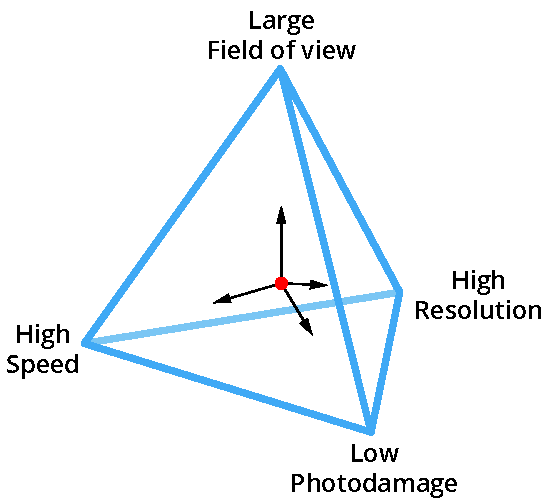
\includegraphics[width=0.4\textwidth]{tradeoffs}
  \bcaption[Tradeoffs in fluorescence microscopy for live imaging]{Also called the ``pyramid of frustration". When optimizing the imaging conditions (red dot), a tradeoff has to be made between resolution, contrast, and imaging speed, while avoiding photodamage. One can only be improved at the expense of the others due to the limited photon budget of the fluorescent molecules. Adapted from \cite{laissue_assessing_2017}.}
  \label{fig:tradeoffs}
\end{figure}


% Light microscopy is one of the oldest methods that is still widely used today to investigate the inner workings of microscopic life. A particularly important branch is fluorescence microscopy \cite{diaspro_optical_2011}, that relies on using fluorescent labels that mark specific structures inside the specimens. 

\section{Wide-field fluorescence microscopy}

Fluorescence microscopy \cite{lichtman_fluorescence_2005,diaspro_optical_2011}, as a subset of light microscopy, is one of the few methods that allow subcellular imaging of live specimens. The first use of the term fluorescence is credited to  George Gabriel Stokes \cite{stokes_change_1852}, and it refers to the phenomenon of light emission following the absorption of light or other electromagnetic radiation. As the name of the technique suggests, this method collects fluorescent light from the specimens.
% which has numerous advantages, but also some drawbacks.
Since biological tissues are usually not fluorescent, except for some autofluorescence mostly at shorter wavelengths, fluorescent dyes or proteins have to be introduced to the system in order to be able to collect the necessary information. The advantage of this is that the signal of the labeled structures will be of very high ratio compared to the background.

A fluorescent molecule is capable of absorbing photons in a given wavelength range (excitation spectrum) and temporarily store its energy by having an electron in a higher energy state, \textit{i.e.}, in an excited state. This excited state, however, is not stable, and the electron quickly returns to the ground state while emitting a photon with equal energy to the energy difference between the excited and ground states. The energy of the absorbed and emitted photons are not the same, as energy loss occurs due to internal relaxation events, and the emitted photon has lower energy than the absorbed photon. This phenomenon is called the Stokes shift, or red shift, and can be exploited in microscopy to drastically increase the signal to noise ratio by filtering out the illumination light (\autoref{fig:spectrum}).

  \begin{figure}
    \centering
    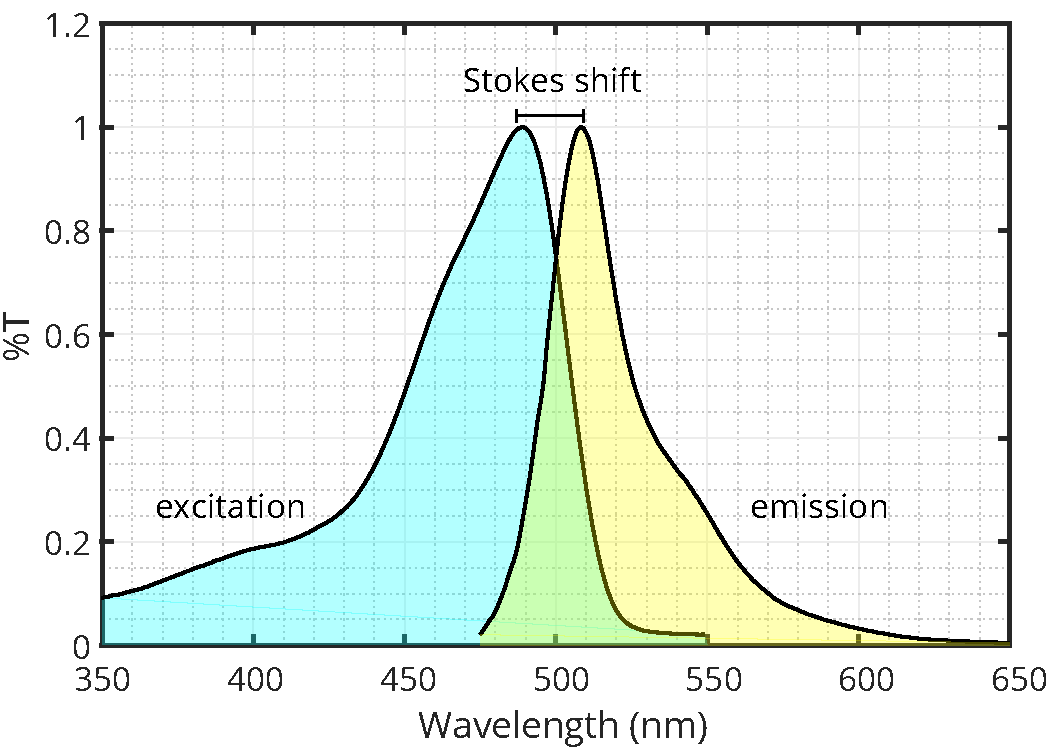
\includegraphics[width=0.6\textwidth]{spectrum/egfp}
    \bcaption[Excitation and emission spectrum of enhanced green fluorescent protein (EGFP)]{Excitation spectrum in blue, emission spectrum in yellow. The separation between the two spectra is due to the Stokes shift, which is 19 nm for EGFP. Emission and excitation light can be separated by a long-pass filter at \SI{500}{nm}. Data from \cite{noauthor_spectra_nodate}.}
    \label{fig:spectrum}
  \end{figure}

  % Although this process can disturb the natural environment 

  %  very small amount of illumination photons will result in fluorescence ($<0.0001\%$), the signal to noise ratio of the fluorescence is still very high due to the filtering.

  \subsection{Fluorescent proteins}
    Traditionally, synthetic fluorescent dyes were used to label certain structures in the specimens. Some of these directly bind to their target,
    % such as DAPI to DNA,
    and others can be used when conjugated to an antibody specific to the structure of interest. A requirement for these methods is that the fluorescent label has to be added to the sample from an external source, and, in many cases, this also necessitates sample preparation techniques incompatible with live imaging, such as fixation \cite{bacallao_guiding_1990}.

    The discovery of fluorescent proteins has revolutionized fluorescence microscopy. Since these molecules are proteins, they can be produced directly by the organism if the proper genetic modifications are performed. Even though this was a hurdle at the time of discovering the green fluorescent protein (GFP) \cite{shimomura_extraction_1962}, genetic engineering techniques evolved since then \cite{prasher_primary_1992}, and not only has its gene been successfully integrated in the genome of a multitude of organisms \cite{chalfie_green_1994,amsterdam_aequorea_1995,okabe_green_1997}, but many variants have been also engineered by introducing mutations to increase fluorescence intensity, and to change the fluorescence spectrum to allow multicolor imaging \cite{heim_wavelength_1994,heim_engineering_1996,cormack_facs-optimized_1996,okabe_green_1997}. The usefulness and impact of these proteins are so profound, that in 2008 the Nobel Prize in chemistry was awarded to Osamu Shimomura, Martin Chalfie, and Roger Tsien ``for the discovery and development of the green fluorescent protein, GFP" \cite{service_three_2008}.


  \subsection{Wide-field image formation}
    By imaging fluorescently labelled specimens, a wide-field fluorescence microscope has the capability of discriminating illumination light from emitted fluorescent light due to the Stokes shift described in the previous section. The microscope's operating principle is depicted in \autoref{fig:wide-field}.

    Light from a source, typically a mercury lamp is focused on the back focal plane of the objective to create even illumination of the sample. Before entering the objective, the light is filtered, so only the wavelengths that correspond to the excitation properties of the observed fluorophores are transmitted. Since the same objective is used for both illumination and detection, a dichroic mirror is utilized to decouple the illumination and detection paths. The emitted light is filtered again to make sure any reflected and scattered light from the illumination source is blocked to increase signal to noise ratio.
    Finally, light is focused by a tube lens to create a magnified image on the camera sensor.
    
    This type of arrangement is called infinity-corrected optics, since the back focal point of the objective is in ``infinity", meaning that the light exiting the back aperture is parallel. This is achieved by placing the sample exactly at the focal point of the objective. Infinity-corrected optics have the advantage that they allow placing various additional optical elements in the infinity space (\textit{i.e.}, the space between the objective and the tube lens) without affecting the image quality. In this example such elements are the dichroic mirror and the emission filter. 

    \begin{figure}[tb]
      \centering
      \includegraphics[page=4,width=0.7\textwidth]{spim_cyl}
      \bcaption[Wide-field fluorescence microscope]{The light source is focused on the back focal plane of the objective to provide an even illumination to the sample. Emitted photons are collected by the objective, and are separated from the illumination light by a dichroic mirror. Inset: Light collection of an objective lens. $\alpha$: light collection half-angle; $f$: focal length; $r$: radius of lens.}
      \label{fig:wide-field}
    \end{figure}


    The combination of the objective and tube lens together will determine the magnification of the system, it will be the ratio of the focal lengths of these lenses:
    \begin{equation}
      M = \frac{f_{TL}}{f_{OBJ}}.
      \label{eq:magnification}
    \end{equation}
    The final field of view (FOV) of the microscope will depend on the magnification, and also on the size of the imaging sensor ($D$), and the objective field number ($FN$):
    \begin{equation}
      FOV = \frac{\min(D, FN)}{M}.
      \label{eq:FOV}
    \end{equation}

    Apart from the magnification, the most important property of the objective is the half-angle of the light acceptance cone, $\alpha$ (\autoref{fig:wide-field}, inset). This not only determines the amount of collected light, but also the achievable resolution of the system (see \autoref{sec:resolution}). This angle depends on the size of the lens relative to its focal length. In other words it depends on the aperture of the lens, which is why the expression \textit{numerical aperture} (NA) is more commonly used to express this property of the objective:
    \begin{equation}
      \text{NA} = n\cdot \sin \alpha.
      \label{eq:NA}
    \end{equation}

    For small $\alpha$ angles, the following approximation holds true: $\sin \alpha \approx \tan \alpha \approx \alpha$. Thus, the numerical aperture can also be expressed as a ratio of the radius of the lens and the focal length:
    \begin{equation}
      NA \approx n \frac{r}{f},\quad \text{when }\alpha \ll 1.
    \end{equation}
    % This expression also shows the relationship of the numerical aperture and the f-number commonly used in photography to characterize a lens' aperture:
    % \begin{equation}
    %     f\# = \frac{f}{d} \approx \frac{2}{n\cdot NA}
    % \end{equation}


    % ########  ########  ######  
    % ##     ## ##       ##    ## 
    % ##     ## ##       ##       
    % ########  ######    ######  
    % ##   ##   ##             ## 
    % ##    ##  ##       ##    ## 
    % ##     ## ########  ######  

  \subsection{Resolution of a wide-field microscope}
    \label{sec:resolution}
    The resolution of an optical systems is defined by the size of the smallest distinguishable feature on the image. Practically this means the minimum distance between two point-like objects so that the two objects can still be resolved. This mainly depends on two factors: the NA of the objective, and the pixel size of the imaging sensor.

    Even if the imaging sensor would have infinitely fine resolution, it is not possible to reach arbitrarily high resolutions due to the wave nature of light and diffraction effects that occur at the aperture of the objective. This means that depending on the wavelength of the light, any point source will have a finite size on the image, it will be spread out, limiting the resolution. The shape of this image is called the \textit{point spread function}, or PSF (\autoref{fig:psf-wf}), as this function describes the behavior of the optical system when imaging a point like source. This property of lenses was already discovered by Abbe in 1873 \cite{abbe_beitrage_1873}, when he constructed his famous formula for resolution:
    \begin{equation}
      \delta = \frac{\lambda}{2 \cdot NA}.
      \label{eq:abbe}
    \end{equation}
    where $\delta$ is the smallest distance between two distinguishable features.

    Another representation of the optical performance, is the \textit{optical transfer function}, or OTF (\autoref{fig:psf-wf}), which is the Fourier transform of the PSF:
    \begin{equation}
      \text{OTF} = \mathcal{F}(\text{PSF}).
    \end{equation}
    As this function operates in the frequency space, it describes how the different frequencies are affected by the system. The resolution can also be defined as the support of the OTF, since this describes the highest frequency that is still transmitted by the optical system. Any pattern with higher frequency will be lost, thus lies beyond the resolution limit. For circularly symmetric PSFs, the OTF will have real values. However, if this is not the case, the Fourier transform also introduces complex components.

    \begin{figure}
      \centering
      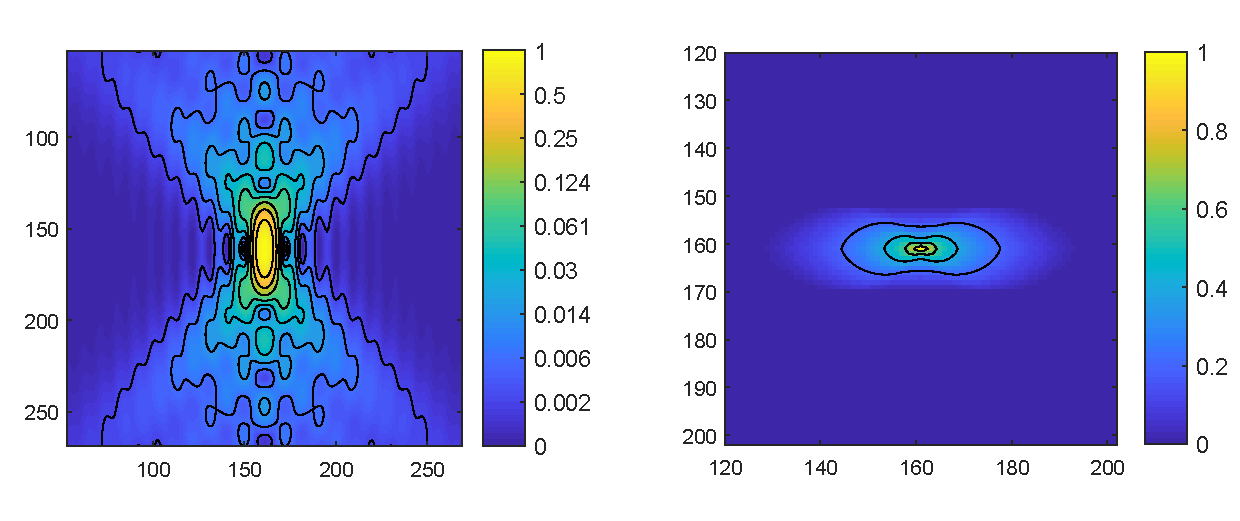
\includegraphics[width=1\textwidth]{psfs/WF.pdf}
      \bcaption[Axial cross section of the PSF and OTF of a wide-field microscope]{Simulated PSF (left) and OTF (right) for a wide-field microscope with a water immersion objective ($n=1.33$). $NA=1.1$, $\lambda = \SI{510}{nm}$}
      \label{fig:psf-wf}
    \end{figure}


    Abbe's formula can be derived from the scalar theory of diffraction using a paraxial approximation (Fraunhofer diffraction, \cite{born_principles_2013}). It describes the intensity of the electric field in the focus of a lens \cite{sheppard_imaging_1987}:

    \begin{equation}
      H(u,v) = C_0 \left| \int_0^1 J_0 (vr)e^{-i\frac{1}{2}\cdot ur^2} rdr \right|^2,
      \label{eq:psf}
    \end{equation}
    where $C_0$ is a normalization constant, and $J_0$ is the zero order Bessel function of the first kind. Furthermore, instead of the commonly used Cartesian coordinates $x$, $y$ and $z$, the following optical coordinates are defined:
    \begin{equation}
      v = \frac{2\pi n  r}{\lambda_0} \sin \alpha, \quad
      u=\frac{8\pi n  z}{\lambda_0} \sin^2 \frac{\alpha}{2}
      \label{eq:substitutions}
    \end{equation}
    where $r = \sqrt{x^2 + y^2}$ is the distance from the optical axis, and $\alpha$ is the light collection angle as shown on \autoref{fig:wide-field}. 

    To determine the lateral resolution of the system, let's substitute $u=0$ as the axial optical coordinate, and evaluate \autoref{eq:psf} which will give the intensity distribution in the focal plane:
    \begin{equation}
      H(0,v) = C_0 \left| \int_0^1 J_0(vr)rdr \right|^2 = \left(2\frac{J_1(v)}{v} \right) ^2,
      \label{eq:airy}
    \end{equation}
    \begin{figure}
      \centering
      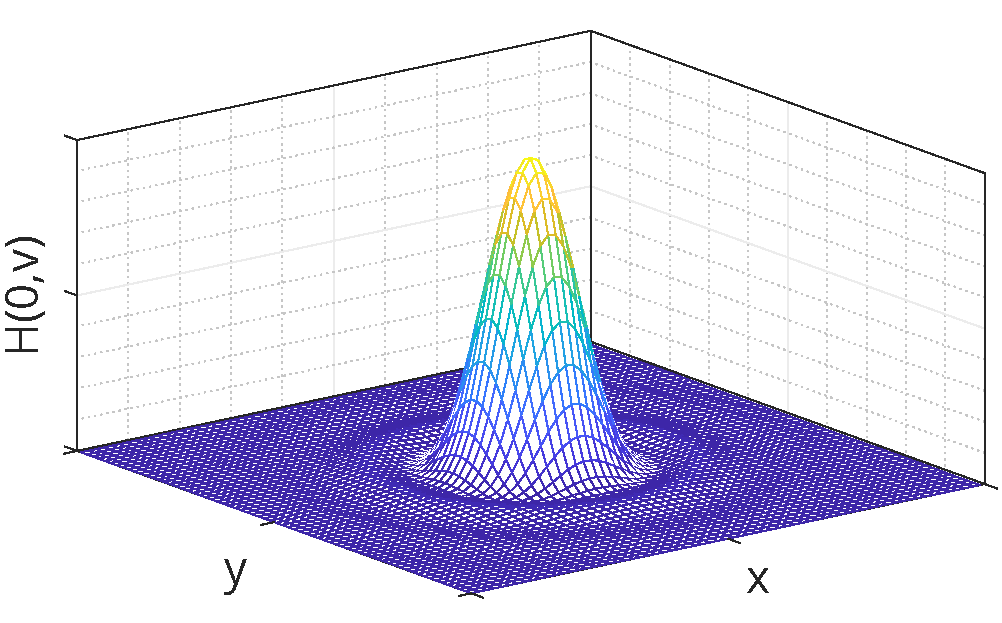
\includegraphics[width=0.7\textwidth]{airy}
      \bcaption[Airy pattern]{Airy pattern calculated in Matlab based on \autoref{eq:airy}}
      \label{fig:airy}
    \end{figure}


    

    where $J_1$ is the first order Bessel function of the first kind.
    % potentially first-order Bessel function
    This equation describes the famous Airy pattern (\autoref{fig:airy}) which will be the shape of the PSF in the focal plane. The width of this pattern is the resolution, and although there are multiple definitions for this, the most commonly accepted is the Rayleigh criterion \cite{f.r.s_xxxi._1879, born_principles_2013} which defines the resolution as the distance between the central peak and the first local minimum. As this lies at $v=3.38$, the resolution can be expressed by substituting this value into \autoref{eq:substitutions} and solving it for $r$:
    \begin{equation}
      \delta_{xy} = r(v=0.338) = \frac{3.83}{2\pi} \frac{\lambda_0}{n\cdot \sin \alpha} \approx 0.61 \frac{\lambda_0}{NA},
      \label{eq:lateralRes}
    \end{equation}
    which is equivalent to Abbe's original formula (\autoref{eq:abbe}). The only difference is the scaling factor which is due to the slightly different interpretations of width of the Airy disk as mentioned earlier.

    Similarly, to calculate the intensity distribution along the axial direction, let's substitute $v=0$ to \autoref{eq:psf}:
    \begin{equation}
      H(u,0)=C_0\left( \frac{\sin \frac{u}{4}}{\frac{u}{4}}\right) ^2 . 
    \end{equation} 
    For this expression the first minimum lies at $u=4\pi$. Converting back to Cartesian coordinates, the axial resolution can be expressed as:
    \begin{equation}
      \delta_z = \frac{2n\lambda_0}{NA^2}.
      \label{eq:axialRes}
    \end{equation}

    So far we only considered a single, point-like emitter. As the intensity function describes how an optical system ``spreads out" the image of a point, it is also called the Point Spread Function (PSF, \autoref{fig:psf-wf}). In a more realistic scenario, however the emitters are neither point-like, nor single. Effectively, however, for every emitter the PSF would be imaged on the sensor, and this creates the final image. In mathematical terms, this can be expressed as a convolution operation between the underlying fluorophore distribution of the object ($O$) and the PSF ($H$):
    \begin{equation}
      I(u,v) = O(u,v) * H(u,v).
    \end{equation}

    The effective result of this kind of diffraction-limited image formation is a blurred image with a finite resolution of $\delta_{xy}$ in the lateral direction, and $\delta_z$ in the axial direction.

    The PSF is further affected by the illumination pattern as well. Since the number of emitted fluorescent photons are roughly proportional to the illumination intensity, the illumination pattern will have an effect on the overall PSF of the system, which can be expressed as:
    \begin{equation}
      H_{sys} = H_{ill} \cdot H_{det},
      \label{eq:systemPSF}
    \end{equation}
    where $H_{ill}$ is the point spread function of the illumination, and $H_{det}$ is the point spread function of the detection.



\section{Point scanning methods}
  In most cases, a wide-field microscope is used to image a layer of cells, of a sectioned sample, thus axial resolution is not a concern. Imaging live specimens, however is not so straightforward, as these samples are usually much thicker than a typical section. For these samples 3-dimensional (3D) imaging is highly beneficial, which necessitates some kind of optical sectioning technique to be able to discriminate the features at different depths.


  Due to the design of the wide-field microscope, any photons emitted from outside the focal plane will also be detected by the sensor, however as these are not originating from the focus, only a blur will be visible. This blur potentially degrades image quality and signal-to-noise ratio to such an extent that makes imaging thick samples very difficult if not impossible in a wide-field microscope. 

  % In the previous section we defined optical resolution, and derived the formulas to calculate the lateral and axial resolutions. These formulas, however are not completely accurate for high NA imaging, since the derivation itself depended on a paraxial approximation of the Kirchhoff diffraction equation. A more robust, and generally accepted method to calculate the resolution for high-NA objectives is the Stelzer-Grill-Heisenberg (SGH) theory
  % \cite{grill_method_1999, stelzer_uncertainty_2000}:
  % \begin{equation} \label{eq:latres}
  % \sigma_{xy}=\frac{\lambda}{\sqrt{3-2 \cos \alpha - \cos 2 \alpha}}
  % \end{equation}
  % \begin{equation} \label{eq:axres}
  % \sigma_z = \frac{\lambda}{1-\cos \alpha}
  % \end{equation}

  \begin{figure}
    \centering
    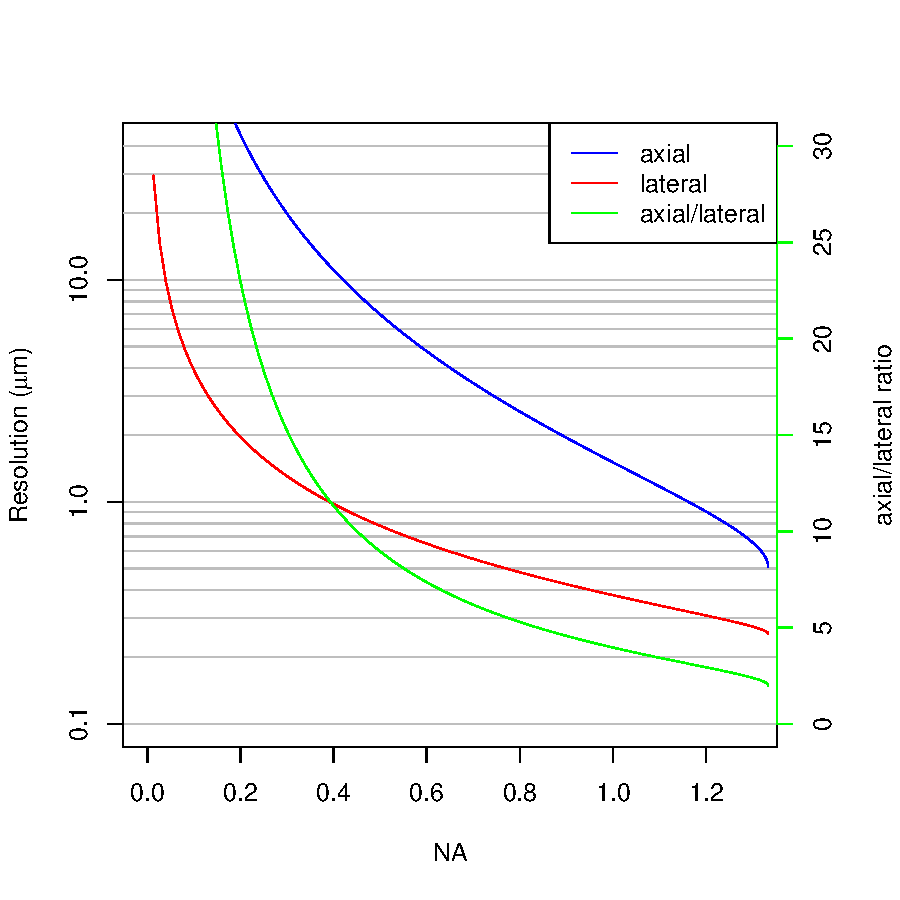
\includegraphics[width=0.55\textwidth]{resolution}
    \bcaption[Resolution of a wide-field microscope]{Axial (blue) and lateral (red) resolutions of a wide-field microscope are shown with respect to the numerical aperture (NA). Resolutions are calculated with $\lambda =510nm$, the emission maximum of GFP and $n=1.33$, the refractive index of water, for water dipping objectives.}
    \label{fig:resolution}
  \end{figure}

  Evaluating Equations \ref{eq:lateralRes} and \ref{eq:axialRes} for a range of possible numerical apertures reveals the significant differences in lateral and axial resolution for any objective (\autoref{fig:resolution}). Especially for low NAs, this can be significant, a factor of $\sim$20 difference. For higher (>0.8) NAs the axial resolution increases faster than the lateral, however they will only be equal when $\alpha=\SI{180}{\degree}$. This means that isotropic resolution with a single lens is only possible if the lens is collecting all light emitting from the sample, which seems hardly possible, and would be highly impractical. For commonly used high NA objectives the lateral to axial ratio will still be around 3--6. 

  Instead of using a single lens to achieve isotropic resolution, it is more practical to image the sample from multiple directions to complement the missing information from different views. When rotating the sample by \SI{90}{\degree} for example, the lateral direction of the second view will correspond to the axial direction of the first view. If rotation is not possible, using multiple objectives can also achieve similar results, such as in the case of Multi-Imaging Axis Microscopy (MIAM) \cite{swoger_multiple_2003,swoger_multi-view_2007}. This microscope consisted of 4 identical objectives arranged in a tetrahedral fashion to collect as much light as possible from multiple directions, and provide isotropic 3D resolution, albeit at the expense of extremely difficult sample handling, since the sample was surrounded by objectives from all directions. 

  % Another disadvantage of the wide-field microscope, is that it can not be used with thick specimens. Usually this type of microscopy is only used for a single layer of cells, because all the objects in the field of view will appear on the imaging plane, not just the plane in focus. These objects will appear blurred if close to the focus, or just evenly add to the background noise if they are further from the focus. This is why imaging specimens much thicker than $10\ \mu m$ will result in suboptimal image quality.





%  ####    ####   #    #  ######   ####    ####     ##    #      
% #    #  #    #  ##   #  #       #    #  #    #   #  #   #      
% #       #    #  # #  #  #####   #    #  #       #    #  #      
% #       #    #  #  # #  #       #    #  #       ######  #      
% #    #  #    #  #   ##  #       #    #  #    #  #    #  #      
%  ####    ####   #    #  #        ####    ####   #    #  ###### 
                                                              

  \subsection{Confocal laser scanning microscopy}

    Confocal laser scanning microscopy (CLSM) \cite{minsky_microscopy_1961,davidovits_scanning_1969} addresses most of the problems of wide-field microscopy we mentioned in the previous section. It is capable of optical sectioning by rejecting out-of-focus light, which makes it a
    true % what?
    3D imaging technique. Furthermore, the light rejection also massively reduces out-of-focus background, and increases contrast.

    This is achieved by two significant modifications compared to the wide-field optical path. To be able to reject the out-of-focus light, an adjustable pinhole is placed at the focus of the tube lens. Light rays originating from the focal point will meet here, and are able to pass through the pinhole. However, out-of-focus light will converge either before or after the aperture, and thus the aperture blocks these rays. To maximize the fluorescence readout efficiency for the single focal point, a photomultiplier tube is used instead of an area sensor (\autoref{fig:confocal}).

    \begin{figure}[tb]
    \begin{subfigure}[t]{0.49\textwidth}
      \centering
      \includegraphics[page=3,width=\textwidth]{spim_cyl}
      \caption{\textbf{Confocal microscope}}
      \label{fig:confocal}
    \end{subfigure}
    \begin{subfigure}[t]{0.49\textwidth}
      \centering
      \includegraphics[page=5,width=\textwidth]{spim_cyl}
      \caption{\textbf{Confocal-theta microscope}}
      \label{fig:conf-theta}
    \end{subfigure}
    \bcaption[Basic optical components of a confocal laser scanning and confocal-theta microscope]{Both types of microscopes use confocal image detection, which means that a pinhole is used to exclude light coming from out-of-focus points. Light intensity is measured by a photomultiplier for every point in the region of interest. The final image is generated on a computer using the positions and recorded intensity values. A regular confocal microscope (a) uses the same objective for illumination and detection, while a confocal-theta microscope (b) uses a second objective that is rotated by $\theta$ around the focus. In this case, $\theta = 90^\circ$.}
    \label{fig:confocals}
    \end{figure}

    To maximize the signal from the focal point, the illumination light is also focused here by coupling an expanded laser beam through the back aperture of the objective. This not only increases illumination efficiency (since other, not detected points are not illuminated), but has the added benefit of increasing the resolution as well. This is due to the combined effect of illumination and detection PSFs as described in \autoref{eq:systemPSF} (\autoref{fig:psf-confocal}). For Gaussian-like PSFs, the final resolution (along a single direction) can be calculated in the following way:
    \begin{equation}
      \frac{1}{\delta _{sys}^2} = \frac{1}{\delta _{ill}^2} + \frac{1}{\delta _{det}^2},
      \label{eq:systemRes}
    \end{equation}
    where $\delta_{ill}$ and $\delta_{det}$ are the resolutions for the illumination and detection, respectively. Since the same objective is used for both illumination and detection, and the difference in wavelength is almost negligible, $\delta_{ill} = \delta_{det} = \delta$, the final system resolution will be:
    \begin{equation}
      \delta_{sys} = \frac{1}{\sqrt{2}} \delta.
    \end{equation}
    This means that the distinguishable features in a confocal microscope are $\sim$0.7 times smaller than in a wide-field microscope using the same objective.

    Because of the different detection method in a confocal microscope, direct image formation on an area sensor is not possible, since at any given time, only a single point is interrogated in the sample. Instead, it is necessary to move the illumination and detection point in synchrony (or in a simpler, albeit slower solution, to move the sample) to scan the entire field of view. The image can be later computationally reconstructed by a computer program that records the fluorescence intensity of every point of the field of view, and displays these values as a raster image.


    \begin{figure}
      \centering
      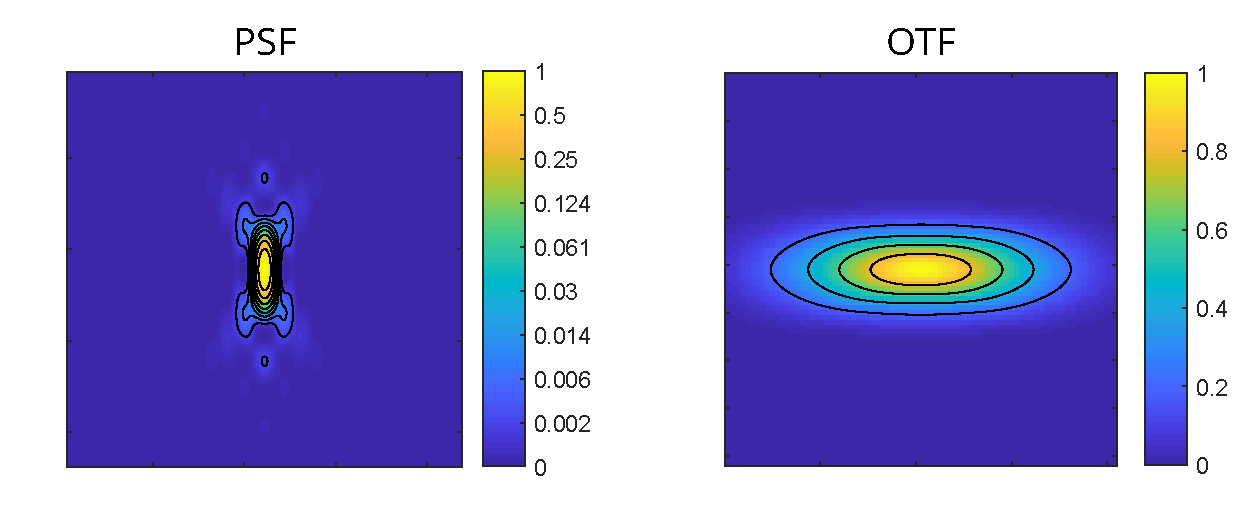
\includegraphics[width=1\textwidth]{psfs/confocal.pdf}
      \bcaption[Axial cross section of the PSF and OTF of a confocal laser scanning microscope]{Simulated PSF and OTF for a laser scanning confocal microscope with a water immersion objective ($n=1.33$). $NA=1.1$, $\lambda = \SI{510}{nm}$}
      \label{fig:psf-confocal}
    \end{figure}


  \subsection{Confocal-theta microscopy}

    % Although confocal microscopy already provides a better resolution in all dimensions, the ratio of the axial and lateral resolution is still very high, due to the single objective illumination and detection. This seriously limits the microscope's 3D imaging capabilities, since in the $z$ direction (i.e. along the imaging axis) the resolution would be significantly worse than in the other directions.
    Although confocal microscopy already has 3D capabilities, its axial resolution is still limited compared to the lateral, since it uses only one objective. An alternative realization of the confocal microscope, the confocal theta microscope \cite{stelzer_fundamental_1994} introduces a second objective to the system, that is used to illuminate the sample (\autoref{fig:conf-theta}). Since this decouples the illumination and detection, using a dichroic mirror is no longer necessary. The second objective is rotated by $\theta$ around the focus, this is where the name of this setup originates from.

    As in the case of standard confocal microscopy, the system PSF is improved by the illumination pattern. Here, however, the axial direction of the detection coincides with the lateral direction of the illumination, which results in a dramatic improvement of axial resolution compared to standard confocal microscopy. Lateral resolution will also be increased, but by a smaller extent, resulting in an almost isotropic PSF, and equal axial and lateral resolutions. % (\autoref{fig:psf-theta}).
    Although this is a big improvement to confocal microscopy in terms of resolution, this technique did not reach a widespread adoption as it complicates sample handling, while still suffering from two drawbacks of confocal microscopy that limit its live imaging capabilities.

    Imaging live specimens for an extended period of time with confocal microscopy although possible \cite{aldaz_live_2010, maitre_asymmetric_2016}, is not ideal. For each voxel imaged, a large portion of the specimen has to be illuminated, which results in a very high dose of radiation on the sample. This can be as much as 30--100 times larger, than the dose used for the actual imaging \cite{reynaud_light_2008}. Illumination with high power of laser for an extended time frame can result in bleaching the fluorophores, which in turn will lower the signal at later times. Furthermore, any absorbed photon has the possibility to disrupt the chemical bonds inside the specimen, which can lead to phototoxic effects. Moreover, the usage of the pinhole although increases resolution, also decreases the detectable signal intensity, thus has a negative impact on image contrast \cite{stelzer_contrast_1998}.

  % \subsection{Mammalian imaging with confocal microscopy}
    


%  ######  ########  #### ##     ## 
% ##    ## ##     ##  ##  ###   ### 
% ##       ##     ##  ##  #### #### 
%  ######  ########   ##  ## ### ## 
%       ## ##         ##  ##     ## 
% ##    ## ##         ##  ##     ## 
%  ######  ##        #### ##     ## 


\section{Light-sheet microscopy}
  \label{sec:light-sheet}
  \begin{figure}[bt]
    \centering
    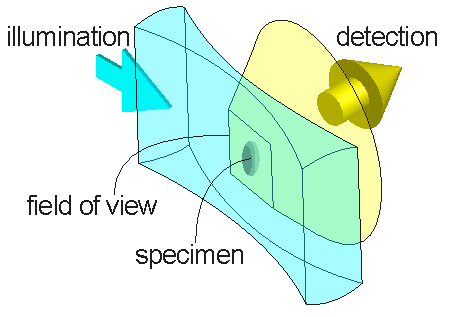
\includegraphics[width=0.6\textwidth]{spim_concept}
    \bcaption[Basic concept of single-plane illumination microscopy]{The sample is illuminated from the side by laser light shaped to a light-sheet (blue). This illuminates the focal plane of the detection lens, that collects light in a wide-field mode (yellow). The image is recorded, and the sample is translated through the light-sheet to acquire an entire 3D stack.}
    \label{fig:spim_concept}
  \end{figure}

  A selective-plane illumination microscope (SPIM) uses a light-sheet to illuminate only a thin section of the sample (\autoref{fig:spim_concept}). This illumination plane is perpendicular to the imaging axis of the detection objective and coincides with the focal plane. This way, only the section in focus will be illuminated, thus providing much better signal to noise ratio. In case of conventional wide-field fluorescence microscopy, where the whole specimen is illuminated, out-of-focus light contributes to a significant background noise. 
  With selective-plane illumination, this problem is intrinsically solved, and it also provides a true optical sectioning capability. This makes SPIM especially suitable for 3D imaging.

  

  The main principle behind single-plane illumination microscopy, that is illuminating the sample from the side by a thin light-sheet, dates back to the early 20\textsuperscript{th} century, when Siedentopf and Zsigmondy first described the ultramicroscope \cite{siedentopf_uber_1902}. This microscope used sunlight as an illumination source, that was guided through a precision slit to generate a thin light-sheet. This allowed Zsigmondy to visualize gold nanoparticles floating in and out of the light-sheet. Since these particles are much smaller than the wavelength of the light, the device was called an ultramicroscope. His studies with colloids, and the development of the ultramicroscope led Zsigmondy to win the Nobel Prize in 1925.

  After Zsigmondy, this method was forgotten until rediscovered in the 1990s, when Voie \etal constructed their Orthogonal-plane Fluorescent Optical Sectioning (OPFOS) microscope \cite{voie_orthogonal-plane_1993}. They used it to image a fixed, optically cleared and fluorescently labelled guinea pig cochlea. In order to acquire a 3D dataset, the sample was illuminated from the side with a light-sheet generated by a cylindrical lens, then rotated around the center axis to obtain multiple views. Although they only reached a lateral resolution around \SI{10}{\micro m} and axial resolution of \SI{26}{\micro m}, this method allowed them to generate a 3D reconstruction of the guinea pig cochlea \cite{voie_three-dimensional_1995}.

  Later, in 2002, Fuchs et al. developed Thin Light-Sheet Microscopy (TLSM) \cite{fuchs_thin_2002} and used this technique to investigate the microbial life in seawater samples without disturbing their natural environment (by e.g. placing them on a coverslip). Their light-sheet was similar to the one utilized in OPFOS, being \SI{23}{\micro m} thin, and providing a $\SI{1}{mm} \times \SI{1}{mm}$ field of view.

  Despite these early efforts, the method did not gain larger momentum. The real breakthrough in light-sheet imaging happened at the European Molecular Biology Laboratory (EMBL) in 2004, where Huisken \etal \cite{huisken_optical_2004} combined the advantages of endogenous fluorescent proteins and the optical sectioning capability of light-sheet illumination to image Medaka fish embryos, and the complete embryonic development of a \textit{Drosopila melanogaster} embryo. They called this Selective-Plane Illumination Microscopy (SPIM), and it quickly became popular to investigate developmental biological questions.

  \label{sec:multiview}
  \begin{figure}[tb]
    \centering
    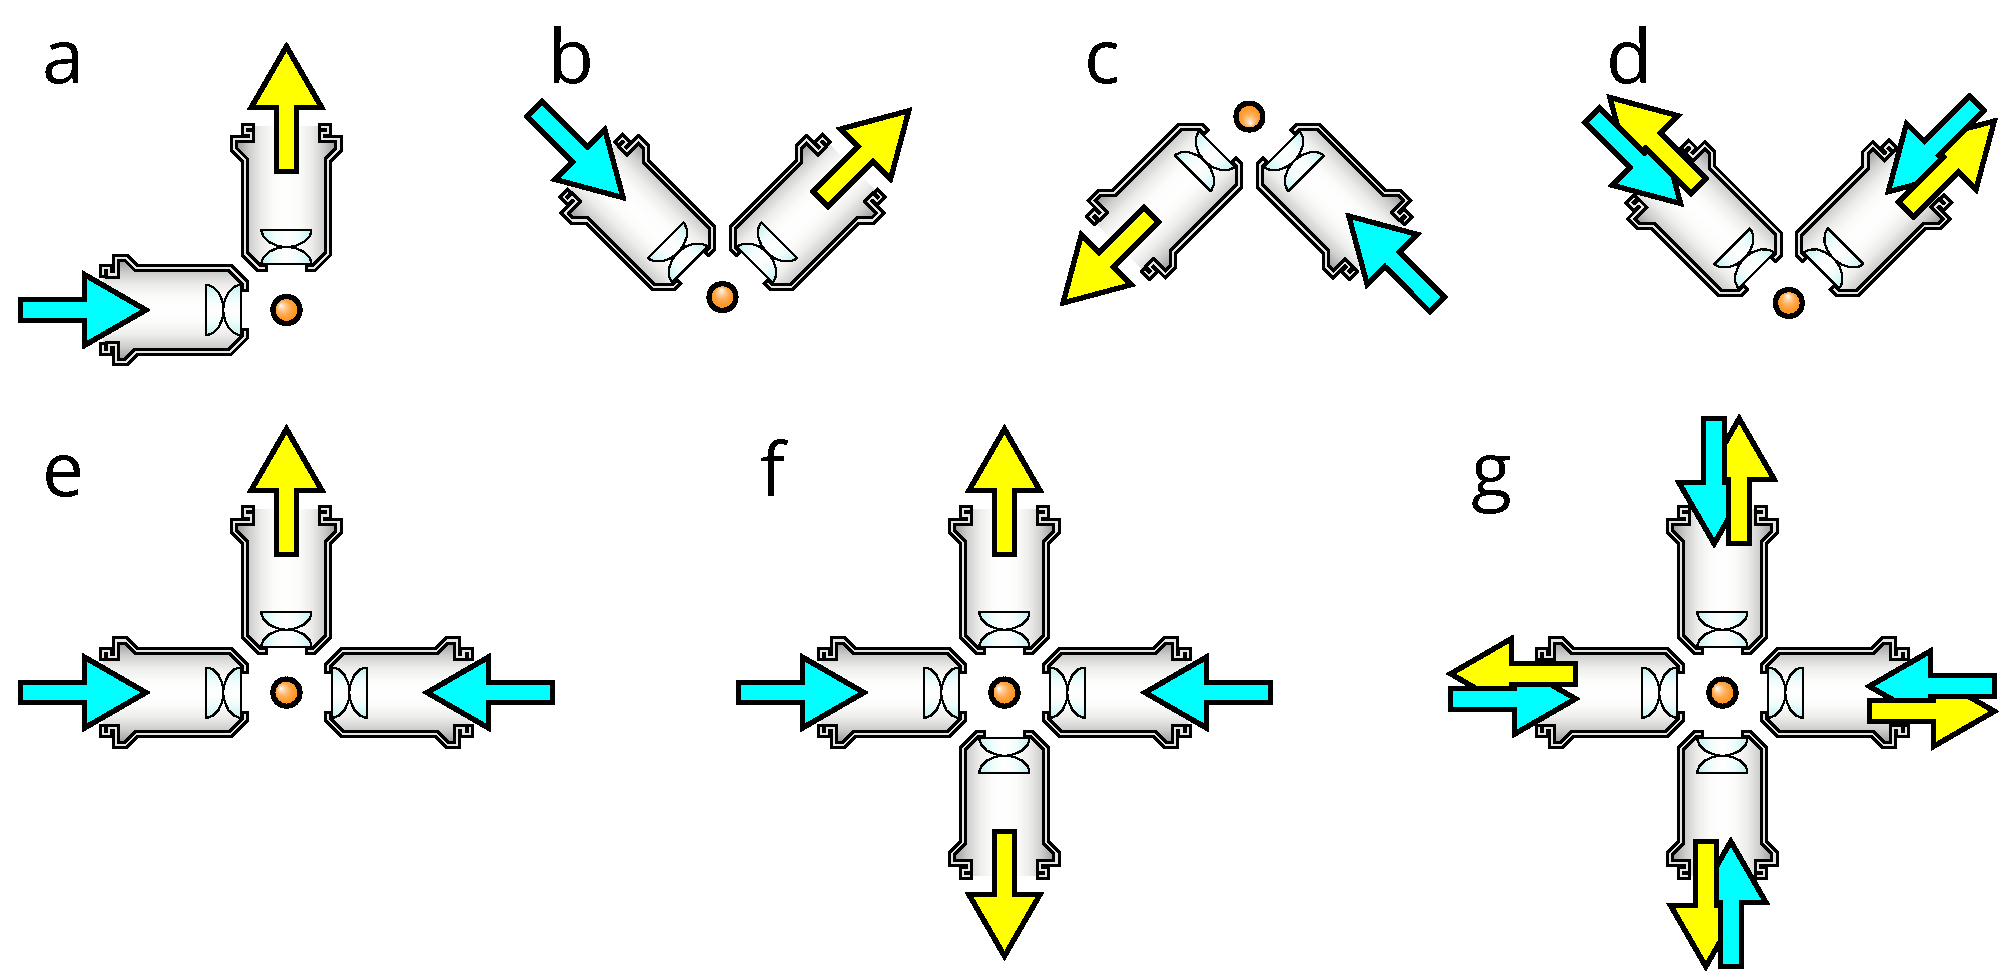
\includegraphics[width=\textwidth]{spim_zoo}
    \bcaption[Different optical arrangements for light-sheet microscopy]{\textbf{(a)} Original SPIM design with a single lens for detection and illumination. \cite{huisken_optical_2004} \textbf{(b)} Upright SPIM to allow for easier sample mounting such as using a petri dish (iSPIM, \cite{capoulade_quantitative_2011, wu_inverted_2011, hoyer_breaking_2016}). \textbf{(c)} Inverted SPIM, where the objectives are below the sample, which is held by a thin foil \cite{strnad_inverted_2016}. \textbf{(d)} Dual-view version of the upright configuration, where both objective can be used for illumination and detection (diSPIM, \cite{wu_spatially_2013}). \textbf{(e)} Multidirectional-SPIM (mSPIM) for even illumination of the sample with two objectives for illumination \cite{huisken_even_2007}. \textbf{(f)} Multi-view SPIM with two illumination and detection objectives for \textit{in toto} imaging of whole embryos (MuVi-SPIM \cite{krzic_multiview_2012}, SimView \cite{tomer_quantitative_2012}, Four-lens SPIM \cite{schmid_high-speed_2013}). \textbf{(g)} A combination of (d) and (f), using four identical objectives, where both can illuminate and detect in a sequential manner, to achieve isotropic resolution without sample rotation (IsoView \cite{chhetri_whole-animal_2015}).}
    \label{fig:spim_zoo}
  \end{figure}
  
  Since then, light-sheet-based imaging has gained more and more popularity, as it can be adapted and applied to a wide variety of problems. Although sample mounting can be challenging because of the objective arrangement, this can also be an advantage, since new microscopes can be designed with the sample in mind \cite{huisken_selective_2009, de_medeiros_light-sheet_2016} (\autoref{fig:spim_zoo}). This made it possible to adapt the technique for numerous other specimens, such as zebrafish larvae \cite{keller_reconstruction_2008}, \textit{C. elegans} embryos \cite{wu_inverted_2011}, mouse brain \cite{dodt_ultramicroscopy:_2007}, and even mouse embryos \cite{ichikawa_live_2013, udan_quantitative_2014, strnad_inverted_2016}.

  As many of these specimens require very different conditions and mounting techniques, these microscopes have been adapted to best accommodate them. An upright objective arrangement for example (\autoref{fig:spim_zoo}b) allows imaging samples on a coverslip, while its inverted version is well suited for mouse embryos, where a foil is separating them from the immersion medium (\autoref{fig:spim_zoo}c). A modified version of the upright arrangement allows for multi-view imaging using both objectives for illumination and detection in a sequential manner (\autoref{fig:spim_zoo}d) \cite{kumar_dual-view_2014}.

  To achieve a more even illumination in larger samples, two objectives can be used from opposing directions to generate two light-sheets (\autoref{fig:spim_zoo}e) \cite{huisken_even_2007}. This arrangement can further be complemented by a second detection objective, to achieve parallelized multi-view imaging (\autoref{fig:spim_zoo}f) \cite{krzic_multiview_2012,tomer_quantitative_2012, schmid_high-speed_2013}. For ultimate speed, 4 identical objectives can be used to achieve almost instantaneous views from 4 different directions by using all objectives for illumination and detection (\autoref{fig:spim_zoo}g) \cite{chhetri_whole-animal_2015}. 

  Furthermore, because of the wide-field detection scheme it is possible to combine SPIM with many superresolution techniques, such as single molecule localization \cite{cella_zanacchi_live-cell_2011}, STED \cite{friedrich_sted-spim:_2011}, RESOLFT \cite{hoyer_breaking_2016}, or structured illumination \cite{keller_fast_2010,chen_lattice_2014,chang_csilsfm_2017}.




  % \subsection{Optics of light-sheet microscopy}

    
    \begin{figure}[htb]
        \centering
        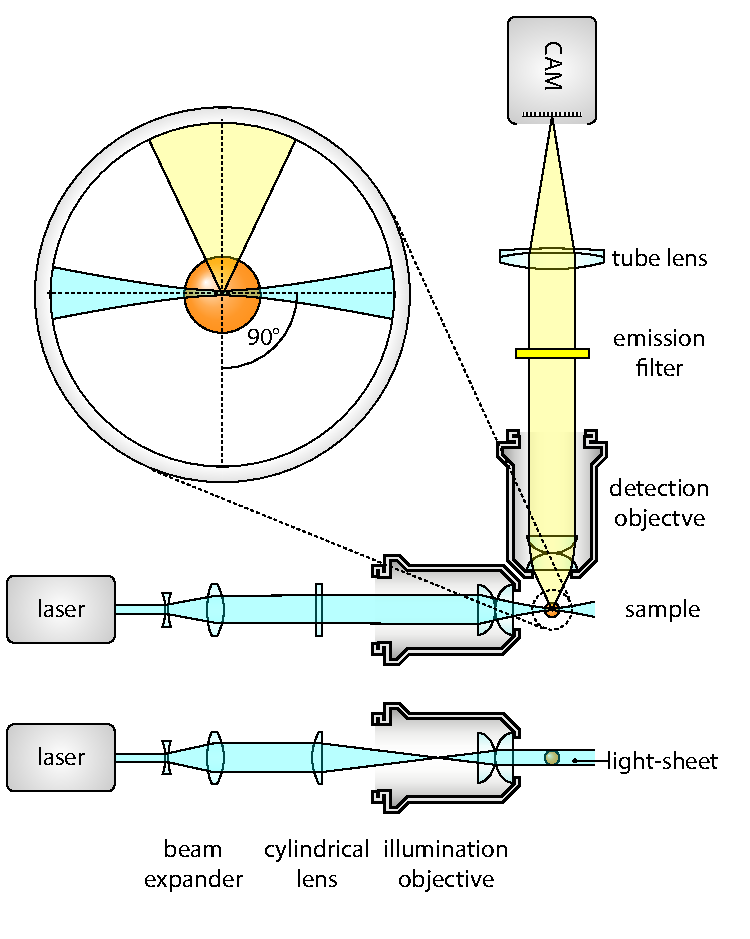
\includegraphics[page=1,width=0.7\textwidth]{spim_cyl}
        \bcaption[Basic optical components of a SPIM]{A dedicated illumination objective is used to generate the light-sheet, which is an astigmatic Gaussian beam, focused along one direction. Astigmatism is introduced by placing a cylindrical lens focusing on the back focal plane of the objective. Detection is performed at a right angle, with a second, detection objective. Scattered laser light is filtered out, and a tube lens forms the image on an area sensor, such as an sCMOS camera.}
        \label{fig:light-sheet}
    \end{figure}

    % \begin{figure}
    %     \centering
    %     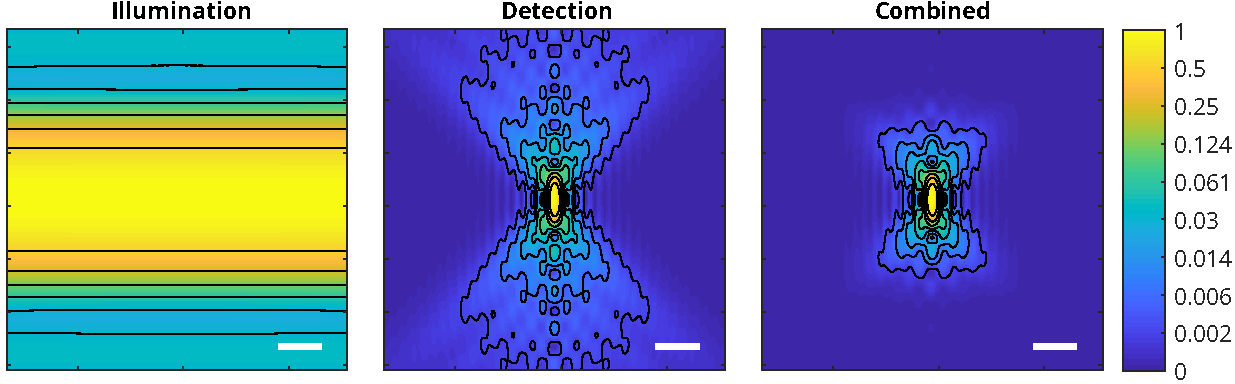
\includegraphics[width=1\textwidth]{psfs/psf_spim.pdf}
    %     \bcaption[Axial cross section of the PSF in a light-sheet microscope]{Simulated PSFs for illumination (left, NA = 0.1, $\lambda = \SI{488}{nm}$) and detection (center, NA=1.1, $\lambda = \SI{510}{nm}$). The system PSF is the multiplication of these PSFs (right).($n=1.33$). Because of the illumination scheme, the light-sheet microscope has a better axial resolution than a conventional wide-field setup.}
    %     \label{fig:psf-spim}
    % \end{figure}


  % \subsection{Detection}
    Since illumination and detection for light-sheet microscopy are decoupled, two independent optical paths are implemented.
    
    The detection unit of a SPIM is basically equivalent to a detection unit of a wide-field microscope, without a dichroic mirror (\autoref{fig:light-sheet}). The most important components are the objective together with the tube lens, filter wheel, and a sensor, typically a CCD or sCMOS camera.

    One of the most important aspects that determines the resolution of the microscope is the detection objective. Since imaging biological specimens usually requires a water-based solution, the objectives also need to be directly submerged in the medium to minimize spherical aberrations. Since the refraction index of water ($n=1.33$) is greater than the refraction index of air, these objectives tend to have a higher NA, resulting in higher resolution. As the illumination is decoupled in this system, the light-sheet thickness also has an influence on the axial resolution. Finally, the resolution also depends on the pixel size of the sensor which determines the spatial sampling rate of the image.

    Although image quality and resolution greatly depend on the detection optics, the real strength of light-sheet microscopy is the inherent optical sectioning which is due to the specially aligned illumination pattern, that confines light to the vicinity of the detection focal plane.

    There are two most commonly used options to generate a light-sheet: either by using a cylindrical lens, to illuminate the whole field of view with a static light-sheet, as in the original SPIM concept \cite{huisken_optical_2004}; or by quickly scanning a thin laser beam through the focal plane, thus resulting in a virtual light-sheet. This method is called Digitally Scanned Light-sheet Microscopy (DSLM) \cite{keller_reconstruction_2008}.


  % \subsection{Illumination}

  \subsection{Static light-sheet illumination}
    For a static light-sheet, the normally circular Gaussian laser beam needs to be shaped in an astigmatic manner, i.e. either expanded or squeezed along one direction, to shape it into a sheet instead of a beam. This effect can be achieved by using a cylindrical lens, which as the name suggests has a curvature in one direction, but is flat in the other, thus focusing a circular beam to a sheet (\autoref{fig:light-sheet}).
    
    However, to achieve light-sheets that are sufficiently thin for optical sectioning, one would need to use cylindrical lens with a very short focal length, and these are hardly accessible in well corrected formats. For this reason, it is more common to use a longer focal length cylindrical lens in conjunction with a microscope objective, which is well corrected for chromatic and spherical aberrations \cite{greger_basic_2007}. This way, the light-sheet length, thickness and width can be adjusted for the specific imaging tasks.


    \subsubsection{Light-sheet dimensions}
    \label{sec:dimensions}
    \begin{figure}
      \centering
      \begin{subfigure}[b]{0.29\textwidth}
          \centering
          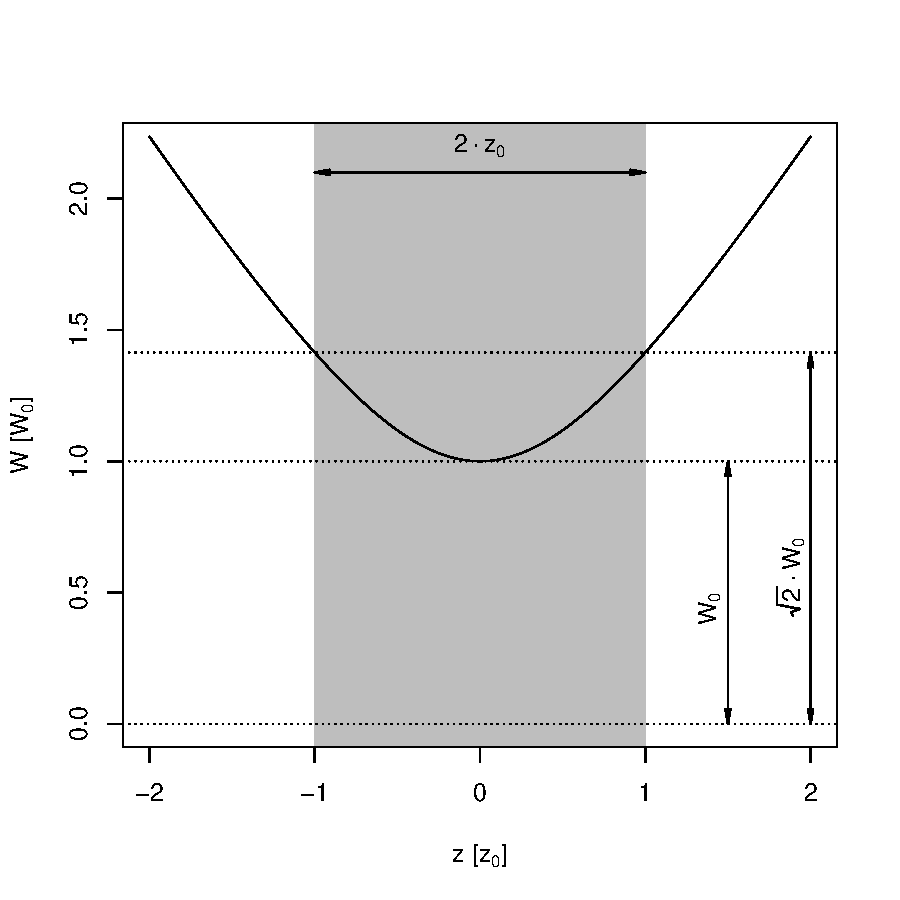
\includegraphics[width=\textwidth]{width}
          \caption{}
          \label{fig:width}
      \end{subfigure}
      \begin{subfigure}[b]{0.29\textwidth}
          \centering
          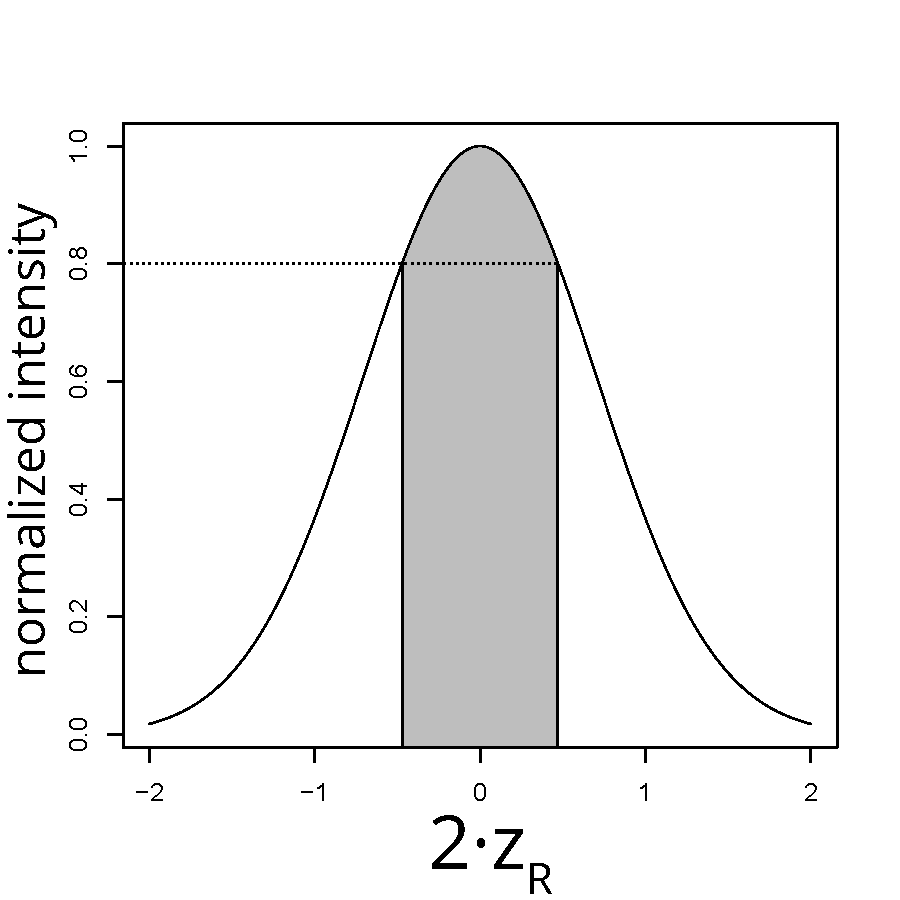
\includegraphics[width=\textwidth]{height}
          \caption{}
          \label{fig:height}
      \end{subfigure}
      \begin{subfigure}[b]{0.39\textwidth}
          \centering
          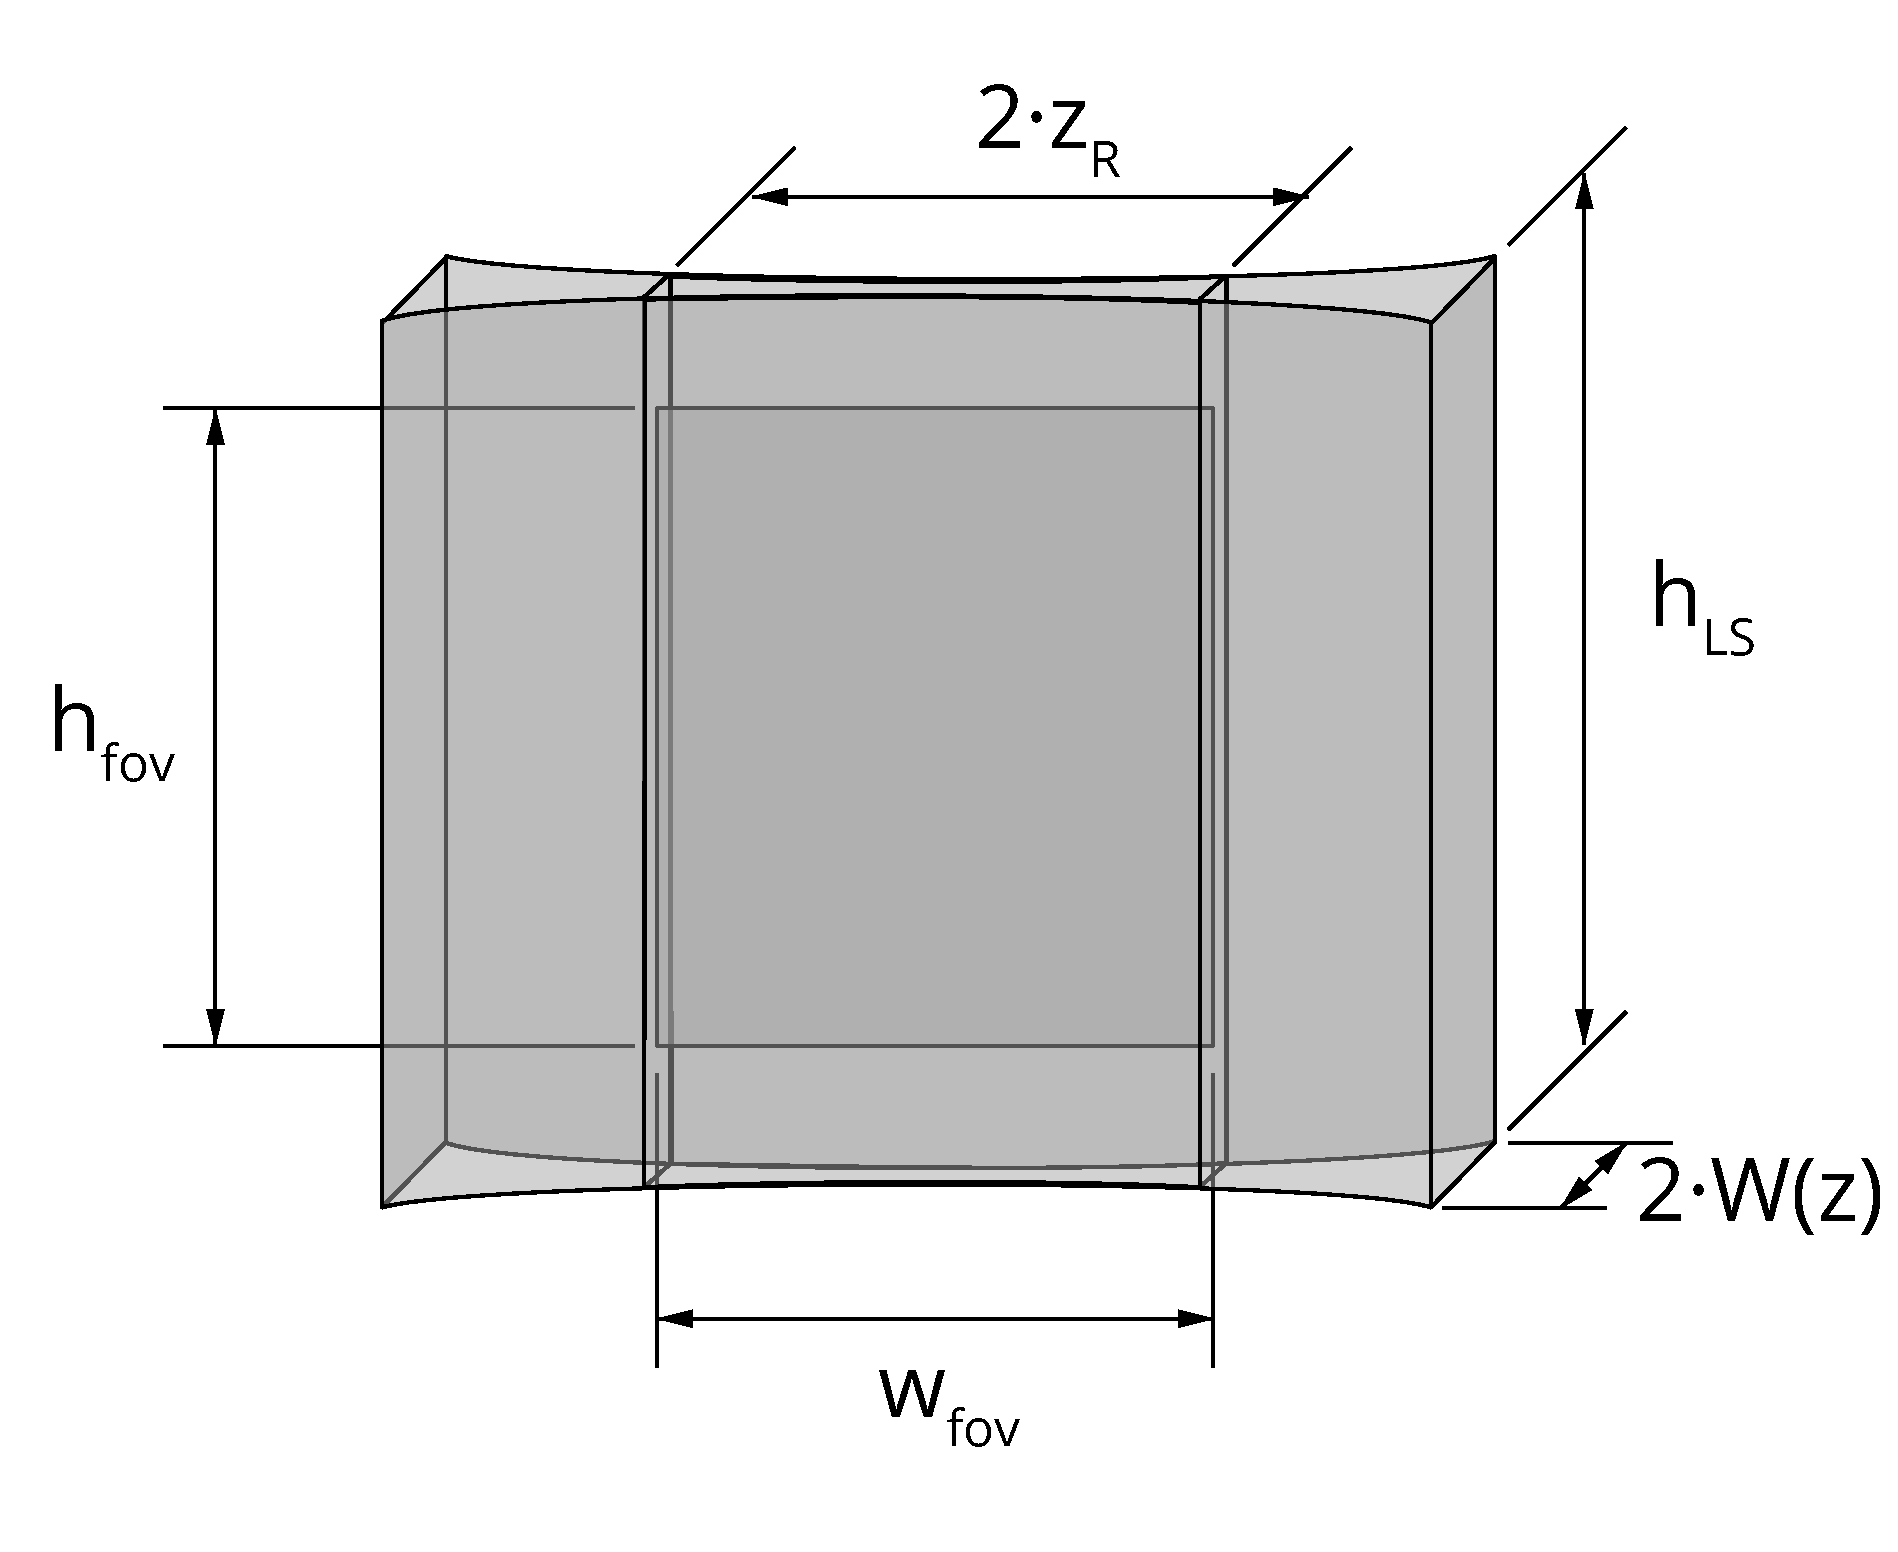
\includegraphics[width=\textwidth]{FOV}
          \caption{}
          \label{fig:fov}
      \end{subfigure}
      \bcaption[Light-sheet dimensions]{(a) The width and thickness of the field of view depends on the Rayleigh length of the beam ($z_{R,y}$) and the beam waist ($W_0$). (b) The height of the field of view is determined by the Gaussian profile of the astigmatic beam. (c) shows a light sheet, with the field of view indicated. Since the light-sheet intensity is uneven, the field of view has to be confined to a smaller region. }
      \label{fig:ls_dim}
    \end{figure}

    The shape of the illumination light determines the optical sectioning capability and the field of view of the microscope, so it is important to be able to quantify these measures. The most commonly used illumination source is a laser beam coupled to a single mode fiber, thus its properties can be described by Gaussian beam optics.

    For paraxial waves, i.e. waves with nearly parallel wave front normals, a general wave equation can be approximated with the paraxial Helmholtz equation \cite{saleh_fundamentals_2007}
    \begin{equation}
      \nabla_T^2 U + i 2k \frac{\partial U}{\partial z} = 0
      \label{eq:helmholtz}
    \end{equation}
    where $\nabla_T^2 = \frac{\partial^2}{\partial x^2} + \frac{\partial^2}{\partial y^2}$, $U(\vec{r})$ is the wave function, $k=\frac{2\pi}{\lambda}$ is the wavenumber and $z$ is in the direction of the light propagation.
    
    A simple solution to this differential equation is the Gaussian beam:
    \begin{equation}
      U(r,z) = A_0 \cdot \frac{W_0}{W(z)} \cdot e^{-\frac{r^2}{W^2(z)}}\cdot e^{-i\cdot \phi(r,z)}
    \label{eq:gaussian}
    \end{equation}
    where $A_0$ is the amplitude of the wave, $W_0$ is the radius of the beam waist (the thinnest location on the beam), $r=\sqrt{x^2+y^2}$ is the distance from the center of the beam, $W(z)$ is the radius of the beam  at distance $z$ from the waist, and $\phi(r,z)$ is the combined phase part of the wave-function (\autoref{fig:width}). Furthermore:

    \begin{equation}
      W(z) = W_0\sqrt{1+\left( \frac{z}{z_\mathrm{R}} \right)^2}
    \end{equation}
    where the parameter $z_\mathrm{R}$ is called the Rayleigh-range, and is defined the following way:

    \begin{equation}
      z_\mathrm{R} = \frac{\pi W_0^2}{\lambda}.
      \label{eq:rayleigh}
    \end{equation}
    

    % The available height of the field of view depends on the uniformity of the illumination. The intensity of the emitted fluorescence is based on the intensity of the excitation light. In case of a Gaussian beam:
    % \begin{equation}
    %   I(r,z) = U(r,z)\cdot U^*(r,z) = |A_0|^2 \cdot \left( \frac{W_0}{W(z)}\right)^2 \cdot e^{-\frac{2r^2}{W^2(z)}},
    % \end{equation}

    Apart from the circular Gaussian beam, the elliptical Gaussian beam is also an eigenfunction of Helmholtz equation (\autoref{eq:helmholtz}) which describes the beam shape after a cylindrical lens:
    \begin{equation}
      U(x,y,z) = A_0 \cdot \sqrt{\frac{W_{0,x}}{W_x(z-z_{0,x})}} \sqrt{\frac{W_{0,y}}{W_y(z-z_{0,y})}} \cdot e^{-\frac{x^2}{W_x^2(z-z_{0,x})}} \cdot e^{-\frac{y^2}{W_y^2(z-z_{0,y})}} \cdot e^{-i\cdot \phi(x,y,z)}
    \end{equation}
    This beam still has a Gaussian profile along the $x$ and $y$ axes, but the radii ($W_{0,x}$ and $W_{0,y}$), and the beam waist positions ($z_{0,x}$ and $z_{0,y}$) are uncoupled, which results in an elliptical and astigmatic beam. The beam width can now be described by two independent equations for the two orthogonal directions:
    \begin{align}
      W_x(z) = W_{0,x}\sqrt{1+\left( \frac{z}{z_{\mathrm{R},x}} \right)^2}\mathrm{\quad and \quad } W_y(z) = W_{0,y}\sqrt{1+\left( \frac{z}{z_{\mathrm{R},y}} \right)^2}.
    \end{align}
    Since the beam waist is different along the two axes, the Rayleigh range is also different:
    \begin{align}
      z_{\mathrm{R},x} = \frac{\pi W_{x,0}^2}{\lambda}, \quad
      z_{\mathrm{R},y} = \frac{\pi W_{y,0}^2}{\lambda}.
      \label{eq:rayleighXY}
    \end{align}
    % Intensity of the beam is the following:
    % \begin{equation}
    %   I(x,y,z) = U(x,y,z)\cdot U^*(x,y,z) = |A_0|^2 \cdot \frac{W_{x,0}}{W_x(z)} \cdot \frac{W_{y,0}}{W_y(z)} \cdot e^{-\frac{2x^2}{W_x^2(z)}} \cdot e^{-\frac{2y^2}{W_y^2(z)}}
    % \end{equation}
    
    
    Based on these equations, the light-sheet dimensions and usable field of view can be specified (\autoref{fig:fov}). The light-sheet thickness will depend on the beam waist, $W_{0,y}$ (if we assume the cylindrical lens is focusing along $y$), and the length of the light-sheet can be defined as twice the Rayleigh range, $2 \cdot z_{\mathrm{R},y}$. As these are coupled (see \autoref{eq:rayleighXY}), having a thin light-sheet for better sectioning also means that its length will be relatively short. Fortunately, because of the quadratic relation, to increase the field of view by a factor of two, the light-sheet thickness only needs to increase by a factor of $\sqrt{2}$.

    % Since the illumination is uneven, the usable height of the field of view is smaller than the actual illuminated region (\autoref{fig:fov}). The width of the field of view $w_{fov}$ is determined by the Rayleigh length, since this is in a direct relation with the beam divergence. To stay in the optimal region, the light-sheet should only be used in the range of 1 Rayleigh length on both sides of the beam waist (\autoref{fig:width}). In this range, the ratio between the thickest (at $z=z_0$) and the thinnest (at $z=0$) part of the beam $W(z)$ will be $\sqrt{2}\approx 1.4142$ which is still acceptable.

    Light-sheet height is determined by the intensity profile of the beam along the vertical axis (\autoref{fig:height}). Since this is a Gaussian function (see \autoref{eq:gaussian}), only a small part in the middle can be used for imaging, because towards the sides the intensity dramatically drops. To allow a maximum 20\% drop-off in intensity at the edges, the light-sheet height becomes $h_{fov}=2\cdot 0.472\cdot W_{x,0} = 0.944 \cdot W_{x,0}$.
    

  \subsection{Digitally scanned light-sheet illumination}

    \begin{figure}[bt!]
      \centering
      \includegraphics[page=2,width=0.7\textwidth]{spim_cyl}
      \bcaption[DSLM illumination]{DSLM illuminates a specimen by a circularly-symmetric beam that is scanned over the field of view. This creates a virtual light-sheet, which illuminates a section of a specimen just like the SPIM. The light-sheet in DSLM is uniform over the whole field of view and its height can be dynamically altered by changing the beam scan range.
    }
        \label{fig:dslm}
    \end{figure}

    Although generating a static light-sheet is relatively straightforward, with the simple addition of a cylindrical lens to the light path, it has some drawbacks. As already mentioned in the previous section, the light intensity distribution along the field of view is not constant, as the light-sheet is shaped from a Gaussian beam. Furthermore, along the lateral direction of the light-sheet the illumination NA is extremely low, resulting in effectively collimated light. Because of this, shadowing artifacts can deteriorate the image quality \cite{huisken_even_2007}.

    A more flexible way of creating a light-sheet is by scanning a focused beam in the focal plane to generate a virtual light-sheet (digital scanned light-sheet microscopy, DSLM \cite{keller_reconstruction_2008}). Although this method might require higher peak intensities, it solves both drawbacks of the cylindrical lens illumination. By scanning the beam, the light-sheet height can be freely chosen, and a homogenous illumination will be provided. Focusing the beam in all directions evenly introduces more angles in the lateral direction as well, which shortens the length of the shadows.
    
    The basic optical layout of a DSLM is shown on \autoref{fig:dslm}. A galvanometer controlled mirror is used to alter the beam path that can quickly turn around its axis which will result in an angular sweep of the laser beam. To change the angular movement to translation, a scan lens is used to generate an intermediate scanning plane. This plane is then imaged to the specimen by the tube lens and the illumination objective, resulting in a scanned focused beam at the detection focal plane. The detection unit is identical to the wide-field detection scheme, similarly to the static light-sheet illumination. By scanning the beam at a high frequency, a virtual light-sheet is generated, and the fluorescence signal is captured by a single exposure on the camera, resulting in an evenly illuminated field of view.

  



  



% ##     ##  #######  ##     ##  ######  ######## 
% ###   ### ##     ## ##     ## ##    ## ##       
% #### #### ##     ## ##     ## ##       ##       
% ## ### ## ##     ## ##     ##  ######  ######   
% ##     ## ##     ## ##     ##       ## ##       
% ##     ## ##     ## ##     ## ##    ## ##       
% ##     ##  #######   #######   ######  ######## 
\section{Light-sheet microscopy for mouse imaging}

  Because of its optical sectioning capabilities, combined with the high specificity of fluorescent labels, confocal microscopy had an immense influence on biological research, and has been the go-to technique for decades for many discoveries \cite{shotton_confocal_1989,graf_live_2005,jonkman_any_2015}.
  % Even though it has some drawbacks, important discoveries have been made using this technique, as live imaging is not always necessary.
  % Especially using cell cultures, or fixed specimens, confocal microscopy has been used to investigate X chromosome inactivation \cite{costanzi_histone_1998}, the role of amyloid $\upbeta$-peptide in Alzheimer's disease \cite{bard_peripherally_2000}, the role of Oct4 \cite{nichols_formation_1998} and Sox2 \cite{avilion_multipotent_2003} in the self-renewal of pluripotent stem cells, just to highlight a few.
  Live imaging capabilities of confocal microscopy are, however, limited. This is mostly due to the illumination scheme: to collect information from a single point, almost the whole embryo has to be illuminated. This unwanted illumination can easily lead to bleaching of the fluorophores, and also to phototoxic effects that can prevent further embryonic development. The point scanning nature of image acquisition also implies an inherent constraint to the maximum imaging speed, as it can be only increased at the expense of reducing signal intensity (\autoref{fig:tradeoffs}).

  One improvement to address both of these drawbacks is the use of a spinning disk with a specific pattern (also called Nipkow disk) of holes to generate multiple confocal spots at the same time \cite{graf_live_2005}. If these spots are far enough from each other, confocal rejection of out-of-focus light can still occur. As the disk is spinning, the hole pattern will sweep the entire field of view, eventually covering all points \cite{kino_intermediate_1990}. The image is recorded by an area detector, such as a CCD or EM-CCD, which speeds up image acquisition \cite{nakano_spinning-disk_2002}.

  Although out-of-focus illumination is still an issue, spinning disk confocal microscopy was successfully used to investigate the mechanisms of symmetry breaking in early mouse embryonic development \cite{korotkevich_apical_2017}, and the mechanisms leading to the first cell fate specification that will differentiate extraembryonic tissue from the embryo proper \cite{maitre_pulsatile_2015,dietrich_venus_2015,maitre_asymmetric_2016}. Even though these studies were carried out with live embryos, only a few hours of time-lapse imaging is possible before the accumulation of phototoxic effects arrests development \cite{nowotschin_chapter_2010}. Compared to this, just the pre-implantation phase of mouse embryonic development spans 3 days, and the full development is 18 days \cite{wolpert_principles_2011}.


  \subsection{Imaging pre-implantation development}
  \label{ch:mouse-intro}
    Pre-implantation is the first phase of mouse embryonic development, that starts right after fertilization. The embryo in this phase is still in the oviduct, travelling towards the uterus, where it will implant into the uterine wall. The developmental stage between fertilization and the implantation is called the pre-implantation stage. Here the embryo divides, and already the first cell fate specifications start when forming the trophoectoderm (TE) and the inner cell mass (ICM) at the blastocyst stage. ICM cells will form the embryo proper, while TE cell will contribute to the formation of the extraembryonic tissues.
    
    During this process the embryo is still self-sufficient, which makes it possible to image this stage in an \textit{ex vivo} embryo culture by providing the proper conditions \cite{doherty_culture_2000}. Long term imaging, however, is extremely challenging due to the very high light sensitivity of the specimens. Imaging these embryos in a confocal microscope will lead to incomplete development, even if the imaging frequency is minimized to every \SI{15}{mins} \cite{strnad_inverted_2016}.

    Imaging for just a few hours is already enough to investigate important processes, such as cell fate patterning \cite{dietrich_stochastic_2007}. Other approaches aim to lower the phototoxicity by either using 2-photon illumination which operates at longer wavelengths \cite{denk_two-photon_1990,squirrell_long-term_1999,mcdole_lineage_2011}, or by lowering imaging frequency as a compromise \cite{yamagata_long-term_2009}. These approaches, however either require highly specialized equipment, such as an ultra-short pulsed laser, or is compromising on the time resolution.

    Light-sheet microscopy, on the other hand, drastically lowers phototoxic effect by using a much more efficient illumination scheme (see \autoref{sec:light-sheet}), and thus makes a better use of the photon budget. Using this technique, it is possible to image the full pre-implantation development at high spatial and temporal resolution without any negative impact on the developmental process. Such a microscope was developed by Strnad \textit{et al.} at EMBL \cite{strnad_inverted_2016}, who used it to understand when exactly the first cell fate specification is decided in the embryonic cells.

    \begin{figure}[tb]
      \centering
      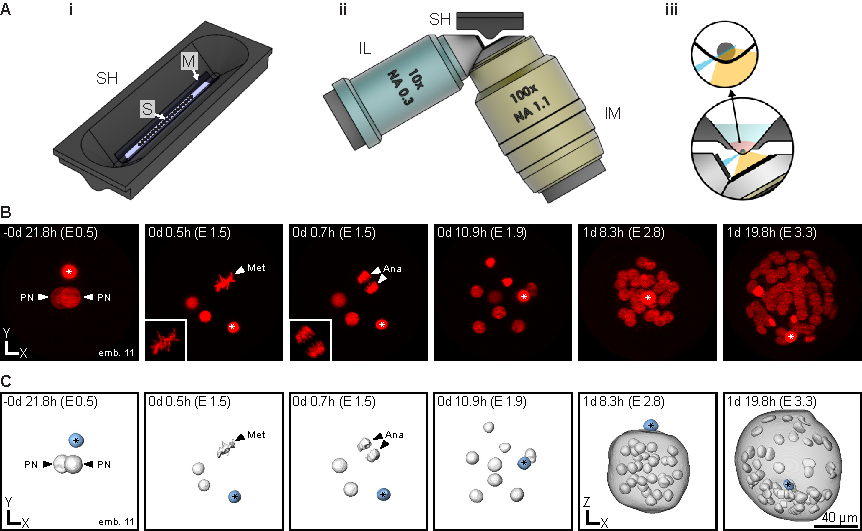
\includegraphics[width=0.8\textwidth]{mammals/Figure2}
      \bcaption[Inverted light-sheet microscope for multiple early mouse embryo imaging.]{(i) A sample holder (SH), containing a transparent FEP membrane (M) allows multiple embryo samples (S) to be placed in line for multisample imaging. (ii) Inverted objective orientation with side view of the sample holder. One possible configuration is to use a 10× 0.3 NA illumination objective (IL) and another 100× 1.1 NA detection objective placed at a right angle to the illumination. (iii) Close up on side view of sample on FEP membrane with both objectives. Since the FEP membrane is transparent on water, it provides no hindrance to the illumination beam in penetrating the sample or for the emitted fluorescence on reaching the detection objective. (B) Still images of one particular timelapse experiment, and (C) corresponding segmented nuclei. The star depicts the polar body. Adapted from Strnad \etal \cite{strnad_inverted_2016}}
      \label{fig:preMouse}
    \end{figure}

    
    As a mouse embryo culture is not compatible with the standard agarose-based sample mounting techniques, a completely new approach was taken, which resulted in a microscope designed around the sample. The sample holder forming a V-shape was built with a bottom window, and it is lined with a thin FEP (fluorinated ethylene propylene) foil that supports the embryos (\autoref{fig:preMouse}A, i). This arrangement allows the utilization of the standard microdrop embryo culture, while providing proper viewing access for the objectives. As the embryos are relatively small (\SI{100}{\micro m}) and transparent, a single illumination and single detection objective arrangement is enough for high quality imaging. A low resolution (NA=0.3) objective is used to generate the scanned light-sheet, and a high resolution (NA=1.1) objective is detecting the fluorescence at 50\texttimes magnification (\autoref{fig:preMouse}A, ii). As the foil is curved, it allows unrestricted access to the embryo, while separating the imaging medium from the immersion liquid (\autoref{fig:preMouse}A, iii). Furthermore, its refractive index is matching the refractive index of water, so optical aberrations are minimized.

    Using this setup, Strnad \textit{et al.} were able to pinpoint the exact timing of the first cell fate decision that leads either to ICM or TE cells. More than 100 embryos expressing nuclear (H2B-mCherry) and membrane (mG) markers were imaged for the entire 3 days of pre-implantation development (\autoref{fig:preMouse}B). The image quality was sufficient to segment all nuclei in the embryos (\autoref{fig:preMouse}C), and track them from 1 to 64 cell stage, building the complete lineage tree. Based on the lineage trees, and the final cell fate assignments, it was determined that at the 16 cell stage the final specification is already decided, while earlier than this it is still random.
    

  \subsection{Imaging post-implantation development}
  
    \begin{figure}[tb]
      \centering
      \includegraphics[width=0.8\textwidth]{mammals/Figure3}
      \bcaption[Imaging mouse post-implantation development]{(A) (i, ii) Mounting technique for E5.5 to E6.5 embryos. A tip-truncated \SI{1}{mL} syringe holds an acrylic rod, cut and drilled with holes of different size in order to best fit the mouse embryo by its Reichert's membrane, leaving the embryo free inside the medium. (iii) Maximum intensity projection of a \SI{13}{\micro m} thick slice at \SI{78}{\micro m} from distal end of an E6.5 mouse embryo. The different tissues corresponding to the rudimentary body plan are annotated. Scale bar: \SI{20}{\micro m}. (B) For stages ranging between E6.5 and E8.5, mounting using a hollow agarose cylinder has also successfully been proposed. Optimal sizes for the corresponding embryonic stage to be imaged can be produced, so that the embryo can grow with least hindrance. (C–F) Steps for mounting the mouse embryo inside the agarose cylinder. The inner volume of the cylinder can be filled with optimal medium, allowing the much larger chamber volume to have less expensive medium. (G–H) Example images of a \SI{9.8}{h} timelapse with the mounting shown in (B) where the expansion of the yolk sac can be observed in direction of the blue arrows. (I) In order to aid multiview light-sheet setups in overcoming the higher scattering properties of embryos at this stage, and to allow faster and easier data recording, electronic confocal slit detection allows better quality images to be taken at shorter acquisition times. Scale bar: \SI{20}{\micro m}. Adapted from Ichikawa \textit{et al.} \cite{ichikawa_live_2013}, Udan \textit{et al.} \cite{udan_quantitative_2014} and de Medeiros and Norlin \textit{et al.} \cite{de_medeiros_confocal_2015}.}
      \label{fig:postMouse}
    \end{figure}

    After the initial 3 days of pre-implantation, the embryo undergoes the implantation process, during which it is inaccessible to microscopical investigations. Although a new method was recently developed that allows the \textit{in vitro} culturing of the embryos embedded in a 3D gel \cite{panavaite_3d-geec:_2017}, this has not reached wider adoption yet. Hence, developmental processes during implantation have only been investigated in fixed embryos.
    
    Following the implantation process, at the post-implantation phase, \textit{ex vivo} embryo culturing becomes possible again \cite{hsu_vitro_1979, huang_effect_2001}, and these embryos can be kept alive for several days in an artificial environment. During this process especially interesting stages are the late blastocyst ($\sim$E4.5), gastrulation ($\sim$E6.5), and somite formation ($\sim$E8.5). Before live imaging techniques became available, these stages were mostly investigated using \textit{in situ} visualization techniques to shed light on several developmental processes \cite{nowotschin_cellular_2010}. Many pathways playing important roles have been identified this way, however live imaging is still necessary to validate these results, and ensure continuity in the same specimen \cite{garcia_live_2011}.

    Light-sheet microscopy is a good choice for imaging these stages, just like in the case of pre-implantation embryos. These embryos, however, present new challenges for sample handling and culturing. Owing to their extreme sensitivity, dissection can be difficult, especially for earlier stages (E4.5). Furthermore, since the embryo is also growing during development, gel embedding is not an option, as this might constrain proper development. Thus, special handling and mounting techniques had to be developed in order to allow live 3D imaging of these specimens.

    Ichikawa \textit{et al.} \cite{ichikawa_live_2013} designed a custom mounting apparatus manufactured from acrylic in the shape of a rod that fits in a standard \SI{1}{mL} syringe with its tip truncated (\autoref{fig:postMouse}A, i). In the rod several holes were drilled with different sizes that can accommodate different sized embryos, which are held by an extraembryonic tissue, the Reichert's membrane (\autoref{fig:postMouse}A, ii). Mounting this way doesn't disturb the embryo itself, and it can freely develop in the culturing medium, while it is also stationary for the purpose of imaging. Using this technique, Ichikawa \textit{et al.} were able to image through several stages of development, including interkinetic nuclear migration at stages E5.5--6.5 (\autoref{fig:postMouse}A, iii).

    A second method of sample mounting for light-sheet imaging was developed by Udan~\etal who were able to record a full \SI{24}{h} time-lapse of living embryos focusing on the gastrulation and yolk sac formation processes (\autoref{fig:postMouse}G--I). Their mounting technique comprised of producing a hollow agarose container shaped like a cylinder that could support the embryo from below without constraining its growth (\autoref{fig:postMouse}B--F).

    Another consideration to keep in mind, is the growing size of the embryo. As it gets bigger, illumination is less efficient, and scattering can dominate at larger depths. As mentioned in earlier (\autoref{sec:multiview}) this can be alleviated by multi-view imaging: illuminating and detecting from multiple directions. Electronic confocal slit detection can further improve the signal to noise ratio by rejecting unwanted scattered light, which allows deeper imaging in large specimens, even up to E7.5 (\autoref{fig:postMouse}I) \cite{de_medeiros_confocal_2015}.

  \subsection{Imaging adult mice}
    
    \begin{figure}
      \centering
      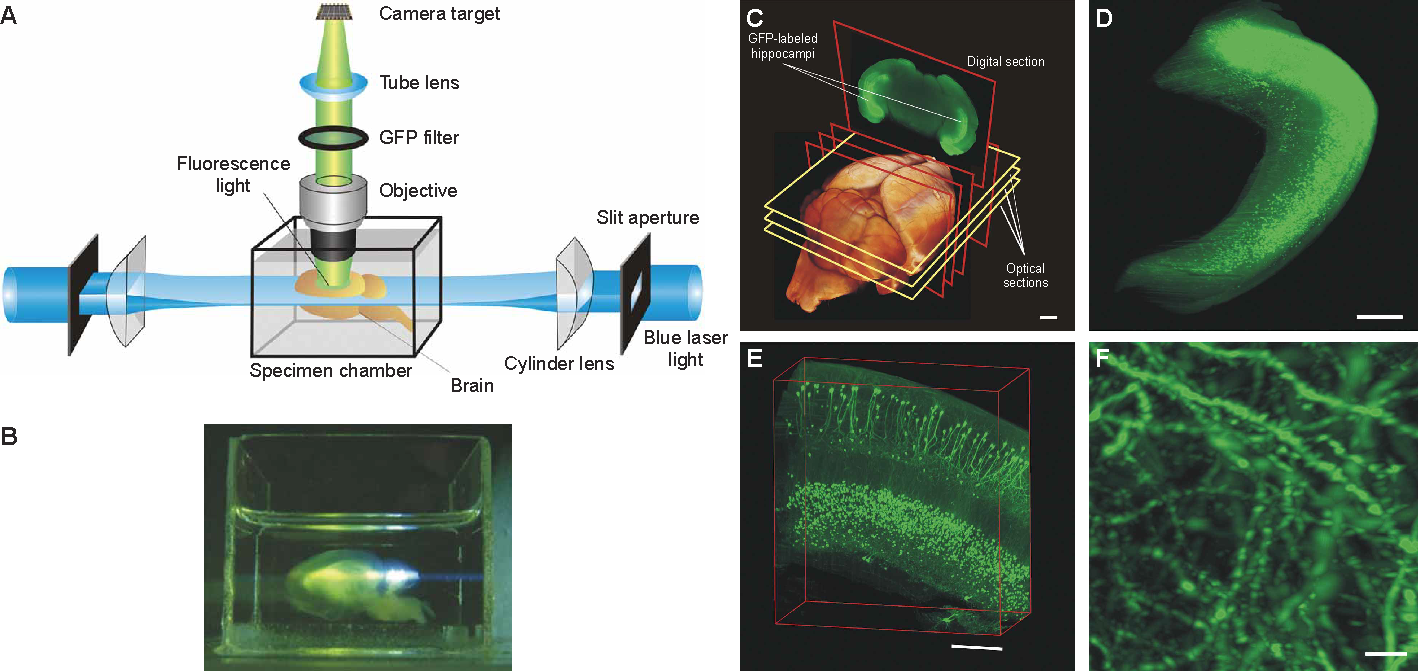
\includegraphics[width=0.8\textwidth]{mammals/Figure4}
      \bcaption[Imaging adult mouse brain with light-sheet microscopy.]{(A) Schematics of the ultramicroscope for brain imaging. The specimen is embedded in clearing medium to ensure necessary imaging depth. Illumination is applied from two sides to achieve even illumination for the whole field of view. Light-sheet is generated by a slit aperture followed by a cylindrical lens. The specimen is imaged from the top using wide-field detection method. (B) Photograph of the imaging chamber with a mounted cleared specimen and light-sheet illumination. (C) Surface rendering of a whole mouse brain, reconstructed from 550 optical sections. GFP and autofluorescence signal was recorded. Hippocampal pyramidal and granule cell layers are visible in the digital section. Scale bar: \SI{1}{mm}. Objective: Planapochromat 0.5×. (D) Reconstruction of an excised hippocampus from 410 sections. Note that single cell bodies are visible. Scale bar: \SI{500}{\micro m}. Objective: Fluar 2.5×. (E) 3D reconstruction of a smaller region of an excised hippocampus from 132 sections. Scale bar: \SI{200}{\micro m}. Objective: Fluar 5×. (F) 3D reconstruction of CA1 pyramidal cells imaged with a higher resolution objective (LD-Plan Neofluar 20× NA 0.4) in a whole hippocampus (430 sections). Dendritic spines are also visible, even though usually a higher NA objective (>1.2) is required to visualize these. Scale bar: \SI{5}{\micro m}. Adapted from Dodt \textit{et al.} \cite{dodt_ultramicroscopy:_2007}.}
      \label{fig:adultMouse}
    \end{figure}

    Imaging adult mice is especially interesting for answering neurobiological questions. Since development is over at this stage, the use of an environmental chamber is no longer necessary. The biggest challenge for imaging these samples is their size, as they are centimeters in size instead of less than a millimeter as in the embryonic stage. Furthermore, the tissues of adult mice are much more opaque which severely limits imaging depth. Light-sheet microscopy can already deal with large specimens, however to achieve (sub)cellular resolution for an entire brain for example, multiple recordings have to be stitched together after acquisition \cite{bria_terastitcher_2012}.

    Light scattering and absorption depend on the tissue composition and imaging depth. Especially the brain with a high concentration of lipids in the myelinated fibers pose a real challenge for imaging. Live imaging is usually performed with 2-photon microscopy which can penetrate the tissue up to \SI{800}{\micro m} deep \cite{katona_fast_2012}. Using fixed samples, however, the scattering problem can be eliminated by the use of tissue clearing methods.

    Tissue clearing is a process that removes and/or substitutes scattering and absorbing molecules by a chemical process while keeping the tissue structure intact and preserving fluorescence. The most dominant contributors to these effects are the proteins and lipids. Proteins in the cells locally change the refractive index of the tissue which leads to scattering, while lipids predominantly absorb the light. Clearing methods tackle these problems by chemically removing and substituting lipids by certain types of gel, and immersing the whole sample in a medium with higher refractive index to match the optical properties of proteins. Numerous methods have been developed for tissue clearing, such as ScaleA2 \cite{hama_scale:_2011}, 3DISCO \cite{erturk_three-dimensional_2012,erturk_three-dimensional_2012-1}, SeeDB \cite{ke_seedb:_2013}, CLARITY \cite{chung_clarity_2013}, CUBIC \cite{susaki_whole-brain_2014} and iDISCO \cite{renier_idisco:_2014}.

    The first combination of optical clearing and light-sheet microscopy for whole brain imaging was performed by Dodt \etal using a custom ultramicroscope consisting of two opposing illumination arms and a single detection with an objective from above (\autoref{fig:adultMouse}A). The light-sheets were positioned horizontally, and the cleared samples could be placed in a transparent imaging chamber filled with the clearing medium (\autoref{fig:adultMouse}B). Imaging was performed from both top and bottom after rotating the sample \SI{180}{\degree}. By changing the detection lens, it is possible to adapt the system to different samples: low magnification is capable of imaging the whole brain (\autoref{fig:adultMouse}C), while for smaller, dissected parts, such as the hippocampus, higher magnification with higher resolution is more appropriate (\autoref{fig:adultMouse}D). With this configuration individual cell-cell contacts can be recognized (\autoref{fig:adultMouse}E), and even dendritic spines can be visualized (\autoref{fig:adultMouse}F).

    Although light-sheet microscopy is highly suitable for imaging cleared specimens, even entire mice \cite{tainaka_whole-body_2014}, brain imaging in live animals is more challenging due to the standard two-objective setup of a conventional SPIM microscope. Two light-sheet-based methods, however offer a solution for this, axial plane optical microscopy (APOM) \cite{li_axial_2014} and swept confocally-aligned planar excitation (SCAPE) \cite{bouchard_swept_2015} both use only a single objective to generate a light-sheet and detect the fluorescence as well. This is done by rotating the detection plane at an intermediate image (APOM), or by rotating both the light-sheet and detection plane simultaneously (SCAPE).




% !TEX root = dissertation_BB.tex
%% spellcheck-language en-US

%  ####
%      #
%   ###
%      #
%  ####

\chapter{Image processing for multi-view microscopy}
  \graphicspath{{./figures/3_processing/}}

  When using any kind of microscopy in research, image processing is a crucial part of the workflow. This is especially true for light-sheet microscopy, since it's capable imaging the same specimen for multiple days, producing immense amounts of data. A single overnight experiment of \textit{Drosophila} development (which is a very typical use-case for light-sheet) can produce multiple terabytes of data. To see the real scales, let's consider the following imaging conditions:
  \begin{center}
  \begin{tabular}{rl}
      camera & Hamamastu Orca Flash 4 \\
      image size & 8 MB \\
      1 stack = 250 planes & 2 GB \\
      2 views & 4 GB \\
      Time-lapse: 16 h @ 2/min & 7.5 TB \\
      $n$ colors & $n\cdot 7.5$ TB
  \end{tabular}
  \end{center}

  As it is apparent from this table, 
  % proportional to the symbol frequencies. A string of symbols can be encoded by applying this process recursively: The sub-interval from the previous step is subdivided again using the same proportions. Figure4.2. shows an example of arithmetic coding using

\section{Multi-view image fusion}
  \subsection{Registration}
    \subsubsection{Image based registration}
    \subsubsection{Bead based registration}
  \subsection{Transformation}
    \subsubsection{Rigid}
    \subsubsection{Affine}
    \subsubsection{Elastic}
  \subsection{Image fusion}
      \subsubsection{Average}
    \subsubsection{Sigmoidal weighted average}
    \subsubsection{Fourier mixing}
    Huisken had something like this
    \subsubsection{Wavelet-based fusion}
    \subsubsection{Multi-view deconvolution}
    
    \cite{krzic_multiple-view_2009} Uros thesis
    \cite{temerinac-ott_multiview_2012}, \cite{temerinac-ott_spatially-variant_2011} Spatially variant deconvolution



\section{Image compression}
  Image compression is an important tool for everyday life, however it's rarely used in the context of scientific imaging because of fear of information loss. This preconception is mainly due to the famous blocking artifacts found in many highly compressed JPEG images, however not all image compression algorithms introduce artifacts, and in fact many lossless algorithms exist that would be suitable for such images. Nowadays, when data production is in an exponential growth compression is again in highlight, without it it would be extremely difficult to maintain many scientific projects that produce images at a high data rate. 

  In this paper I will review the basics of image compression based on Sayood's textbook, Introduction to Data Compression \cite{sayood_introduction_2012}. 
  I will introduce some basics of information theory and entropy, followed by discussing two widely used entropy coding algorithms, Huffman coding and arithmetic coding. Section 3 will be about transform coding, specifically Discrete Cosine Transform (DCT) and wavelet transform while also touching upon techniques based on differential pulse code modulation. Finally I will show how some of the most widely used image compression standards use these methods to achieve effective image compression.

  \subsection{Entropy coding}
    \subsubsection{Information and Entropy}
      "For the purpose of data compression it is useful to quantify the amount of \textit{information} contained within a piece of data. The first rigorous definition of information was presented in an extremely influential paper by Shannon, published in two parts in 1948 \cite{shannon_mathematical_1948, shannon_mathematical_1948-1}."

      "First, let's define the amount of self-information contained in the outcome of a random experiment:"
      \begin{equation}
        I(A) = \log_b \frac{1}{P(A)} = - \log_b P(A)
      \end{equation}

      2 independent events:
      \begin{equation}
        P(A,B) = P(A) \cdot P(B)
      \end{equation}

      self-information is additive:
      \begin{align}
        I(A,B) &= \log_b \frac{1}{P(A,B)} \\
        &= \log_b \frac{1}{P(A) \cdot P(B)} \\
        &= \log_b \frac{1}{P(A)} + \log_b \frac{1}{P(B)}
      \end{align}

      entropy for random variable $X$ ~ average or expected self-information for the random variable
      \begin{equation}
        H(X) = \sum_i P(A_i)I(A_i) = - \sum_i P(A_i) \log_b P(A_i)
      \end{equation}

      entropy rate for data source $S$ ~ average information output by the data source

    \subsubsection{Huffman coding}
      Huffman coding is a prefix-free, optimal code that is widely used in data compression. It was developed by David A. Huffman as a course assignment on the first ever course on information theory at MIT, and was published shortly afterwards \cite{huffman_method_1952}. It is a variable length binary code which assigns different length codewords to letters of different probabilities. It is able to achieve optimal compression, which means the total length of the coded sequence will be minimal.

      Although it produces a variable length code which can introduce some issues with decoding, it is still uniquely decodable. It achieves this property by using prefix-free codewords, meaning that none of the codewords are prefixes of any other codewords. This property can be exploited when decoding the codeword, since during this procedure the number of bits for the next codeword can not be determined in advance. However if no codeword is a prefix of another codeword, by simply reading the successive bits one by one until we reach a valid codeword, it's possible to uniquely decode the message.

      Let's take the example in Table \ref{tab:huffman1}. Five letters are coded in binary code by Code \#1 and by Code \#2. Code 1 is not a prefix code, and because of this when reading the encoded sequence we can not be sure when we reach the end of a codeword. Decoding the sequence 0000 for example could be interpreted as 4 letters of $a_1$ or 2 letters of $a_3$.

      \begin{table}
        \bcaption[Examples of a random binary code (\#1) and a prefix-free binary code (\#2)]{Code \#2 is uniquely decodable, while for code \#1 it's necessary to introduce boundaries between codewords to be able to distinguish them.}
        \centering
        \begin{tabular}{crr}
          \toprule
          Letter & Code \#1 & Code \#2 \\
          \midrule
          $a_1$ & 0	& 10 \\
          $a_2$ & 11	& 11 \\
          $a_3$ & 00	& 00 \\
          $a_4$ & 10 	& 010 \\
          $a_5$ & 111	& 011 \\
          \bottomrule
        \end{tabular}
        \label{tab:prefix}
      \end{table}

      The Huffman coding procedure is based on two observations regarding optimal and prefix-free codes:
      \begin{enumerate}
        \item For a letter with higher frequency the code should produce shorter codewords, and for letters with lower frequency it should produce longer codewords.
        \item In an optimum code, the two least frequent codewords should have the same lengths.
      \end{enumerate}

      From these statements the first is trivial to see that is correct. If the more frequent letters would have longer codewords then the less frequent letters, the average codeword length (weighted by the probabilities) would be larger than in the opposite case. Thus, more frequent letters must not have longer codewords than less frequent letter.

      The second statement at first glance might not be so intuitive, so let's consider the following situation. The two least frequent codewords do not have the same lengths, that is the least frequent is longer. However, because this is a prefix code, the second longest codeword is not a prefix of the longest codeword. This means, if we truncate the longest codeword to the same length as the second longest, they will still be distinct codes and uniquely decodable. This way we have a new coding scheme which requires less space on average to code the same sequence as the original code, from which we can conclude the original code was not optimal. Therefore, for an optimal code, statement 2 must be true.

      \begin{table}
        \bcaption[Huffman code table]{}
        \centering
        \begin{tabular}{ccr}
          \toprule
          Letter & Probability & Codeword \\
          \midrule
          $a_2$ & 0.4 & $c(a_2)$ \\
          $a_1$ & 0.2 & $c(a_2)$ \\
          $a_3$ & 0.2 & $c(a_2)$ \\
          $a_4$ & 0.1 & $c(a_2)$ \\
          $a_5$ & 0.1 & $c(a_2)$ \\
          \bottomrule
        \end{tabular}
        \label{tab:huffman1}
      \end{table}

      \begin{figure}
        \centering
        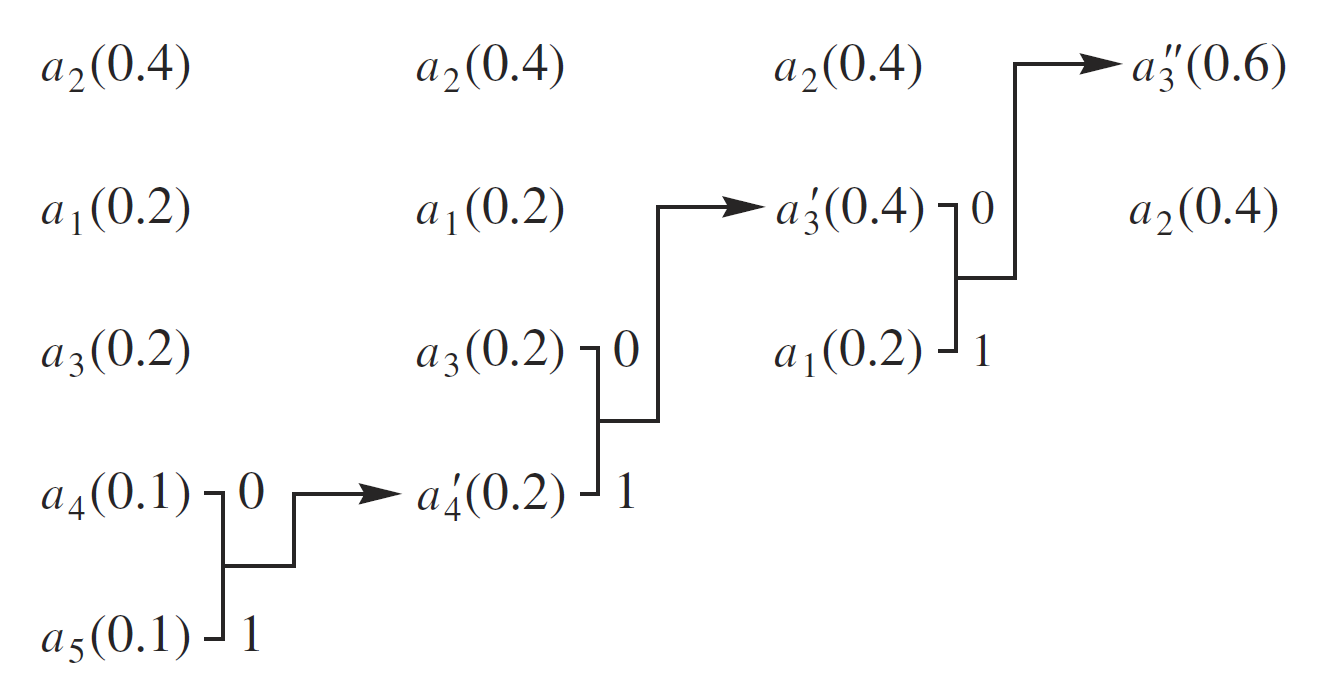
\includegraphics[width=0.6\textwidth]{huffman}
        \bcaption[Building the binary Huffman tree]{The letters are ordered by probability, these will be the final leave of the tree. To join the to branches at every iteration we join the to nodes with the smallest probability, and create a new common node with the sum of the probabilities. This process is continued until all nodes are joined in a root node with probability of 1. Now, if we traverse down the tree to each leaf, the codeword will be defined by their position.}
        \label{fig:huffman}
      \end{figure}

      To construct such a code, the following iterative procedure can be used. Let's consider an alphabet with five letters $A = [a_1,a_2,a_3,a_4,a_5]$ with $P(a_1)=P(a_3)=0.2$, $P(a_2)=0.4$ and $P(a_4)=P(a_5)=0.1$ (Table \ref{tab:huffman1}). "The entropy for this source is 2.122 bits/symbol." Let's order the letters by probability, and consider the two least frequent. Since the codewords assigned to these should have the same lengths, "we can assign their codewords as"
      \begin{align*}
        c(a_4) &= \alpha_1 * 0 \\
        c(a_5) &= \alpha_1 *1
      \end{align*}

      where $c(a_i)$ is the assigned codeword for letter $a_i$ and $*$ denotes concatenation. Now we define a new alphabet $A'$ with only four letters $a_1, a_2, a_3, a'_4$, where $a'_4$ is a merged letter for $a_4$ and $a_5$ with the probability $P(a'_4) = P(a_4) + P(a_5) = 0.2$. We can continue this process of merging the letters until all of them are merged and we have only one letter left. Since this contains all of the original letters, its probability is 1. We can represent the end result in a binary tree (see Figure \ref{fig:huffman}), where the leaves are the letter of the alphabet, nodes are the merged letters, and the codewords are represented by the path from the root node to each leaf (compare with Table \ref{tab:huffman2}). "The average length of this code is"
      \begin{equation}
        l = 0.4\times 1 + 0.2 \times 2 + 0.2 \times 3 + 0.1 \times 4 + 0.1 \times 4 = 2.2 \text{ bits/symbol}
      \end{equation}
      "A measure of the efficiency of this code is its redundancy—the difference between the entropy and the average length. In this case, the redundancy is 0.078 bits/symbol. The redundancy is zero when the probabilities are negative powers of two."

      \begin{table}
        \bcaption[Huffman code table]{}
        \centering
        \begin{tabular}{ccr}
          \toprule
          Letter & Probability & Codeword \\
          \midrule
          $a_2$ & 0.4 & 1 \\
          $a_1$ & 0.2 & 01 \\
          $a_3$ & 0.2 & 000 \\
          $a_4$ & 0.1 & 0010 \\
          $a_5$ & 0.1 & 0011 \\
          \bottomrule
        \end{tabular}
        \label{tab:huffman2}
      \end{table}


    \subsubsection{Arithmetic coding}
      Although in this case the redundancy of the Huffman code is minimal, however in cases where a few symbols have vary high probability compared to the rest, the redundancy increases. This is simply because even for the most frequent letter the shortest codeword the Huffman code can produce is of length 1.

      Let's consider the following example: take alphabet $A=[a_1, a_2]$ with $P(a_1) = 0.95$ and $P(a_2) = 0.05$. The first order entropy for this source is $-0.95 \log 0.95 - 0.05 \log 0.05 = 0.2864$ bits/symbol, however if we assign the Huffman code we will have to use $c(a_1)=0$ and $c(a_2)=1$, which means the average length will be 1 bit/symbol. This means in order to code this sequence using a Huffman code, we will need more than 3 times the number of bits promised by the entropy.

      To get around this fundamental limitation, a coding scheme must be used which does not use discrete codewords at all. Arithmetic coding is the most well-known example of such a scheme. The idea is due to Peter Elias. He developed it during the same course on information theory in which Huffman developed his coding method, but he never published it.

      "In order to distinguish a sequence of symbols from another sequence of symbols we need to tag it with a unique identifier. One possible set of tags for representing sequences of symbols are the numbers in the unit interval [0,1). Because the number of numbers in the unit interval is infinite, it should be possible to assign a unique tag to each distinct sequence of symbols. In order to do this, we need a function that will map sequences of symbols into the unit interval."

      "A straightforward algorithm to arithmetically encode a given input string is the following: Partition the unit interval [0, 1) into sub-intervals and assign one subinterval to each symbol in the input alphabet. The sizes of the sub-intervals are chosen to be proportional to the symbol frequencies. A string of symbols can be encoded by applying this process recursively: The sub-interval from the previous step is subdivided again using the same proportions. Figure \ref{fig:arithmetic}. shows an example of arithmetic coding using the symbol frequencies given in Table \ref{tab:arithmetic}."

      \begin{table}
        \bcaption[Example alphabet for arithmetic coding]{}
        \centering
        \begin{tabular}{cc}
          \toprule
          Letter & Probability \\
          \midrule
          $a_1$ & 0.7 \\
          $a_2$ & 0.1 \\
          $a_3$ & 0.2 \\
          \bottomrule
        \end{tabular}
        \label{tab:arithmetic}
      \end{table}

      \begin{figure}
        \centering
        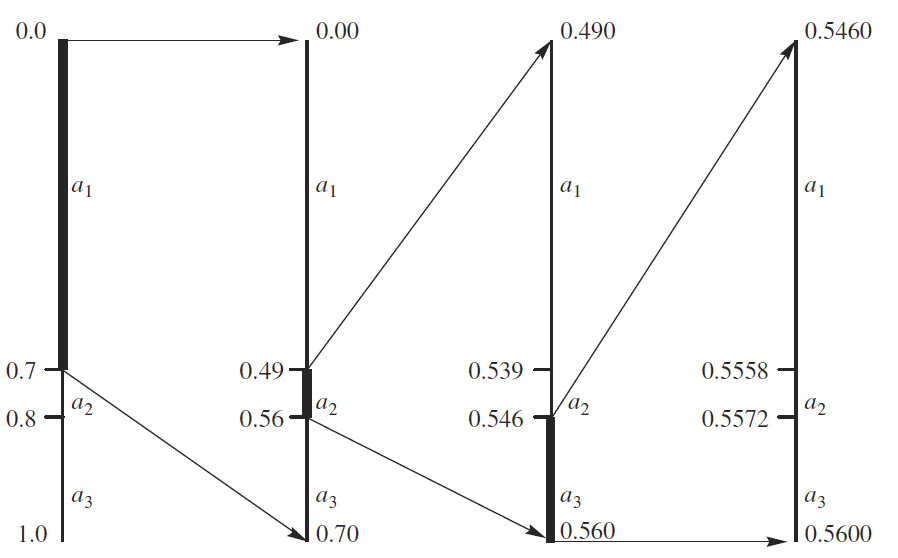
\includegraphics[width=0.6\textwidth]{arithmetic}
        \bcaption[Arithmetic coding scheme in practice with the alphabet from Table \ref{tab:arithmetic} on the sequence $a_1,a_2,a_3$]{}
        \label{fig:arithmetic}
      \end{figure}

      This kind of coding although easy to understand, it's actually quite cumbersome to directly implement on a computer, where only a certain floating point precision can be achieved. For real life use this precision is often unsatisfactory, so some extra steps are involved in the coding.

      Since after each step the next subinterval is a subset of the previous interval, if the coding interval after a certain number of steps is contained in either the upper or lower half of the unit interval it will remain there for the rest of the coding. We can exploit this fact by rescaling that interval to the unit interval and writing either a 0 or 1 bit to the output depending on the position of the subinterval. By continuing this scheme it's possible to reach arbitrary precision even using a computer.

      The decoding process is analogous to encoding. The decoder keeps track of the current lower and upper bounds. It mimics the rescaling operations of the encoder based on the bits of the encoded binary number.

  \subsection{Transform coding}
    The methods outlined in the previous section are effective at compressing the data in an optimal way and reaching the first order entropy, however the assume nothing about the structure of the data. For image compression it's important to also consider this, since most images have a relatively high level of autocorrelation, meaning that neighboring values have a high chance of being similar, although not necessarily equal. Transform coding is a technique that by itself does not compress the data, however by exploiting some knowledge of the structure it transforms the data effectively reducing it's first order entropy. When regular entropy coding is then preformed on the transformed data, because of the reduced first-order entropy, these techniques can achieve a higher rate of compression. At decompression, after decoding the entropy coder, the reverse transformation is applied to reveal the original data. This section will introduce two of the most important algorithms for transform coding, Discrete Cosine Transform and Discrete Wavelet Transform.

    \subsubsection{Discrete Cosine Transform}
      Discrete Cosine Transform \cite{ahmed_discrete_1974} is closely related to the well known Fourier transform. The main idea behind this is to represent a function by a weighted sum of different sine and cosine functions. This provides a different view, instead of looking at the data in the time domain, we gain information about the frequencies that compose the signal. 

      "Discrete Cosine Transform is a variant of the discrete Fourier transformation", however instead of making the signal periodic which can introduce large jumps at the edges, the signal is extended in a symmetric way. Since this will give a smooth transition even at the boundaries, the transform does not have to include so many high frequency components. Also, because of the symmetric extension, it's possible to represent the functions only by using the cosine bases, resulting in fewer coefficients. Overall, the DCT is much better suited for compression, than DFT.

      The DCT base functions are defined in the following way:
      \begin{equation}
      c_{i,j} = s_i \cdot \cos \frac{(2j+1)i\pi}{2n} \qquad \text{with } s_i = 
          \begin{cases}
            \sqrt{\frac{1}{n}} & \text{if } i=0 \\
            \sqrt{\frac{2}{n}} & \text{otherwise}
          \end{cases}
      \end{equation}
      "The scaling factors is are chosen so that the $L_2$ norm of each basis vector is 1 and so the transform is orthonormal. The inverse transform can therefore be found by simply transposing the transform matrix."

      \begin{figure}
        \centering
        
\includegraphics[width=0.4\textwidth]{DCT_bases}
        \bcaption[Basis functions of the $8 \times 8$ 2D DCT, computed as the outer product of the 1D basis vectors.]{}
        \label{fig:DCT_bases}
      \end{figure}

      Applying the DCT to two dimensional functions, i.e. images is very similar to the two dimensional Fourier transform. The base functions are the outer products of the 1D base functions (Figure \ref{fig:DCT_bases}.), and the transform can actually be performed separately for each dimension.

      Computation effort in a naive implementation is $O(n^2)$ but since DCT is based on the Fourier transform, an $O(n \log n)$ algorithm is also possible, analogous to the fast Fourier transform. This is still larger than a linear scaling with the data size, which can be very inconvenient. Therefore, in practice the DCT is usually applied to smaller blocks of the image, such as $4\times4$, $8\time8$ or $16\times16$. 

      Although DCT is an effective way of reducing the first-order entropy, it has a potential shortcoming by its use of floating point arithmetic. Because of the finite machine precision inherent rounding errors will occur, which means the reverse transformation can not generate the exact original data. For many application, such as photography, this still can be acceptable, but for scientific image data lossy compression is generally not accepted.

      DCT-like integer-based variants in JPEG-XR, and H.264


    \subsubsection{Discrete Wavelet Transform}
      "!!CHANGE THIS!!Methods based on Fourier analysis, such as the DCT introduced in the previous section, give excellent localization in frequency space: They tell us exactly which frequencies occur in the data, which is very useful for data compression. However, they give no spatial localization: They do not tell us where in the signal these frequencies occur. Every DCT base function affect the whole image domain!!UNTIL HERE!!"
      , which means distinct local structures can have a global effect on the final outcome. In case of an edge for example, it's necessary to include a high frequency component with a large coefficient, but since every DCT base function has an impact on the whole domain, this will have to be compensated on smoother regions by also increasing the coefficients of other factors. This can negatively impact compression performance.

      A solution for this is to use different base functions, namely ones with finite support. This way we will not only be able to get information about the frequency, but also about the localization of that frequency in some extent.

      "!!!!One option for such a set of local basis functions, and certainly the most popular one, is the multi-resolution analysis based on wavelets. The term “multi-resolution analysis” in the context of wavelets was introduced in the late 1980s by Stéphane Mallat \cite{mallat_theory_1989}, though research on wavelets had been ongoing for several years before that.!!!!"

      "The idea behind the wavelet multi-resolution analysis is to build a basis out of translated and scaled versions of one underlying function called the \textit{mother wavelet} $\psi$. The mother wavelet is non-zero only in a small region, leading to the locality properties. It is translated to cover the whole domain. It also covers only a small frequency band, and is scaled to cover higher or lower frequencies. The family of translated and scaled functions $\psi_{l,i}$ is generated from   according to"
      \begin{equation}
        \psi_{l,i}(t) = \sqrt{2^l} \psi \left(2^l t-i\right), \qquad l, i \in \mathbb{Z}
      \end{equation}
      "Incrementing $l$ halves the width of the resulting function, which thus corresponds to a higher frequency band. Changing $i$ moves the function along the x axis. The size of each step scales with the width of the function, defined by $l$. The normalization factor $\sqrt{2^l}$ is chosen so that the $L_2$ norm stays constant. The mother wavelet can be chosen so that the $\psi_{l,i}$ are pairwise orthogonal and thus form a basis of some function space. However, representing a function in this basis will generally require an infinite number of basis functions $\psi_{l,i}$: To represent a constant component, i.e. content of frequency zero, the wavelet must be infinitely scaled. To address this, it is necessary to introduce an additional scaling function $\phi$ which complements the wavelet. It is scaled and translated the same way as the mother wavelet."

      The oldest wavelets are the Haar wavelets, and because of their simplicity, they provide a good example on how wavelet transformation works. The Haar wavelet scaling $\phi$ and wavelet $\psi$ functions are the following:
      \begin{equation}
        \phi(t) = 
        \begin{cases}
          1 & \text{if } 0 \leq t < 1 \\
          0 & \text{otherwise}
        \end{cases}
        \label{eq:scaling}
      \end{equation}

      \begin{equation}
        \psi(t) = 
        \begin{cases}
          -1 & \text{if } 0 \leq t < \frac{1}{2} \\
          1 & \text{if } \frac{1}{2} \leq t < 1 \\
          0 & \text{otherwise}
        \end{cases}
        \label{eq:wavelet}
      \end{equation}
      "Clearly, all wavelet functions $\psi_{l,i}$ are orthogonal. Additionally, the scaling functions $\phi_{l,i}$ at a fixed level $i$ are orthogonal. The scaling functions $\phi_{l,i}$ are also orthogonal to the wavelet functions $\psi_{k,i}$, $k \geq l$ at the same and all finer levels."

      "Figure \ref{fig:wavelet}. (left) schematically shows the decomposition of a signal into low-pass components corresponding to the scaling function, and high-pass components corresponding to the wavelet. The signal $s_0$ can be represented by the translated scaling function at a finer scale $l_0$, "which can be decomposed to the sum of a coarser approximation $s_1$ corresponding to the scaling function and the detail part $d_1$ corresponding to the wavelet functions. This decomposition to a sum of coarser approximation and detail can be continued multiple times, thus resulting in the previously mentioned multi-resolution analysis.


      \begin{figure}
        \centering
        "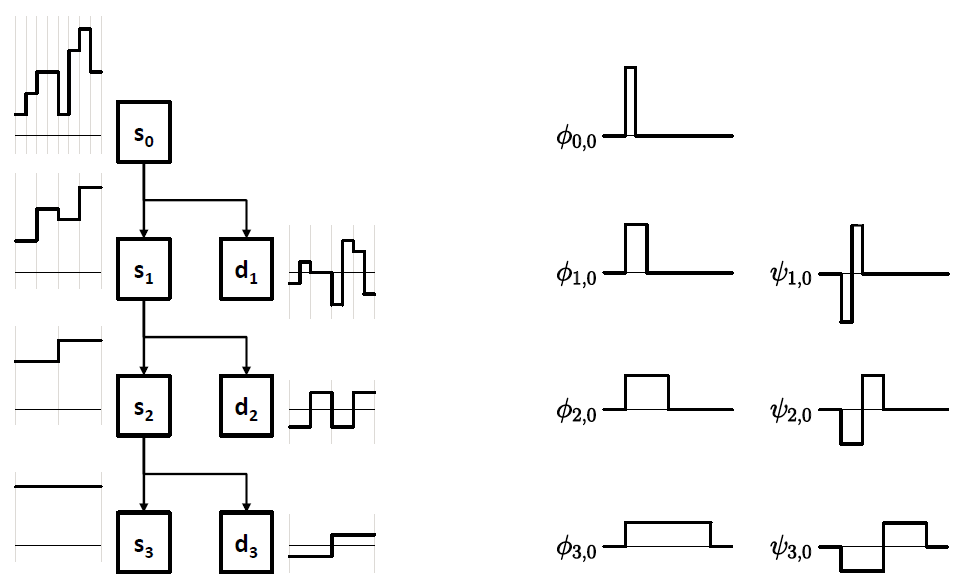
\includegraphics[width=0.6\textwidth]{wavelet}"
        \bcaption[Multi-resolution wavelet decomposition, using the Haar wavelets as an example]{Left: decomposition to multiple levels of low pass and high pass coefficients corresponding to the scaling and the wavelet functions respectively. Right: some of the base wavelet functions used for the decomposition.}
        \label{fig:wavelet}
      \end{figure}


      Of course, for image compression applications, it is desirable to extend this transformation to a 2D version, that can be applied to the images before performing the arithmetic coding. Similarly to the DCT, the wavelet transform is also separable, and can be performed as a sequence of 1D transforms along different directions. Separable in a sense, that it does not matter in which order the individual 1D DWTs are applied to get the same 2D transformation.

      JPEG \cite{pennebaker_jpeg:_1992}, JPEG-LS \cite{weinberger_loco-i_2000} and JPEG2000

  \subsection{Differential pulse code modulation / LOCO-I?}

  

  % \section{Conclusion}
  % In this paper I have introduced some of the most important techniques for image compression. Many of these are used in different image compression algorithms, such as . The common point for each of these formats is that they first transform the images to effectively reduce first order entropy, either by predicting the pixel values and coding only the differences (JPEG-LS), or by using either Discrete Cosine Transform (JPEG) or Discrete Wavelet Transform (JPEG2000). In the case of lossy standards after this transformation step a quantization is also performed depending on the desired quality setting for the coder. Finally as the last step the transformed and quantized coefficients are compressed by an arithmetic coder, such as Huffman coding in JPEG of arithmetic coding in JPEG2000. The end result in each case is a highly optimized compression that greatly reduces the file size.

\section{Noise in light microscopy images}
  \subsection{Photon shot noise}
  \subsection{Camera noise}
    \subsubsection{CCD}
    \subsubsection{EM-CCD}
    \subsubsection{sCMOS}
  \subsection{Variance stabilization}



% !TEX root = dissertation_BB.tex
%% spellcheck-language en-US

%  ####
%      #
%   ###
%  #
%  #####

\chapter{Dual Mouse-SPIM}

\graphicspath{{./figures/2_DualMouse/}}

% \section{Challenges in imaging mouse pre-implantation development}
  % mammalian development
  % chromosome segregation
  % cell specification
  % symmetry breaking
  % signaling pathways
  % human infertility
  % congenital diseases 

  % advantages:
  %   immersion liquid and culture medium separated
  %   open-top sample holder allow standard microdrop \textit{in vitro} embryo culture
  %   row of embryos - high throughput
  %   dual color imaging
  %   environmental chamber allows live imaging for 3 days, every 

  % follow chromosomes by tracking kinetochores

  % from lattice paper: ``because photodamage mechanisms that scale supralinearly with peak intensity have been identified for both visible \cite{donnert_major_2007} and two-photon \cite{ji_high-speed_2008} excitation."


  As we have seen in the previous chapter, live imaging of mouse embryonic development is an especially challenging task, but light-sheet microscopy can offer a good solution owing to its gentle optical sectioning, and fast image acquisition. The mouse SPIM introduced in the previous chapter also solves the issue of live imaging with its inverted design: the embryos are held by a foil that not only allows easy sample handling, but also acts as a barrier, and isolates the embryos from the immersion medium.

  As all microscopes, the mouse SPIM also had to make a compromise: although its design allows long term live imaging, it only has a single detection view, as rotation is not possible with the sample mounting trays. Due to this configuration, its resolution is inherently anisotropic, having an axial to lateral resolution ratio of around 3. Although this is sufficient for many applications, such as cell tracking, for detecting subcellular features it might be limiting. One such application is chromosome tracking, which could shed light on chromosome missegregation mechanisms in the early embryonic development, which is the cause of many congenital diseases also affecting humans.

  In this chapter, we describe a novel light-sheet microscope developed to address the above challenges by using high NA objectives for subcellular isotropic resolution and low-light imaging, and offering multi-view detection without having to rotate the samples. The microscope is designed to be live imaging compatible, offering new perspectives in the research of mouse embryonic development. This chapter will describe the design considerations for the microscope, the optical layout, alignment strategies, and the result of various performance measurements, and its multi-view imaging capabilities. 

  %#######  ########  ######  ####  ######   ##    ## 
  %#     ## ##       ##    ##  ##  ##    ##  ###   ## 
  %#     ## ##       ##        ##  ##        ####  ## 
  %#     ## ######    ######   ##  ##   #### ## ## ## 
  %#     ## ##             ##  ##  ##    ##  ##  #### 
  %#     ## ##       ##    ##  ##  ##    ##  ##   ### 
  %#######  ########  ######  ####  ######   ##    ## 

\section{Microscope design concept}
\label{sec:120concept}

  \begin{figure}
    \centering
    \begin{subfigure}{0.49\textwidth}
      \centering
      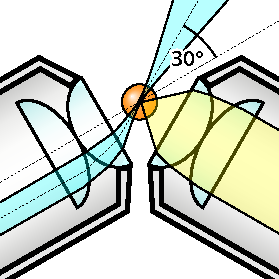
\includegraphics[page=1,width=0.8\textwidth]{objectiveCloseup}
    \end{subfigure}
    \begin{subfigure}{0.49\textwidth}
      \centering
      \includegraphics[page=2,width=0.8\textwidth]{objectiveCloseup}
    \end{subfigure}
    \bcaption[Dual view concept with high NA objectives]{To achieve multi-view detection while maximizing resolution and light collection efficiency, two high NA objectives are placed in \SI{120}{\degree} arrangement. The sample (orange) is held from below by a thin FEP foil. To be able to overlap the light-sheet with the focal plane, the light-sheet is tilted \SI{30}{\degree}. The objectives are used in an alternating sequence for illumination and detection.}
    \label{fig:objectiveCloseup}
  \end{figure}

  As the limiting factor for subcellular imaging with the original mouse-SPIM is the poor axial resolution relative to the lateral, our first aim was to increase the axial resolution to ideally reach the lateral resolution. A common way to reach isotropic resolution is to image a specimen from multiple directions, and combine the resulting images by multi-view deconvolution \cite{swoger_multi-view_2007,temerinac-ott_multiview_2012, preibisch_efficient_2014}. This has the benefit that the high resolution information from the other views can complement the low axial resolution of the first view, thus providing better resolution an all 3 directions.

  As we have seen in the previous chapter, many SPIM implementations allow for recording multiple views either by rotating the sample, or by surrounding the sample with multiple objectives that are used for detection (\autoref{fig:spim_zoo}). For our setup, following the sample mounting technique of the original mouse SPIM, we wanted to keep the open-top sample mounting possibility, as this was proven to be highly compatible with mouse embryo imaging. To be able to achieve multi-view detection in this configuration, we designed a setup where both objectives can be used for illumination and detection in a sequential manner, inspired by previous symmetrical SPIM designs \cite{balazs_development_2013, wu_spatially_2013}.

  To achieve the highest possible resolution from two views, the core of our design is based on the symmetric arrangement of two Nikon CFI75 Apo LWD 25x water dipping objectives, with a numerical aperture of 1.1. Due to the large light collection angle of these objectives, we arrange them in \SI{120}{\degree} instead of the conventional \SI{90}{\degree} used for light-sheet imaging. As the light-sheet still needs to coincide with the imaging focal plane of the objectives, we tilt the light-sheets by \SI{30}{\degree} (\autoref{fig:objectiveCloseup}). Due to the low NA of the light-sheet, this is possible without affecting illumination quality.

  This \SI{120}{\degree} arrangement has several benefits when compared to the traditional \SI{90}{\degree} configuration. When placing the objectives in \SI{90}{\degree}, the largest possible light collection half-angle for an objective can be $\alpha_{max,90} =\SI{45}{\degree}$, and the corresponding NA is $\na_{max,90} = n \cdot \sin \alpha_{max,90} = 0.94$, where $n=1.33$ the refractive index of water. The closest to this from the commercially available objectives offers a numerical aperture of 0.8. For a \SI{120}{\degree} arrangement, the theoretical maximum is $\na_{max,120} = n \cdot \sin (\SI{120}{\degree} /2) = 1.15$.

  Although the resolution won't be completely isotropic when combining the images from two \SI{120}{\degree} views (\autoref{fig:psf-rot}), as it is for \SI{90}{\degree} views, due to the higher maximum NA possible, the resolution can be higher in the \SI{120}{\degree} case. When simulating the combined multi-view PSFs (\autoref{fig:psf-rot}), for NA=0.8 objectives in \SI{90}{\degree} the axial and lateral resolutions are both \SI{317}{nm}; while for two NA=1.1 objectives in \SI{120}{\degree} the axial resolution will be identical, \SI{317}{nm}, and the lateral will be better, at \SI{193}{nm}.
  
  Although this difference in resolution may seem marginal, the \SI{120}{\degree} configuration has a another advantage in light collection efficiency. Collecting as much of the fluorescence signal as possible is crucial in live imaging applications, due to the limited available photon budget (see \autoref{fig:tradeoffs} and \cite{laissue_assessing_2017}). Collecting more light from the sample allows to image faster with the same contrast, or to reduce the illumination power and maintaining the imaging speed. As light collection efficiency depends on the solid angle subtended by the detection lens, (see Appendix \autoref{app:lightEff}), a 1.1 NA objective can collect twice as many photons as a 0.8 NA objective, which gives the \SI{120}{\degree} setup a clear edge in low-light imaging.

  \begin{figure}
    \centering
    \begin{subfigure}[t]{0.45\textwidth}
      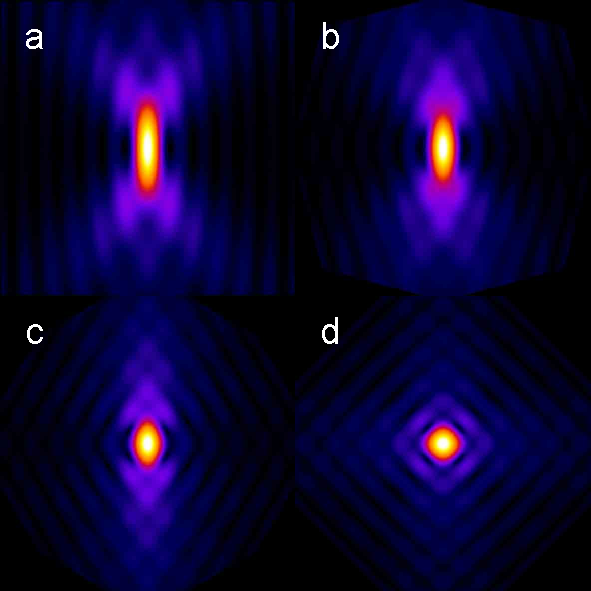
\includegraphics[width=\columnwidth]{simu/psf}
    \end{subfigure}	
    \begin{subfigure}[b]{0.5\textwidth}
    \qquad e
    
      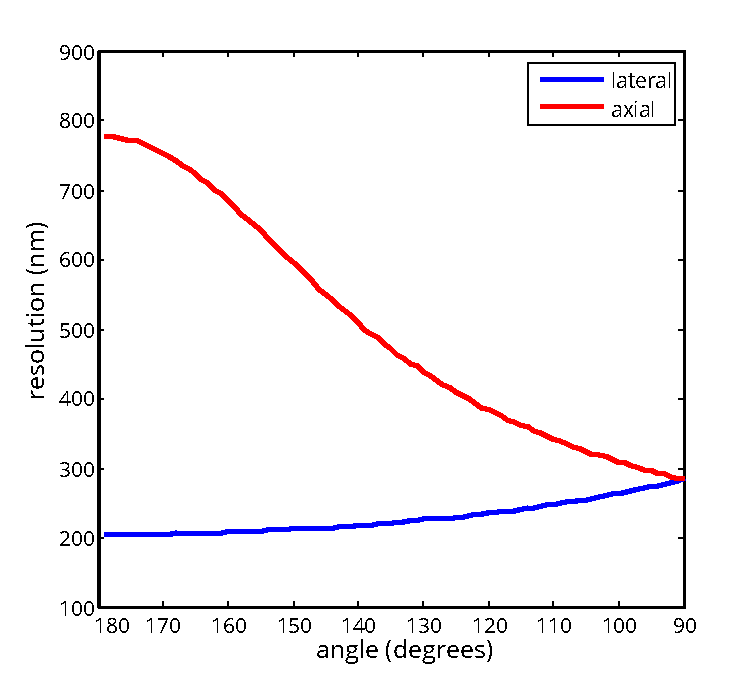
\includegraphics[width=\columnwidth]{simu/resolution}
    \end{subfigure}
    \bcaption[Lateral and axial resolution of a multi-view optical system.]{a) Simulated PSF for a single view. b)--d) Simulated compound PSF of two views aligned in b) 30, c) 60 and d) 90 degrees to each other. e) Axial and lateral resolution of a dual-view setup depending on the rotation angle of the two objectives. Parameters used for calculations: NA=1.1, $\lambda_{ex}=488$nm, $\lambda_{det}=510$nm, $n=1.333$ for water immersion.}
    \label{fig:psf-rot}
  \end{figure}


  % Due to the sample mounting constraints (\autoref{fig:preMouse}) when imaging mouse embryos, it is not feasible to surround the sample with objectives, as it can be done with other specimens, such as a \textit{Drosphila} embryo. Rotation is also not possible, since the sample holder is open on the top. To still allow for multi-view imaging, one possibility is to use two identical objectives, both capable of illumination and detection, in a symmetrical configuration \cite{balazs_development_2013,wu_spatially_2013}

  % In order to address the challenges outlined in the previous section, we propose a new light-sheet microscope design for imaging pre-implantation development at high resolution. The design is guided by the following requirements:
  % \begin{enumerate}
  %   \item subcellular, isotropic resolution
  %   \item high light collection efficiency
  %   \item live embryo compatible
  % \end{enumerate}
    

  \subsection{Light-sheet design}
    \label{sec:ls-design}
    To allow for flexibility in the field of view height, even illumination, reduced stripes, and potential for confocal line detection, we opted to use the beam scanning technique to generate a virtual light-sheet. The effective focal length of the Nikon 25x objective, given the \SI{200}{mm} focal length tube lens is
    \begin{equation}
    f_{o} = \frac{f_{tl}}{M} = \frac{200\text{  mm}}{25} = 8 \text{  mm},
    \end{equation}
    and the back aperture diameter is \SI{17.6}{mm}.
    
    To generate the tilted light-sheet as shown on Fig. \ref{fig:objectiveCloseup}, the illumination beam will need to be displaced by
    \begin{equation}
      \delta = f_o \cdot \tan \SI{30}{\degree} = \SI{4.62}{mm}
    \end{equation}
    
    Since the Gaussian beam is not uniform, only a smaller portion of it can be used to maintain even illumination (\autoref{fig:fov}). Because the size of an early mouse embryo is around \SI{80}{\micro m}, we require the length and the height of the light-sheet to be at least \SI{100}{\micro m}.
    

    \subsubsection{The length and thickness of the light-sheet}
    
      As we saw in \autoref{sec:dimensions}, the length of the light-sheet is determined by the Rayleigh-range of the beam in the $zy$ plane. Since $l_{fov}=2\cdot z_{R}=\SI{100}{\micro m}$
      \begin{equation}
        z_{R}=\SI{50}{\micro m}
      \end{equation}
      Since the Rayleigh range and the diameter of the beam waist are coupled, the light-sheet thickness can be calculated after rearranging \autoref{eq:rayleigh}
      \begin{equation}
        2\cdot W_{0} = 2\cdot \sqrt{\frac{z_R \cdot \lambda}{\pi}} = \SI{5.57}{\micro m}
      \end{equation}
      when $\lambda=\SI{488}{nm}$ for GFP excitation. As the beam width for these calculations is defined as $1/e^2$ of the peak intensity, we also calculate the more commonly used full width at half maximum (FWHM):
      \begin{equation}
        \mathrm{FWHM} = W_0 \cdot \sqrt{2 \ln 2} = \SI{3.28}{\micro m}.
      \end{equation}
      
      From this, the divergence angle of the beam is
      \begin{equation}
        \theta_0 = \frac{\lambda}{\pi W_0,y} = \SI{55.74}{mrad} = \SI{3.196}{\degree}
      \end{equation}
      This means, the numerical aperture needed to produce this light-sheet is:
      \begin{equation}
        \NA_{ls} = n\cdot \sin(\theta _0) = 0.0743
      \end{equation}
      Since $\NA=1.1$, and the diameter of the back aperture is $d=\SI{17.6}{mm}$ and the divergence angle $\theta_0 \ll 1$, using paraxial approximation, the necessary beam width at the back focal plane in the $y$ direction is
      \begin{equation}
        b_y = d \cdot \frac{\NA_{ls}}{\NA} = \SI{1.19}{mm}
      \end{equation}
      Thus, to generate a light-sheet with appropriate length to cover a whole mouse pre-implantation embryo, the laser beam diameter should be $b=\SI{1.19}{mm}$. Larger than this will result in a more focused beam, and a shorter light-sheet, while a smaller diameter beam will have worse optical sectioning capabilities.

    \subsubsection{The height of the light-sheet}
    
    The height can be adjusted by changing the beam scanning amplitude with the galvo mirror. To scan the entire field of view of $h_{fov} \SI{270}{\micro m}$, the scanning angle range at the back focal plane of the objective will need to be $ \theta = \tan^{-1}(h_{fov}/2/f_o) = \pm \SI{0.967}{\degree}$.


      

 %######  ########  ######## ####  ######   ######  
%#     ## ##     ##    ##     ##  ##    ## ##    ## 
%#     ## ##     ##    ##     ##  ##       ##       
%#     ## ########     ##     ##  ##        ######  
%#     ## ##           ##     ##  ##             ## 
%#     ## ##           ##     ##  ##    ## ##    ## 
 %######  ##           ##    ####  ######   ######  

\section{Optical layout}
  
  Based on the requirements and other considerations layed out in the previous section, the microscope was designed based on three main parts: 1) the core unit, 2) illumination and 3) detection branches. The aim when integrating everything together was to allow for high level of flexibility with robust operation, while keeping efficiency at a high level. After finalizing the concept, the optical layout of the microscope was designed in SolidWorks.

  % \begin{figure}[bth]
  %   \centering
  %   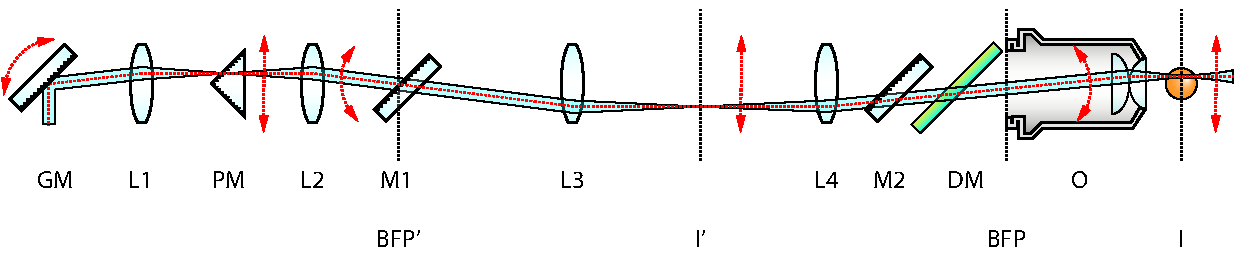
\includegraphics[page=1,width=1\textwidth]{schematicsLinear}
  %   \bcaption[Simplified schematics for illumination]{}
  %   \label{fig:schematicsLinear}
  % \end{figure}


  \subsection{Core unit}
  \label{sec:core}
    \begin{figure}
      \centering
      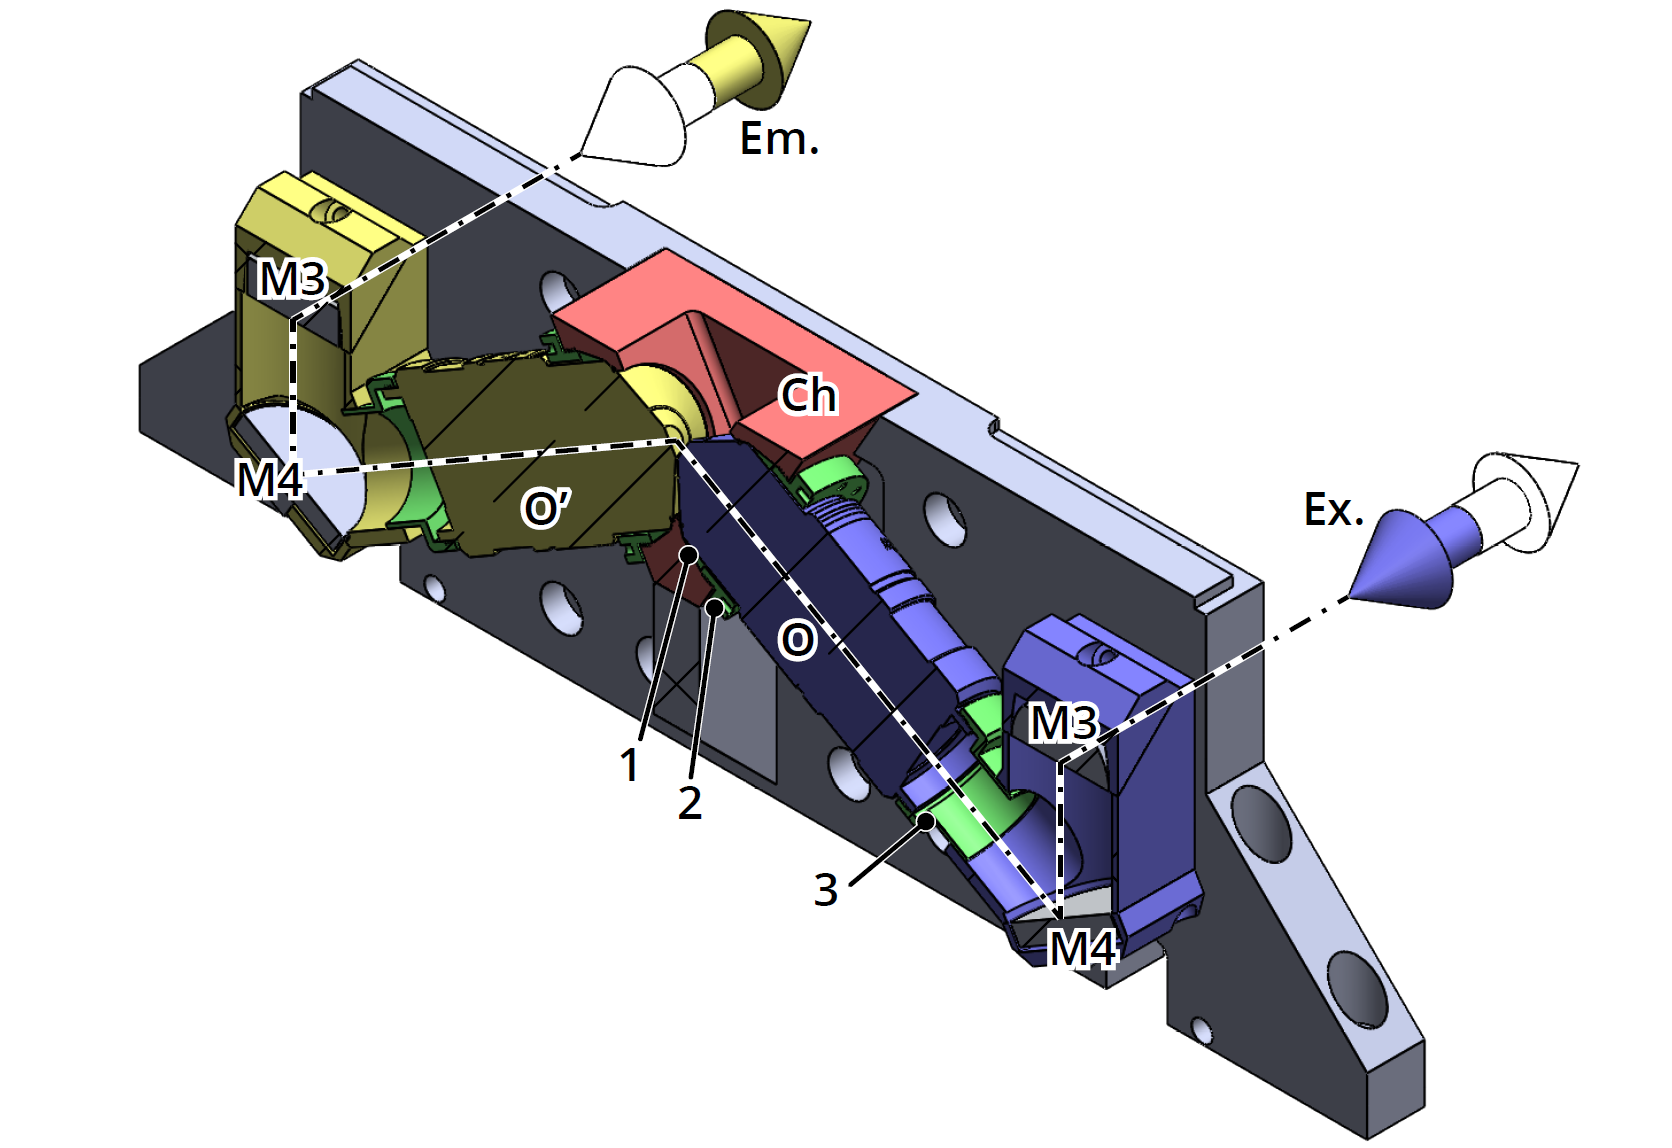
\includegraphics[width=0.8\textwidth]{SW/frontRender.png}
      \bcaption[The core unit of the microscope]{The two objectives (O and O') are mounted on a solid \SI{15}{mm} thick aluminium plate. Fitting on the objectives, a custom chamber (Ch) is holding the immersion medium for imaging. The mirror block with mirrors M3 and M4 directs the light to \SI{65}{mm} optical rails. Excitation (Ex.) and emission (Em.) light paths are indicated by the dash-dot line. Due to the symmetric arrangement, the excitation and illumination paths can be switched around. Objectives are secured with rings 1--3 (green, see main text for details).}
      \label{fig:Core}
    \end{figure}

    As the most important part of the microscope is actually the sample, the design is based around a core consisting of the imaging chamber and the objectives (\autoref{fig:Core}). Also part of the core are two mirror blocks placed at the back of the objectives, and three custom designed rings to hold the objectives in place. The objectives are pointing slightly up, closing a \SI{60}{\degree} angle with the horizontal plane, and \SI{120}{\degree} angle with each other. 

    \subsubsection{Chamber}
    The chamber serves two purposes: it holds the immersion liquid necessary for imaging, and it also keeps the objectives in the \SI{120}{\degree} position. The objectives are held by their necks as opposed to the standard mounting method from the back by the threads. The advantage of this is that any axial movements due to thermal expansion are greatly reduced, thus the focal plane position is more stable even when changing the imaging conditions.

    The chamber is machined form a high performance plastic, poly(ether-ether-ketone) (PEEK). This material has many beneficial properties: it is food safe, and chemically extremely inert, resisting to most solvents used in a biology laboratory. It can also be autoclaved. Compared to other plastics its mechanical properties are also superior. It has high tensile and compressive strength, comparable to aluminium, low thermal expansion and low thermal conductivity. This can be beneficial when implementing temperature control, as thermal loss is reduced.

    The objectives are kept in place by two custom designed rings (\autoref{fig:Core} 1, 2). The first ring has a cross sectional shape of a wedge, and sits tightly against both the objective and the wall of the chamber. The second ring can freely slide on the objective, and has threads matching the chamber. When turned in, the threaded ring pushes the wedge ring further in, which in turn presses against the objective and the chamber wall uniformly, thus preventing the objective from moving, and sealing the chamber at the same time. As the wedge ring is made from a soft plastic (delrin), it will press evenly against the objective preventing any damage. Because of the conical shape of the ring, it will also automatically center the objective, ensuring correct positioning.

    To relieve any rotational stresses from the objective, the back of the objective is also supported  by the mirror block, this is not fixed, however. A third ring, made of PEEK is screwed on the thread of the objective, and slides in the opening of the mirror block. This reduces the torque on the objectives, while still allowing for some movements that might occur due to thermal expansion.

    \subsubsection{Mirror blocks}
    \label{sec:mirrors}
    Apart from supporting the objectives from te back, the mirror blocks are housing two broadband dielectric mirrors (Thorlabs, BBE1-E03 and OptoSigma, TFMS-30C05-4/11) to direct the light in and out from the objectives on a standard \SI{65}{mm} height, compatible with the Owis SYS65 rail system. The combination of two mirrors have two benefits compared to using just one. With a single mirror directly reflecting the light to the back, the entire assembly would need to be much higher to reach the desired \SI{65}{mm} height. This could result in stability problems. Furthermore, due to the \SI{60}{\degree} rotation angle of the objective, the image of the objective would also be rotated if using only a single mirror. With two mirrors the reflection planes can be kept orthogonal to the optical table, which will result in a straight image after the mirror block. This is not only beneficial when recording the images, but also when aligning the illumination arm. With the use of two mirrors, a convenient vertical scanning is required to produce the light-sheet; with a single mirror, the scanning direction would need to be rotated by \SI{60}{\degree}.


  \subsection{Illumination}
    \begin{figure}[bt!]
      \centering
      \begin{subfigure}{\textwidth}
        \centering
        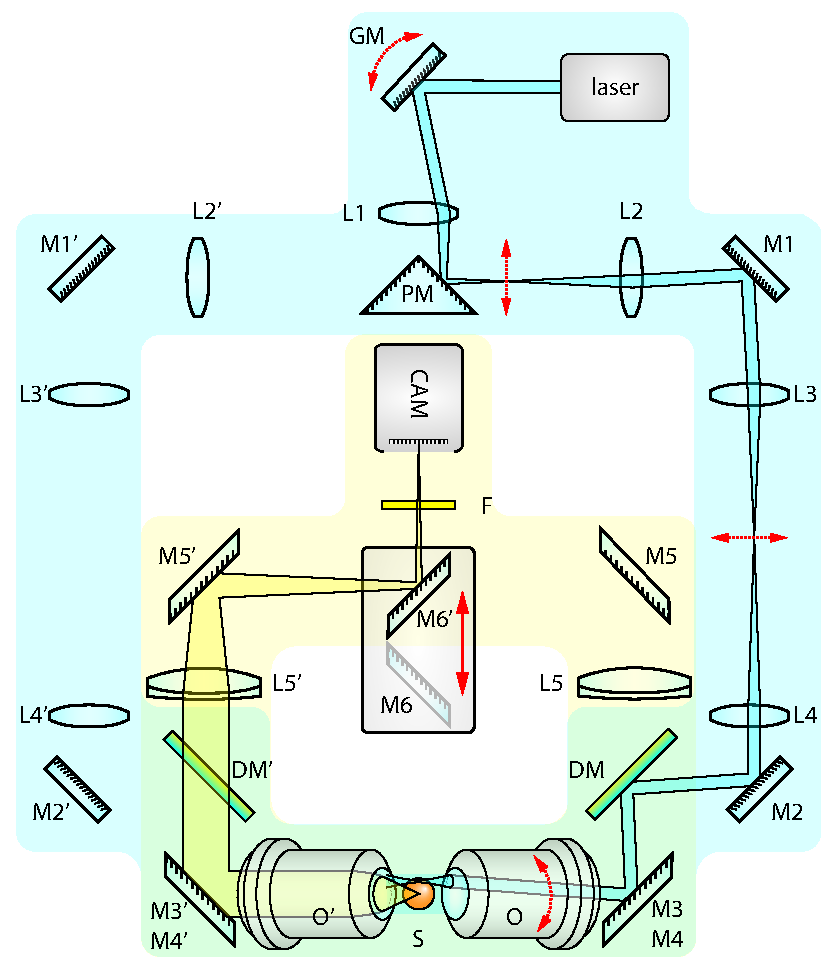
\includegraphics[page=1,width=0.9\textwidth]{fullSchematics}
      \end{subfigure}
      \begin{subfigure}{\textwidth}
        \centering
        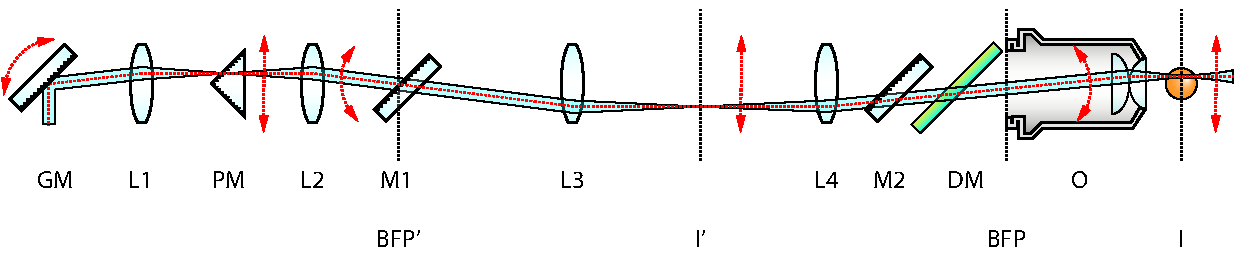
\includegraphics[page=1,width=1\textwidth]{schematicsLinear}
      \end{subfigure}
      
      \bcaption[Dual Mouse SPIM optical layout]{The microscope consists of two main parts, the illumination branches (blue) and detection branches (yellow). For both illumination and detection there are two identical paths implemented. Illumination direction can be changed by applying a different offset to the galvo mirror, which in turn will direct the beam to the opposite face of the prism mirror. L1 and L2 will then image the galvo on M1. Using L3 as a scan lens, and L4 as a tube lens, the scanned beam is coupled to the objective path by quad band dichroic mirror (DM)
      CAM -- camera, DM -- dichroic mirror, F -- filter wheel, L -- lens, M -- mirror, O -- objective, PM -- prism mirror, S -- sample}
      \label{fig:fullSchematics}
    \end{figure}

    The illumination arm of the microscope directs and shapes the laser beam to generate the proper light-sheet dimension at the sample. As was calculated in \autoref{sec:ls-design}, a beam diameter of \SI{1.2}{mm} is ideal for this setup.

    The illumination arm has 3 main roles:
    \begin{enumerate}
      \item expands the laser beam to the calculated \SI{1.2}{mm} size.
      \item images the galvo scanner to the back focal plane of the objective
      \item switches the laser light between the two objectives during imaging
    \end{enumerate}

    To achieve the desired beam diameter, a 1:2 beam expander (Sill Optics, 112751) is used in the reversed direction. As the output of the laser fiber produces a \SI{3}{mm} diameter beam, this will reduce it to \SI{1.5}{mm}. As this is already the required beam diameter, the lenses further in the illumination path will not introduce any magnification.
    
    % \subsubsection{Beam splitter unit}
    \label{sec:splitter}

    Switching between the two illumination arms is performed by a custom designed beam splitter unit (\autoref{fig:splitter}). Instead of utilizing a 50/50 beam splitter cube and mechanical shutters, we exploit the fact that a galvo scanner is needed to generate the light-sheet. As this galvo scanner (Cambridge Technology, 6210B) has a relatively large movement range ($\pm \SI{20}{\degree}$) it is also suitable for diverting the beam from one illumination arm to the other.

    \begin{figure}[htb]
      \centering
      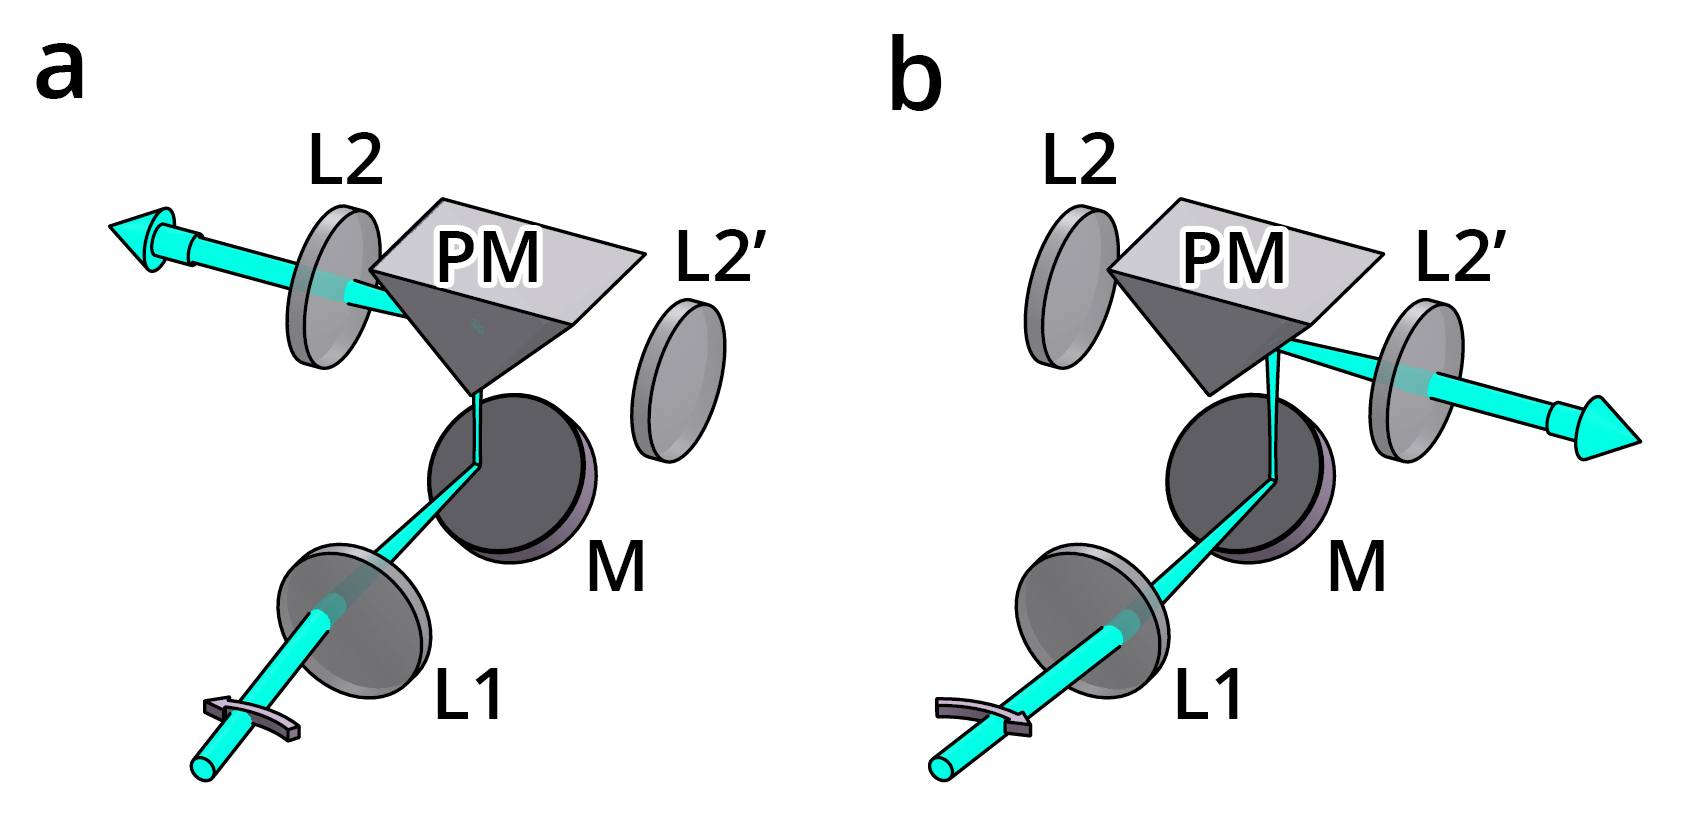
\includegraphics[width=0.8\textwidth]{SW/splitterFigure}
      \bcaption[Illumination branch splitting unit]{To divert the beam to either side, a right angle prism mirror is used in conjunction with a galvanometric scanning mirror. L1 acts as a scan lens, thus the beam is translated on mirror M. Depending on the galvo angle, the beam will be reflected either to the left (\textbf{a}) or to the right (\textbf{b}). L2 and L2' act as relay lenses, and will image the galvo movement to intermediate planes.}
      \label{fig:splitter}
    \end{figure}

    Switching illumination side is done the following way. As the galvo is positioned at the focus of the first lens (L1, $f_1 = \SI{75}{mm}$, Edmunds Optics, \#47-639), the rotational movement will result in a linear scanning movement on mirror M and the prism mirror PM (Thorlabs, MRAK25-E02). Depending on the lateral position of the beam, it will hit either the left or the right leg of the prism, and will be reflected to either direction. As the galvo mirror can be precisely controlled through our custom software, we can set and save the position when the beam is centered on the left lens L2 ($f_2 = \SI{75}{mm}$, Edmunds Optics, \#47-639) (\autoref{fig:splitter}a) and the position when the beam is centered on the right lens L2' (\autoref{fig:splitter}b). Lenses L1 and L2(L2') form a 4f system, and are imaging the galvo scanner on mirror M1(M1') (\autoref{fig:fullSchematics}). This way we can use the same galvo to generate the light-sheet for both directions, depending on the initial offset position. This not only has the advantage of being able to electronically switch the illumination arms, but only requires a single galvo scanner instead of one for each arm.
    
    Due to the arrangement of the bottom mirror and the prism mirror, the scanning direction will be rotated by \SI{90}{\degree}. This will result in a vertical scanning plane, which is exactly what we need to generate the light-sheet on the sample (see \autoref{sec:mirrors}).

    % \subsubsection{the rest of illumination}
    Further following the illumination path, two achromatic lenses L3 and L4 ($f_3 = f_4 = \SI{200}{mm}$), in a 4f configuration relay the scanning axis to the back focal plane (BFP) of the objective. To couple in the laser with the imaging path, a quad-band dichroic mirror (DM, Semrock, Di03-R405/488/561/635-t3-25x36) is used, matching the wavelengths of the laser combiner.

  \subsection{Detection}
    As the emitted light exits the objective and the mirror block, it is decoupled from the illumination path by the dichroic mirror. The light is then focused by a \SI{400}{mm} achromatic lens (L5, Edmunds Optics, \#49-281) onto the camera sensor (Andor Zyla 4.2 sCMOS). Just before the camera, a motorized filter wheel (F, LEP 96A361) is placed to filter out any unwanted wavelength from the emission light. Although this is not in the infinity space, due to the very small angles after the \SI{400}{mm} tube lens, the maximum axial focal shift is $\sim \SI{50}{nm}$ only, which is negligible compared to the axial resolution of $\sim \SI{1.1}{\micro m}$.

    Similarly to the common galvo in the illumination path, the two detection arms share the same camera. Although two cameras could also be used, due to the operating principle of the microscope, the two objective are not used for imaging at the same time. This means a single camera is capable of acquiring all the images, however, the two distinct detection arms need to be merged to be able to use a single camera.
    
    Our solution to this problem is a custom designed view switching unit comprised of two broadband dielectric elliptical mirrors (Thorlabs,BBE1-E03) ) facing opposite directions, mounted on a high precision linear rail (OptoSigma, IPWS-F3090). Depending on the rail position, either the left (\autoref{fig:dualMirror}a) or the right (\autoref{fig:dualMirror}b) detection path will be reflected up, towards the camera. 

    Moving the switcher unit is performed by a small, \SI{10}{mm} diameter pneumatic cylinder (Airtac, HM-10-040) that is actuated by an electronically switchable 5/2 way solenoid valve (Airtac, M-20-510-HN). This solution offers a very fast switching between views, up to \SI{5}{Hz}, depending on the pressure, and it is extremely simple to control, as only a digital signal is necessary to switch the valve. 

      \label{sec:dualMirror}
      \begin{figure}[tb]
        \centering
        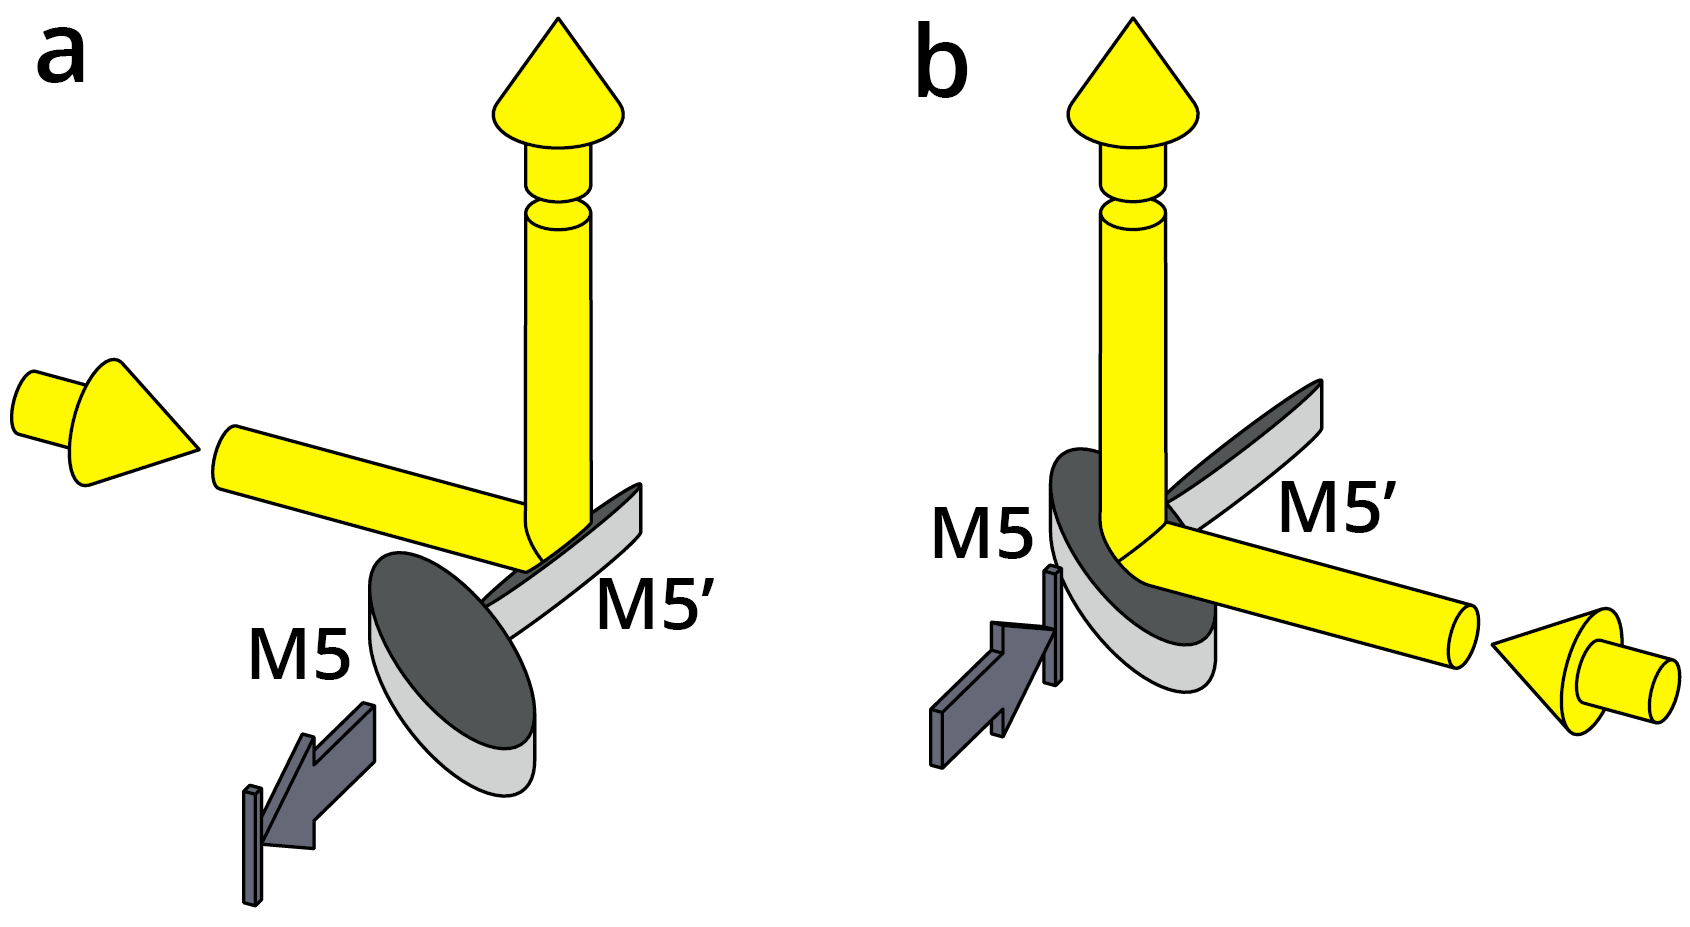
\includegraphics[width=0.8\textwidth]{SW/dualMirrorFigure}
        \bcaption[Detection branch switching unit]{To be able to image both views on the same camera, a moveable mirror unit is introduced. Depending on the imaging direction, the mirror block is either moved backward (\textbf{a}) or forward (\textbf{b}) to reflect the light up to the camera. Since the movement is parallel to the mirrors' surface, the image position on the sensor is not dependent on the exact position of the mirrors.}
        \label{fig:dualMirror}
      \end{figure}
        
      


     %##    ##       ####  ######   ##    ## 
    %# ##   ##        ##  ##    ##  ###   ## 
   %#   ##  ##        ##  ##        ####  ## 
  %#     ## ##        ##  ##   #### ## ## ## 
  %######## ##        ##  ##    ##  ##  #### 
  %#     ## ##        ##  ##    ##  ##   ### 
  %#     ## ######## ####  ######   ##    ## 
\section{Optical alignment}
  Precise alignment of the illumination and detection paths are crucial for high quality imaging, and has a pronounced  importance for high magnification and high resolution optical systems. The DualMouse SPIM contains two illumination and detection paths 
  Due to the symmetrical setup of the microscope, we will only describe the alignment of one side, as the same procedure is also applicable to the other side.

  \subsection{Alignment of illumination branches}

    The two illumination branches start with a common light source, a single mode fiber coupled to laser combiner, and they also share a galvanometric mirror that performs the beam scanning to generate the virtual light-sheet. Likewise shared is a scan lens focusing on the galvo mirror (GM), and the illumination splitter unit (PM, see Section \ref{sec:splitter}).

    Alignment for the illumination arms are done in three steps. First the laser beam is aligned on the first rail that holds the galvo, lens L1, and the splitter unit PM. This is performed by two kinematic mirrors placed between the fiber output and the galvo mirror (not shown on figure). Using these two mirrors it is possible to freely align the beam along all 4 degrees of freedom: translation in two orthogonal directions, and rotation around two orthogonal axes. Beam alignment on the rail is tested by two irises at the two ends of the rail, if the beam passes through both of them we consider it centered and straight on the optical axis.

    After the beam is aligned on the first rail, lens L1 and the splitter unit PM are placed in the measured positions to image the galvo mirror on mirror M1 using lenses L1 and L2. Correct positioning of the splitter unit along the rail is crucial, since this will affect the lateral position and tilt of the beam exiting the unit. To some extent, this can also be compensated by adjusting the two mirrors before the galvo mirror, but is avoided if possible as this will also displace the beam from the center of the galvo mirror.

    After rough alignment of the illumination arms, when the laser is already coupled in the objective, the fine adjustments are performed based on the image of the beam through the other objective. The beam is visualized by filling the chamber with a 0.1\% methylene blue solution. As this solution is fluorescent, and can be excited in a very large range, it is well suited to visualize the beam during adjustment.

    \paragraph{Adjusting beam position}
      Beam position can be adjusted by either translating the beam in a conjugated image plane (I'), or by rotating the beam in a conjugated back focal plane (BFP'). The setup was designed in a way, that BFP' coincides with mirror M1. This mirror is mounted in a gimbal mirror mount, allowing to rotate the mirror exactly around its center, which avoids unwanted translational movements, and results in pure rotation of the beam. Lens L3 is positioned exactly 1 focal length from the mirror, thus acting as a scan lens, and transforming the rotational movements to translation. This translation is further imaged and demagnified by the tube lens L4 and the objective O onto the sample.


    \paragraph{Adjusting beam tilt}
      Beam tilt can be adjusted by either rotating the beam in an intermediate image plane (I'), or translating it at the back focal plane (BFP). As mirror M2 is relatively far from the back focal plane, adjusting this will mostly result in translation that will rotate the beam. This movement, however will also introduce translations, and has to be compensated by adjusting mirror M1. The light-sheet, however needs to be tilted by \SI{30}{\degree} to coincide with the focal plane of the other objective, and this degree of adjustment is not possible with M2. In order to allow for a pure rotation of the light-sheet, we mounted the dichroic mirrors on a linear stage (OptoSigma, TSDH-251C). By translating the dichroic mirror, the illumination laser beam gets translated at the back focal plane, which will result in a pure rotational movement at the sample. Rough alignment of the light-sheet is performed by adjusting the dichroic position while inspecting the light-sheet through a glass window in the chamber. Precise alignment is then done based on the image of the beam visualized in a fluorescent medium.


    % \paragraph{Adjusting beam axial position.}


    \paragraph{Adjusting scanning plane angle}
      After the beam is properly aligned, i.e. it is in focus, and in the center of filed of view, it is still necessary to check if the scanning direction is parallel to the imaging plane. It is possible that the beam is in focus in the center position, but when moved up or down it drifts out of focus due to a tilted scanning angle. This tilt can be compensated by mirror M1, that is placed at the conjugated back focal plane BFP'. Between lenses L3 and L4 a magnified version of the light-sheet will be visible, and the tilt can be checked by placing an alignment target in the optical path while scanning the beam. By tilting mirror M1 up or down, the scanning pattern not only moves up or down, but is also rotated if the mirror surface is not exactly vertical. Since M1 and GM are in conjugated planes, the tilt and offset can be performed independently. The tilt is first fixed by M1 while inspecting the target, and the beam is re-centered by changing the offset on the galvo mirror. Moving the galvo mirror will not introduce tilt, since in this case rotation axis is perpendicular to the reflection plane.




  \subsection{Alignment of detection branches}
    Since the detection path is equivalent to a wide-field detection scheme, its alignment is much simpler than that of the illumination branches. The only difference is the detection branch merging unit (see \autoref{sec:dualMirror}.) that features two moving mirrors. This, however doesn't effect the alignment procedure, since the movement direction is parallel to both mirror's surface, meaning that the exact position of the mirrors will not affect the image quality, as long as the mirrors are not clipping the image itself. Stability test were performed to confirm the consistent switching performance of the mirror unit before the final alignment took place (see Sec. \ref{sec:mirrorStability}).

    % TODO: complete paragraph
    The final alignment procedure 

    \paragraph{Positioning the tube lens}
      The position of the tube lens determines the focal plane the is being imaged on the camera sensor. Ideally, the tube lens' distance from the camera sensor is exactly the tube lens focal length, which will ensure the best imaging performance. If the tube lens distance is not correct, the focal plane will be slightly shifted in the axial direction. Although small shifts will not necessarily have detrimental effect on the image quality, because the light sheet can also be shifted accordingly. Because of the shifted focal and image planes, however, the magnification of the system will be affected, and will change depending on the amount of defocus. For this reason we aim for positioning the tube lens as close to the theoretical position as possible.

      Our tube lens is a compound, achromatic lens with a center thickness of \SI{12.5}{mm}, and edge thickness of \SI{11.3}{mm}. Its effective focal length is \SI{400}{mm} which will produce a 50x magnified image. Back focal length is \SI{394.33}{mm} which we measured form the camera chip, and the lens was positioned at this theoretically optimal position.

    \paragraph{Adjusting correction collar}
      The Nikon 25x objectives used for this setup have a built in correction ring that can be used to correct spherical aberrations resulting from refractive index differences when imaging samples behind a coverslip. This can be also effectively used to correct for any spherical aberrations occurring from imaging through the FEP foil. Although these aberrations are expected to be extremely low, due to the relatively thin, \SI{50}{\micro m} foil thickness, and the close matching of refractive index ($n_{FEP} = 1.344$, $n_{H_2O}=1.333$), for optimal, aberration free image quality it can't be neglected.

      The correction collars are adjusted by inspecting a gel suspended fluorescent bead specimen with the microscope, where the beads can act as a reporter of the point spread function of the microscope. The alignment can be performed ``live" by inspecting the bead image quality for any aberrations. By gradually changing the correction collar, the ring are minimized on out of focus beads, and the peak intensity is maximized for in focus beads. By moving the correction ring, the focal plane is also slightly shifted, which has to be compensated by shifting the light-sheet correspondingly to coincide with the correct imaging plane.

    \paragraph{Adjusting field of view}
      To allow for proper sampling of the image, we use 50x magnification, which, combined with the \SI{6.5}{\micro m} pixel pitch of our sCMOS camera will result in a \SI{0.13}{\micro m} pixel size. The full field of view with this magnification is $2048 \times 0.13 = \SI{266.24}{\micro m}$. The full field of view the objective provide, are larger than this, at \SI{800}{\micro m}. To ensure the best image quality, we align the center of the objective field of view on the camera sensor, since this region has the best optical properties in term of numerical aperture, aberration correction and field flatness.

      Field of view alignment can be performed using mirror M4 just before the detection merging unit. To identify the center region of the field of view, diffuse white light is used to illuminate the entire sample chamber, and is imaged on the camera. Then, mirror M4 is adjusted until the top edge of the field of view becomes visible, \textit{i.e.} where the illumination from the chamber is clipped. This will have a circular shape. Then, adjusting the mirror in the orthogonal direction, the left-right position of the field of view can be adjusted, by centering the visible arc on the camera sensor.

      After the horizontal direction is centered, vertical centering is performed. This, however can't be centered the same way as the horizontal direction, since for that we would have to misalign the already aligned horizontal position. To determine the center, we move the field of view from the topmost position to the bottom. During this process the number of  turns of the adjustment screw is counted (this can be done accurately by using a hex key). After reaching the far end of the field of view, the mirror movement is reversed, and the screw is turned halfway to reach the middle.







\section{Control unit}

  The microscope's control and automation is performed by an in-house designed modular microscope control system developed in LabVIEW \cite{balazs_development_2013}. The core of the system is a National Instruments cRIO-9068 embedded system that features and ARM Cortex A9 processor, and a Xilinx Zynq 7020 FPGA.
  Having both chips in the same device is a great advantage, since the main processor can be used to run most of the microscope control software, while the FPGA can be used to generate the necessary output signals in real time and with high precision.
  
  The embedded system is complemented by a high performance workstation that is used to display the user interface of the microscope, and to record the images of the high-speed scientific complementary metal–oxide–semiconductor (sCMOS) camera. 

  \subsection{Hardware}
    Various components need to be synchronized with high precision to operate the microscope: a laser combiner to illuminate the sample; a galvo scanner to generate the light-sheet; stages to move the samples; filter wheel to select the imaging wavelengths; and a camera to detect the fluorescence.    
    % For more details on the exact models, see Appendix \ref{sec:BOM}.
    For high speed image acquisition, all of these devices have to be precisely synchronized in the millisecond range, and some even in the microsecond range.
    Although they require different signals to control them, we can split them into three main categories:

    \begin{center}
      \begin{tabular}{lll}
        \textbf{digital input} & \textbf{analog input}   & \textbf{serial communication} \\ \hline
        camera exposure    & galvo position & filter wheel         \\
        laser on/off (\texttimes 3) & laser intensity (\texttimes 3) & stages (\texttimes 2)
      \end{tabular}
    \end{center}

    All devices are connected to the NI cRIO 9068 embedded system, either to the built in RS232 serial port, or to the digital and analog outputs implemented by C-series expansion modules (NI 9401, NI 9263, NI 9264). The workstation with the user interface is communicating with the embedded system through the network. The only device with a connection to both systems is the camera: the embedded system triggers the image acquisition, while the images are piped to the workstation through a dual CameraLink interface, capable of a sustained \SI{800}{MB/s} data transfer rate (\autoref{fig:HW}).

    \begin{figure}
      \centering
      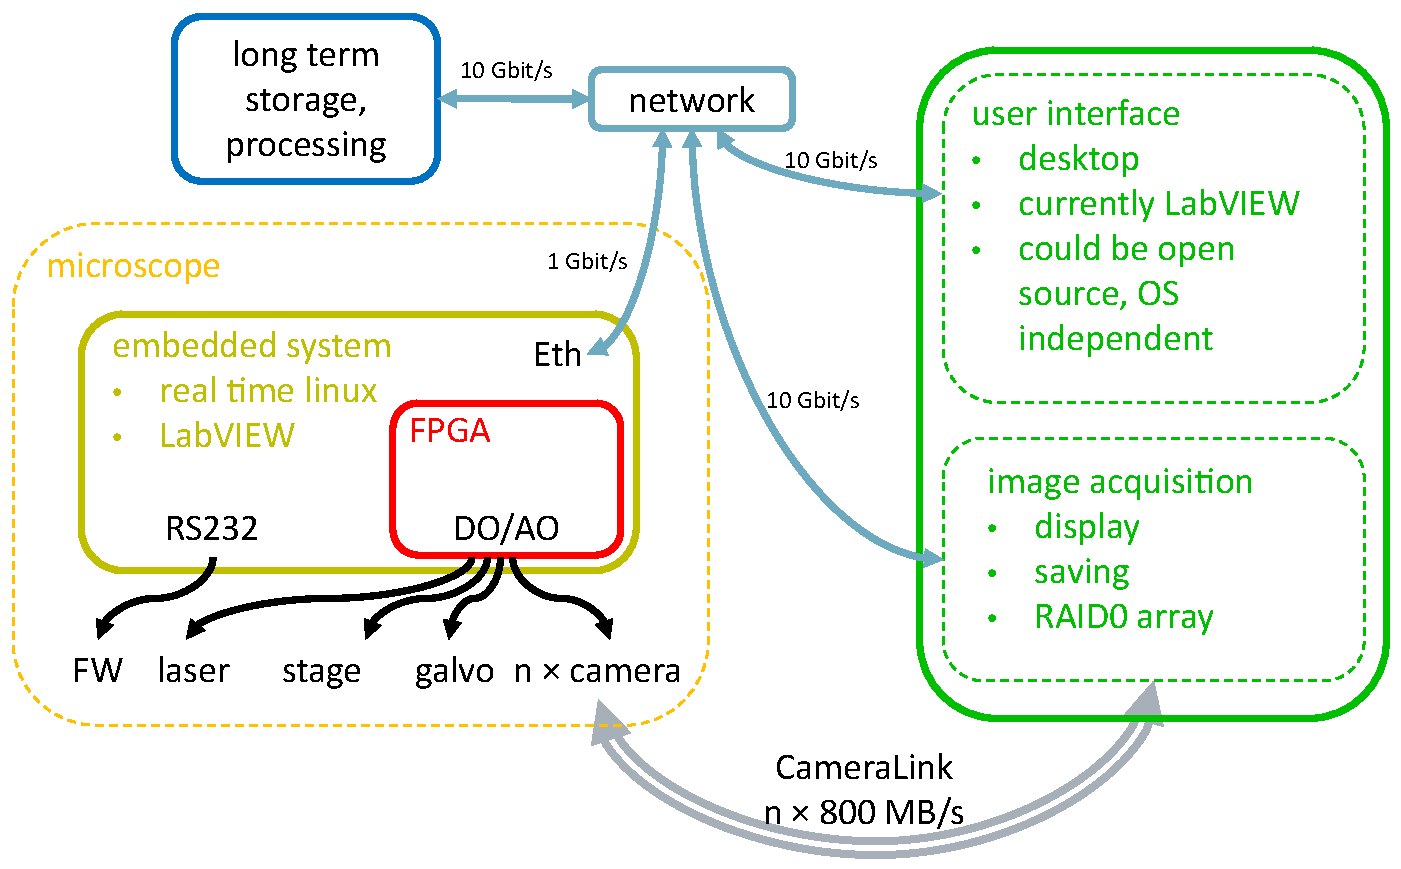
\includegraphics[width=0.9\textwidth]{HW}
      \bcaption[Microscope control hardware and software architecture]{The embedded system responsible for the hardware control and the workstation are communicating through the network using the WebSocket protocol. The electronic devices of the microscope are either controlled through digital/analog signals, or through serial communication. The camera }
      \label{fig:HW}
    \end{figure}
  
  \subsection{Software}
    \label{sec:software}

    \begin{figure}
      \centering
      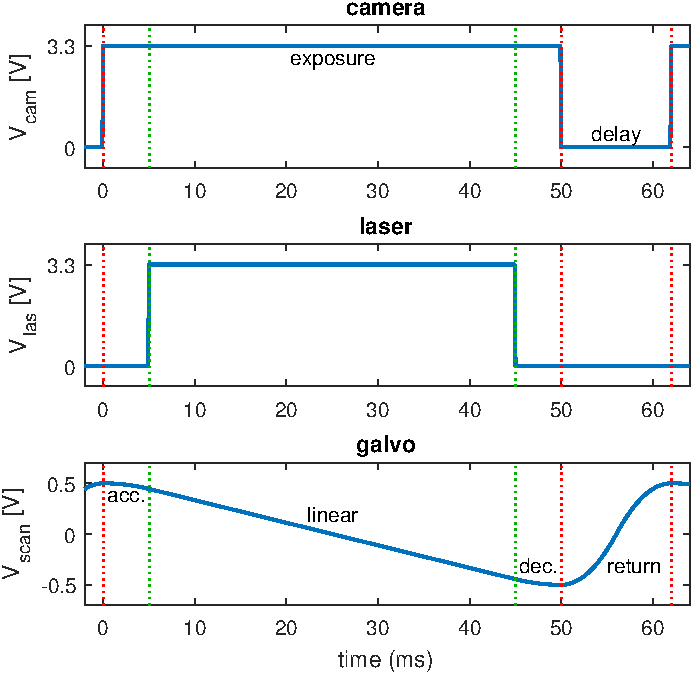
\includegraphics[width = 0.6\textwidth]{fpgaTraces}
      \bcaption[Digital and analog control signals]{Example traces for recording a single plane with \SI{50}{ms} exposure time and \SI{12}{ms} delay. During the exposure of the camera the galvo has 3 sections: acceleration (acc.), linear, and deceleration (dec.). The laser line is synchronized with the galvo linear section to ensure even illumination. }
      \label{fig:traces}
    \end{figure}

    Being able to precisely control all of the instruments not only relies on the selected hardware, but just as much on the software. Our custom software is developed in LabVIEW, using an object oriented approach with the Actor Framework. The embedded system is responsible for the low level hardware control, for keeping track of the state of all devices, saving the user configurations, and automating and scheduling the experiments. It also offers a Javascript Object Notation (JSON) based application programming interface (API) through WebSocket communication. This is mainly used to communicate with the user interface, however it also offers the possibility of automated control by an external software.

    \subsubsection{FPGA software}
      The on-board FPGA is responsible for generating the digital and analog output signals based on the microscope settings (\autoref{fig:traces}). To avoid having to calculate all the traces for a whole stack, the main software only calculates a few key parameters of the traces that are necessary to completely describe them. The FPGA then calculates the output signals in real time, and outputs them with microsecond precision.

      To describe the traces, we define them as a concatenation of \textit{sections}. Each section has 3 or 5 parameters, depending if their type is digital or analog. Both types have 3 common properties: \texttt{value}, \texttt{length}, and \texttt{type}. The analog sections additionally contain a \texttt{dValue} and a \texttt{ddValue} element describing the velocity and the acceleration of the signal. This allows us to generate piecewise functions made of second order polynomials.

      The \texttt{type} element contains information on which value should be updated for the current section. Setting the lowest bit high will update the \texttt{value}, setting the second bit high will update the \texttt{dValue}, and setting the third bit high will update the \texttt{ddValue}. This feature allows to define smooth transitions between the sections, and also to define more complex signals, as long as they are periodic in the second derivative.


    %#######  ########  ######  ##     ## ##       ########  ######  
    %#     ## ##       ##    ## ##     ## ##          ##    ##    ## 
    %#     ## ##       ##       ##     ## ##          ##    ##       
    %#######  ######    ######  ##     ## ##          ##     ######  
    %#   ##   ##             ## ##     ## ##          ##          ## 
    %#    ##  ##       ##    ## ##     ## ##          ##    ##    ## 
    %#     ## ########  ######   #######  ########    ##     ######  
\section{Results}
  \begin{figure}
    \begin{subfigure}[t]{0.5\textwidth}
      \centering
      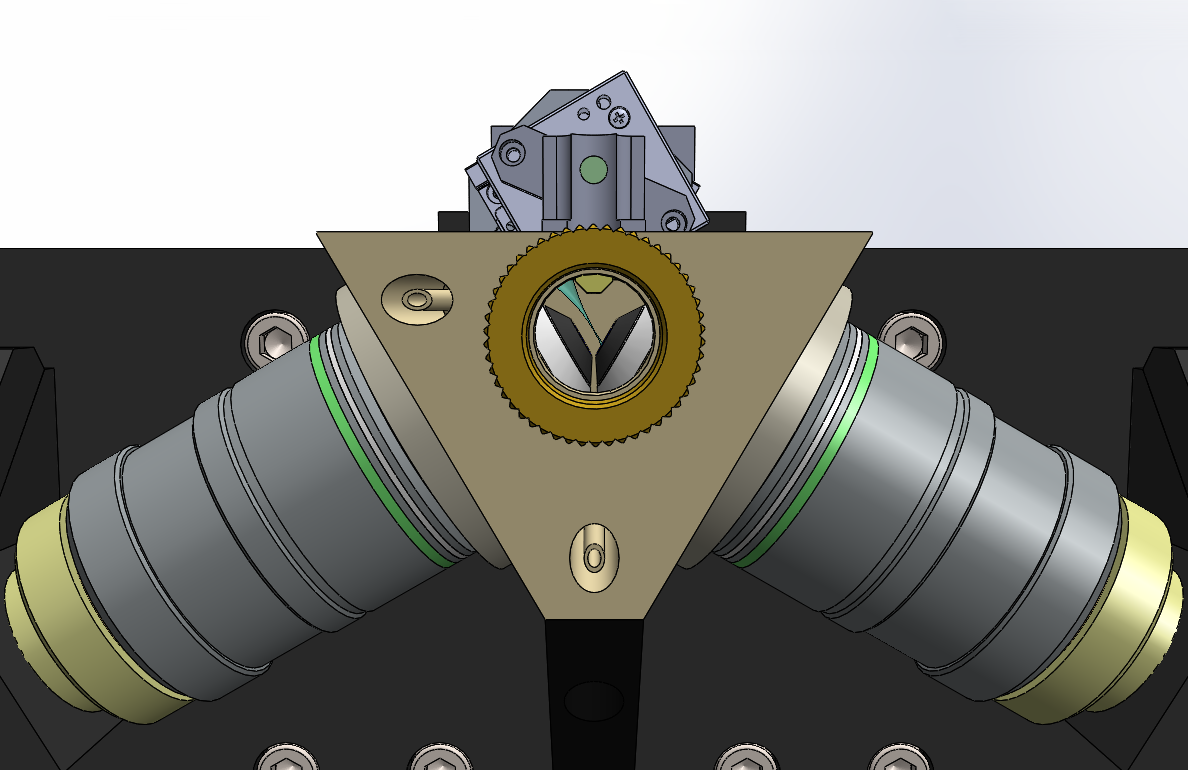
\includegraphics[width=\textwidth]{photos/front_solidworks_overlay}
      \caption{Front view of the SolidWorks design.}
    \end{subfigure}
    \begin{subfigure}[t]{0.5\textwidth}
      \centering
      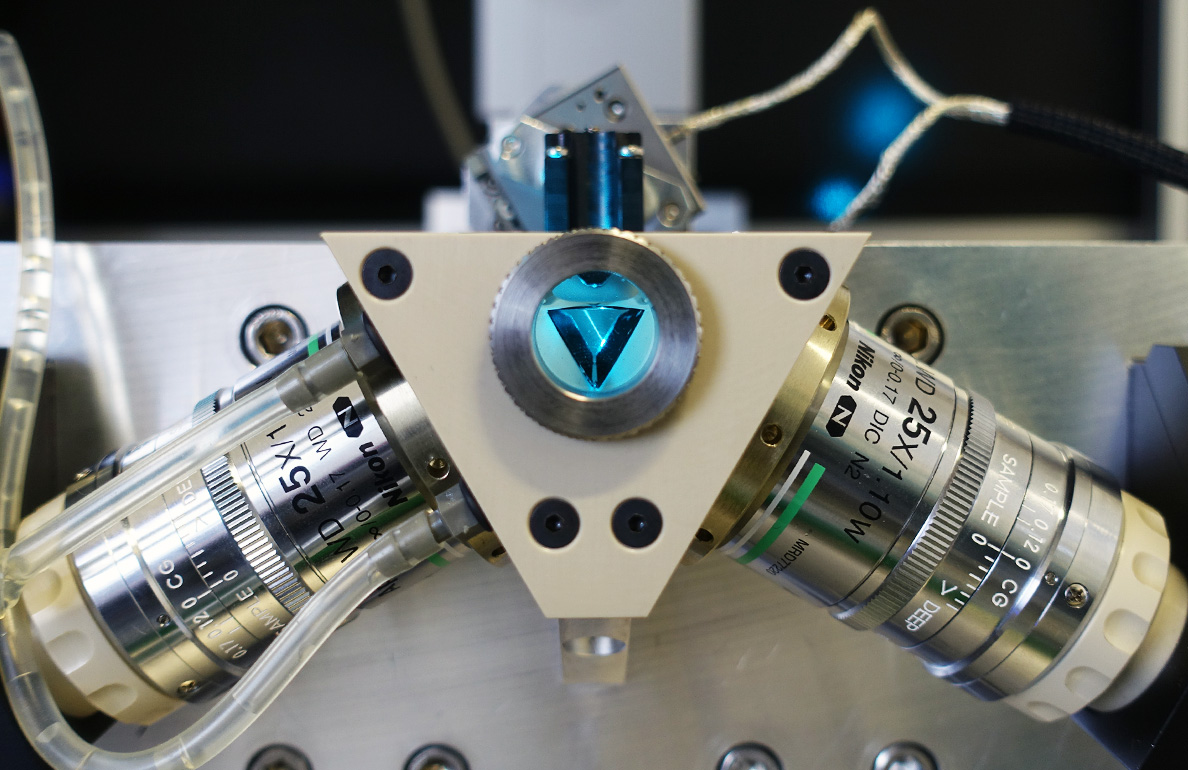
\includegraphics[width=\textwidth]{photos/front_photo_overlay.jpg}
      \caption{Front view of the microscope.}
    \end{subfigure}
    \\
    \begin{subfigure}[t]{1\textwidth}
      \centering
      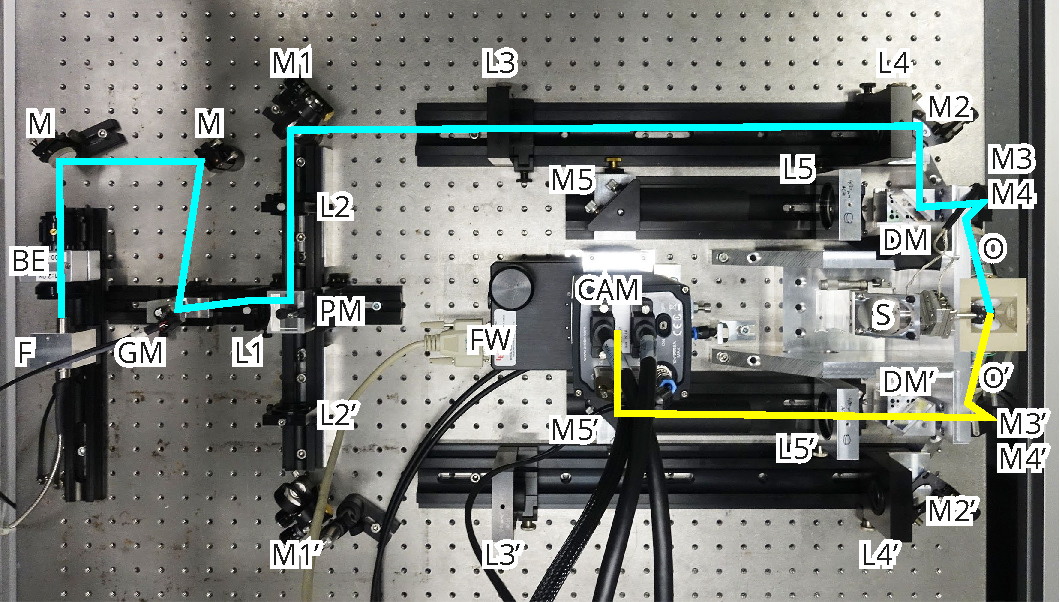
\includegraphics[width=\textwidth]{photos/top+light}
      \caption{Top view of the microscope.}
    \end{subfigure}
    \bcaption[Completed DualMouse-SPIM]{The excitation and emission light paths are depicted with blue and yellow lines respectively. Component numbering corresponds to \autoref{fig:fullSchematics}. Detection branch merging unit, and mirrors M6 and M6' are underneath the camera and filter wheel. BE -- beam expander, CAM -- camera, DM -- dichroic mirror, F -- fiber, FW -- filter wheel, L -- lens, M -- mirror, O -- objective, PM -- prism mirror, S -- stage}
    \label{fig:frontView}
  \end{figure}

  % Resolution for Lattice light-sheet \cite{chen_lattice_2014}: \SI{230}{nm} in x and \SI{370}{nm} in z
  % \cite{chhetri_whole-animal_2015}

  After the design phase, all custom parts were manufactured by the EMBL mechanical workshop, and microscope was assembled on a NewPort "!!!type!!!" optical table (Fig. \ref{fig:frontView}). The microscope was equipped with an Andor Zyla 4.2 sCMOS camera, that offers a large field of view of 2048\texttimes 2048 pixels with a pixel pitch of \SI{6.5}{\micro m}. It offers a high dynamic range of 1:30,000, and high frame rate at 100 frames per second (fps), while readout noise is minimal (0.9 e$^-$).
  
  To evaluate the performance of the microscope, we conducted various measurements, concerning the stability and the resolution of the system. The methods and results of these measurements will be presented in this section.


  \subsection{Stability of view switcher unit}
    \label{sec:mirrorStability}

    \begin{figure}
      \centering
      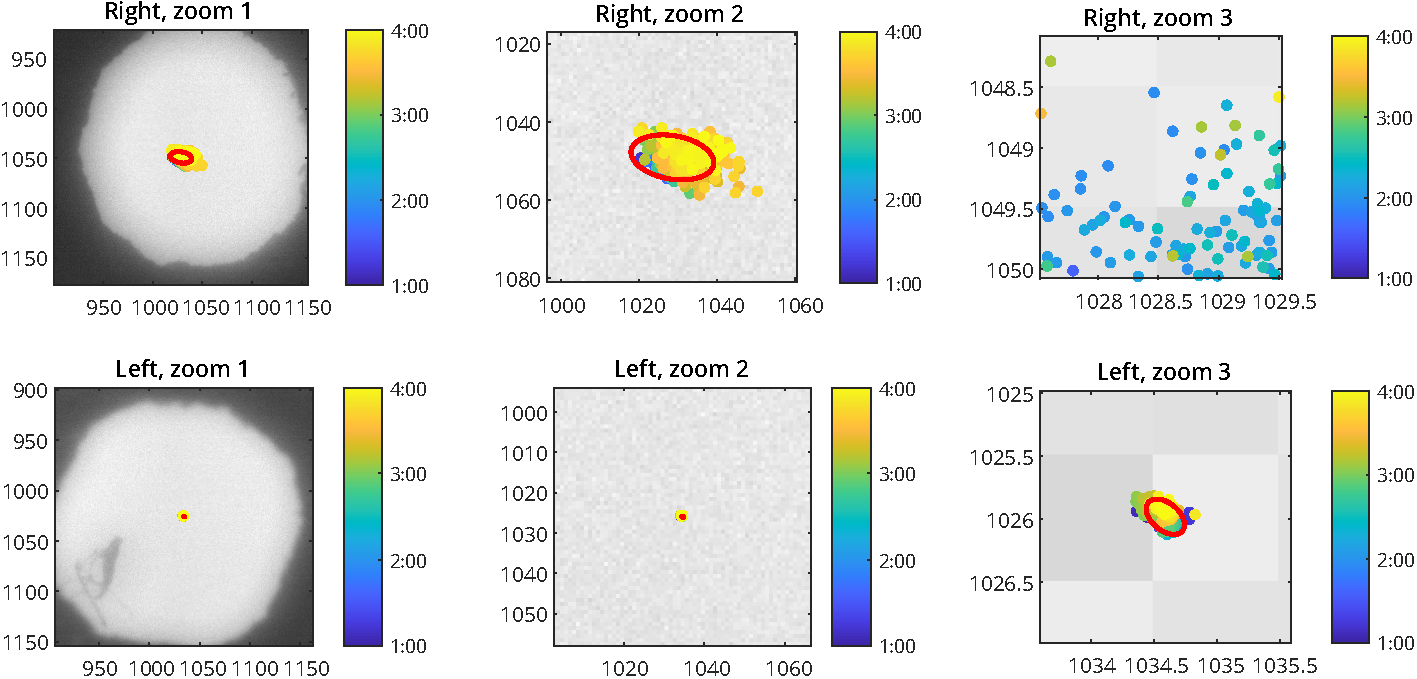
\includegraphics[width=\textwidth]{trackCenter}
      \bcaption[Stability measurements of view switcher unit] {A closed aperture was imaged on the camera from both views, every \SI{10}{s}, for \SI{4}{h}. The dots represent the center of each frame, color coded with the time. The red ellipse represents the 95\% confidence interval of the measured positions based on principal component analysis. Standard deviations for right view: $\sigma_1 = \SI{4.37}{px}$, $\sigma_2 = \SI{2.26}{px}$; for left view: $\sigma_1 = \SI{0.07}{px}$, $\sigma_2 = \SI{0.04}{px}$.}
      \label{fig:stability}
    \end{figure}

    As the view switcher unit is a custom designed solution for this microscope, it is necessary to evaluate the effect of the switching on the field of view. Because this is a moving unit, many mechanical imprecisions can introduce a drift in the final image. 

    To assess the reproducibility in the movement of the detection branch switching unit, a long term stability test was conducted. To exclude all other factors (such as sample drift), we imaged the opening of two closed irises that were mounted on the detection optical rail. Image formation was done by two achromatic lenses ($f=\SI{75}{mm}$) positioned directly after mirrors M5 and M5'.
    
    The apertures were imaged from both views every 10 seconds, for \SI{4}{h}, for a total of 1440 images per view, and 2880 switches. The center of the aperture was segmented on all images using Matlab, and tracked to assess any drift occurring during the \SI{4}{h} time lapse (\autoref{fig:stability}). To visualize the uncertainty of the aperture's position, we performed principal component analysis (PCA) on the positions and visualized the results by plotting the 95\% confidence ellipse on the images. Although the right view had a significant spread with a standard deviation of \SI{4.37}{px} and \SI{2.26}px along the long ans short axes respectively, the left view was extremely stable, and the standard deviation was only \SI{0.07}{px} and \SI{0.04}{px} for the long and short axes respectively. This result implies that there is no conceptual limitation in reaching sub-pixel reproducibility with the view switching unit, although some optimization is still needed for the right view to reach the same stability as the left view. 

    

  \subsection{Characterizing the illumination profile}

    \begin{figure}[hbt]
      \centering
      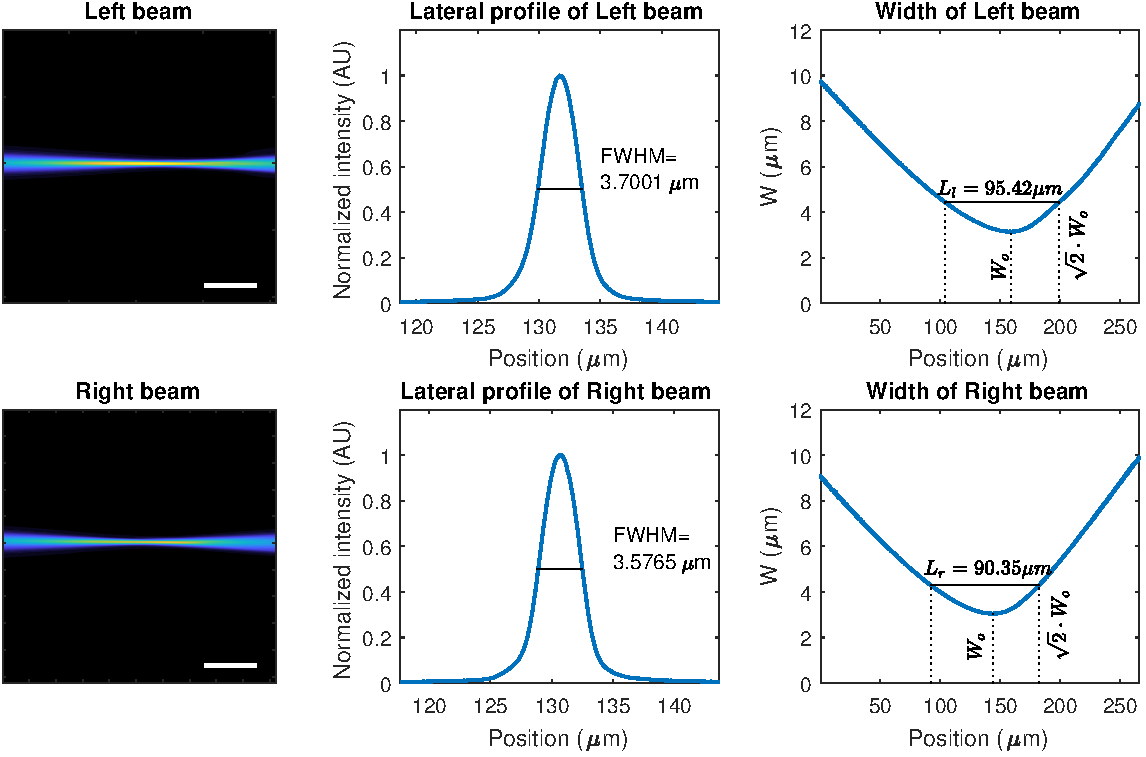
\includegraphics[width=\textwidth]{beamPlots.pdf}
      \bcaption[Illumination beam profile]{Average of 500 stationary beam images for both left (top left) and right objectives (bottom left). Beam intensity profile along the waist of each beam is plotted in the center column. The right column shows the beam width profile of each beam ($1/e^2$).}
      \label{fig:beamProfiles}
    \end{figure}

    Since a Gaussian beam is used for illumination, its intensity profile is dependent of the axial position (\autoref{eq:gaussian}). Although the total intensity at any cross section of the beam is constant, because of the divergent properties, the peak intensity varies. To assess any non-uniformities in the illumination pattern, we measured the illumination beam intensity for each view.

    To visualize the beam, the chamber was filled with a fluorescent solution (0.1 \% methylene blue in distilled water). In order to increase the signal to noise ratio of these images, a long exposure time of \SI{200}{ms} was used, and 500 images of each beam was averaged, and the background subtracted (\autoref{fig:beamProfiles}). Background images were acquired by repeating the image acquisition with the laser turned off, and averaging the recorder dark images.

    To determine the beam waist position, we measured the beam thickness (FWHM) for each column of the averaged images, and located the position of the minimal width. The beam width at the waist position for the left view was   \SI{3.70}{\micro m}, and for the right view it was \SI{3.58}{\micro m} (\autoref{fig:beamProfiles}). We also measured the usable length of the beams (\ref{sec:dimensions}). The distance between the points where the beam has expanded by a factor of $\sqrt2$ relative to the waist is \SI{95.42}{\micro m} for the left view, and \SI{90.35}{\micro m} for the right view. This corresponds well to the original requirement of a minimal field of view of \SI{100}{\micro m}. Depending on the sample however, the practical field of view can be larger than this, as the camera sensor allows for a field of view of \SI{266}{\micro m}.  

    


  


  \subsection{Resolution and point spread function measurement}

    In order to establish an ideal, reference PSF, we simulated the theoretical PSF of the microscope with the Gibson-Lanni model \cite{gibson_experimental_1992}, using the MicroscPSF Matlab implementation \cite{li_fast_2017}. The advantage of this model is that is accounts for any differences between the experimental conditions and the design parameters of the objective, and thus it can simulate any possible aberrations that should arise. The adjustable parameters are the thicknesses ($t$) and refractive indices ($n$) of the immersion medium ($i$), coverslip ($g$), and sample ($s$). To simulate the reference PSF, we accounted for the slight mismatch in refractive index between the FEP foil ($n_g = 1.344$) and water ($n_i = 1.33$). The working distance of the objective is \SI{2}{mm}, while the thickness of the foil is \SI{50}{\micro m}. 

    \begin{figure}
      \centering
      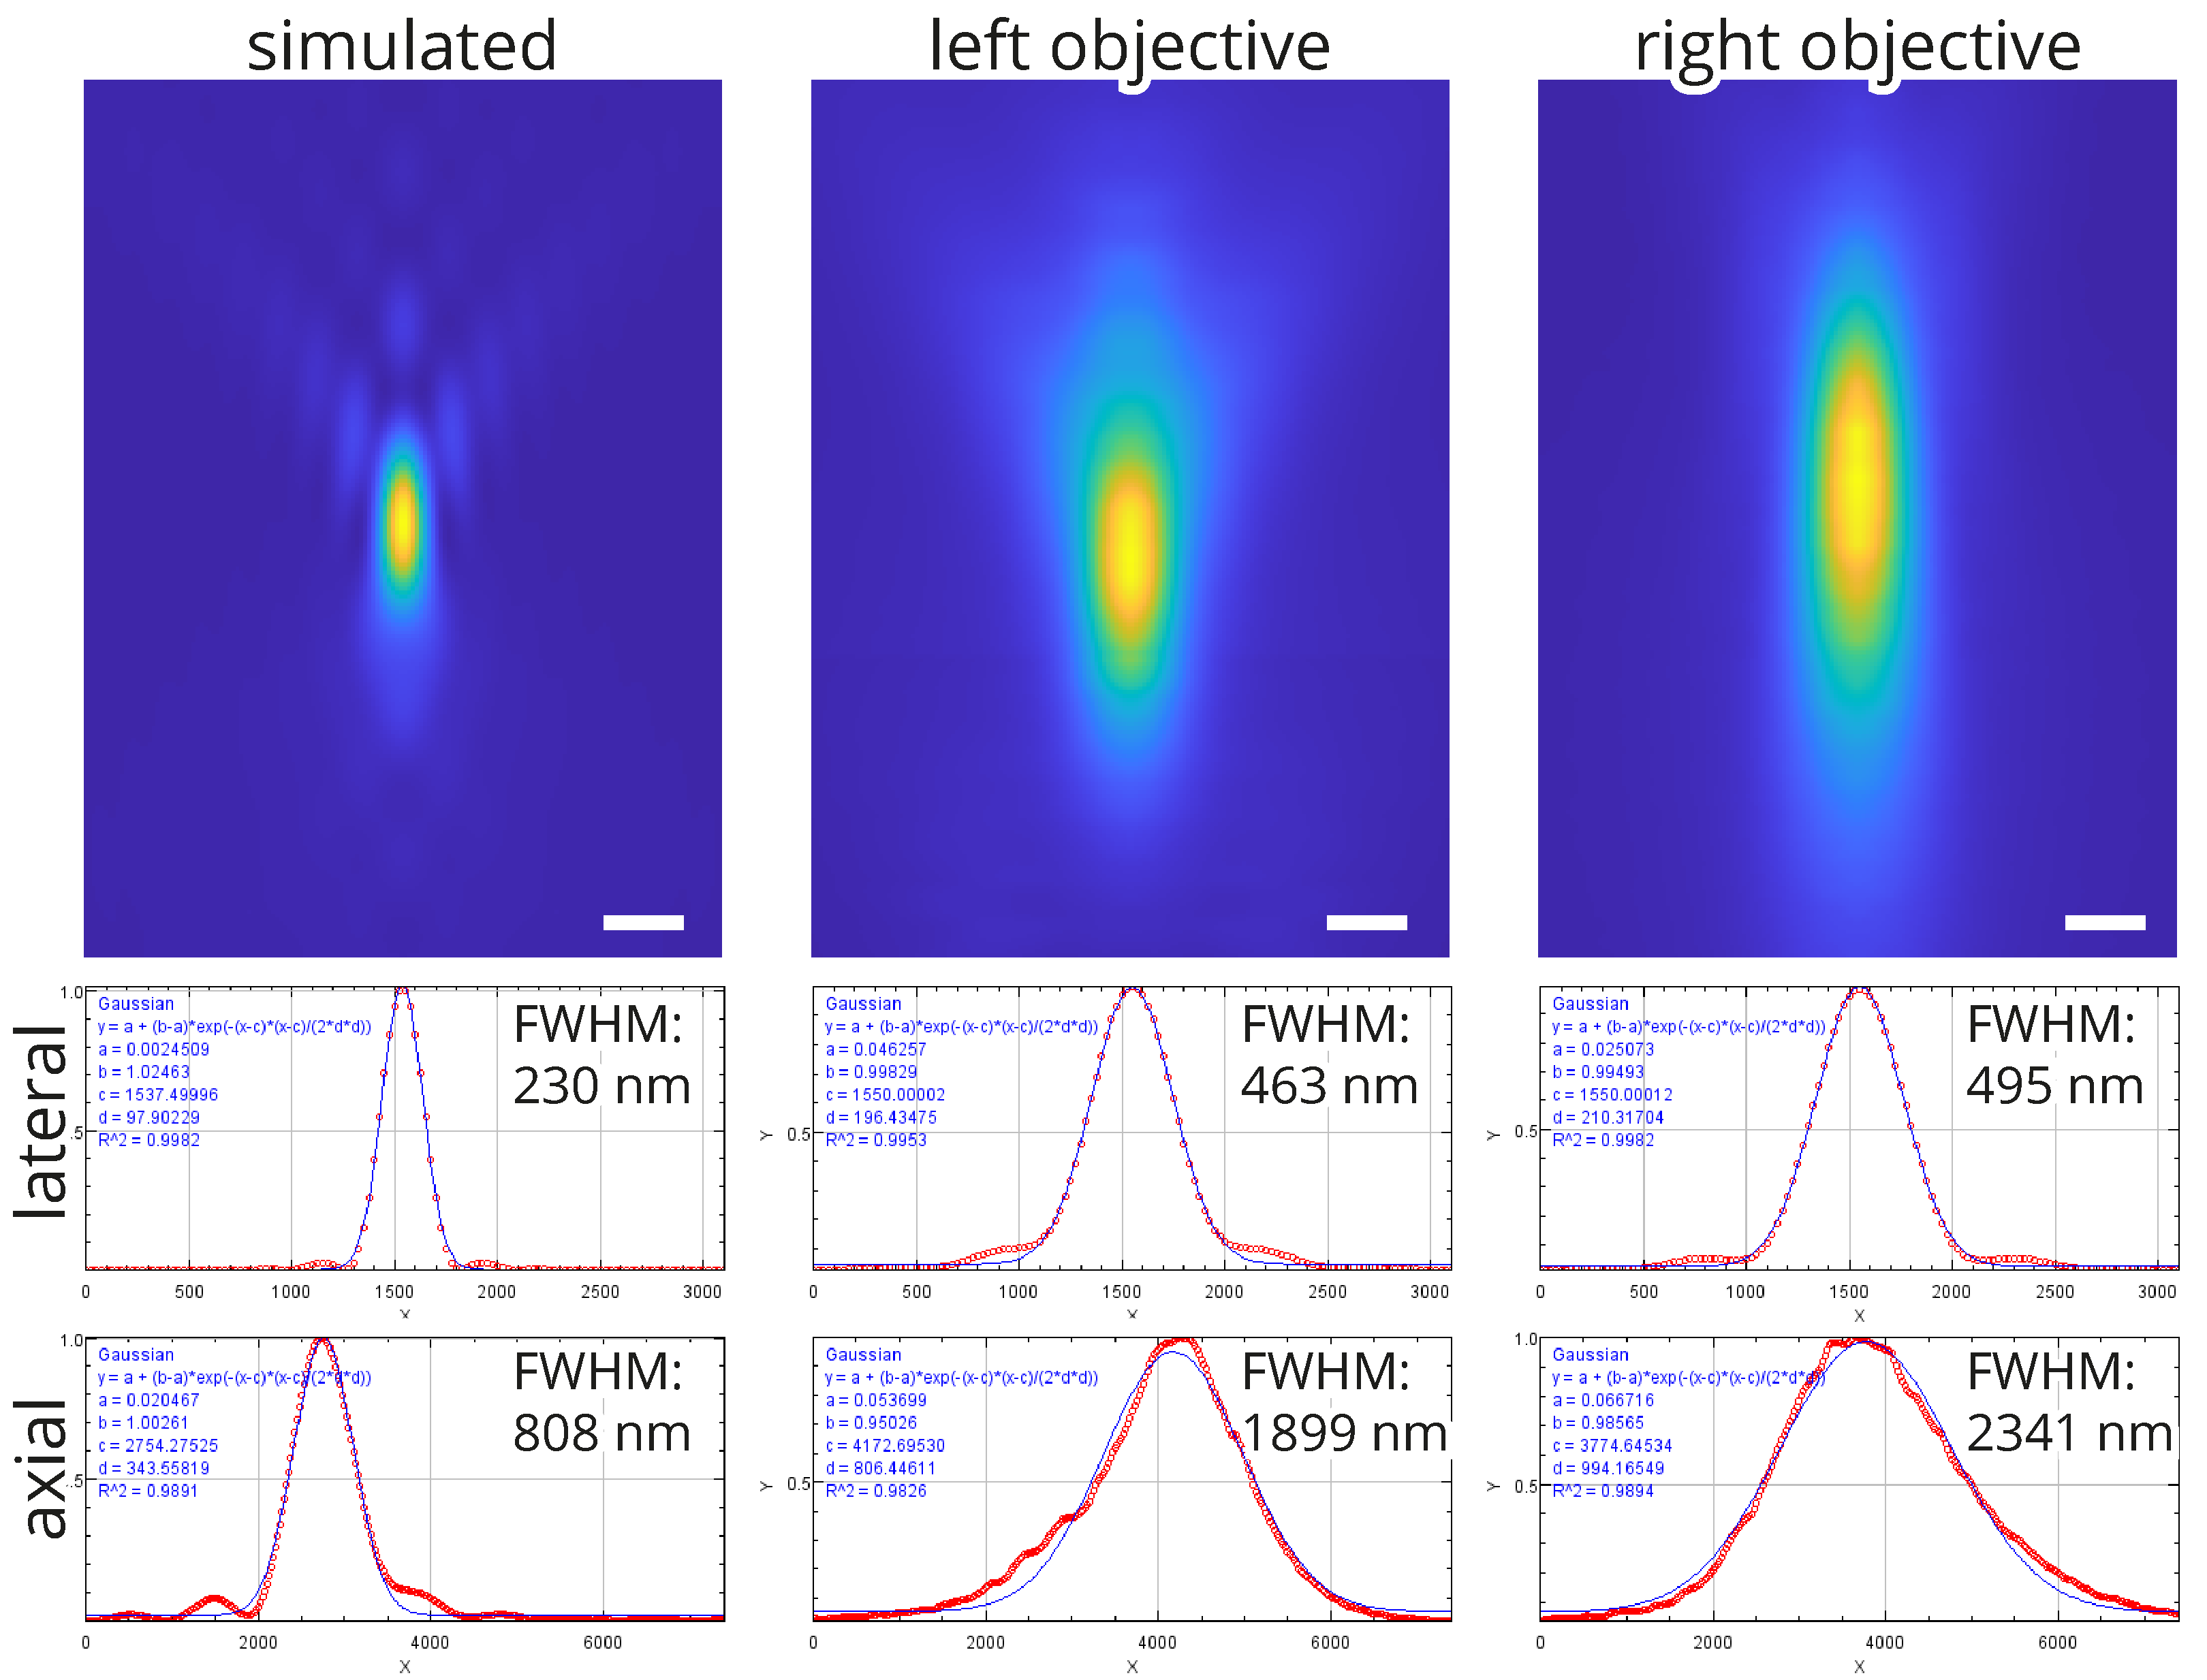
\includegraphics[width=\textwidth]{PSF}
      \bcaption[Simulated and measured PSF of Dual Mouse-SPIM]{Top row: axial sections of simulated and measured point spread functions. Middle row: lateral intensity profile and Gaussian fit. Bottom row: Axial intensity profile and Gaussian fit. Simulations were performed based on the Gibson-Lanni model. Immersion medium  and sample refractive index: 1.330, coverslip (FEP foil) refractive index: 1.344, coverslip distance: \SI{1900}{\micro m}, coverslip thickness: \SI{50}{\micro m}. Excitation wavelength: $\lambda_{ex} = \SI{561}{nm}$. Emission wavelength: $\lambda_{em} = \SI{600}{nm}$. Scale bar: \SI{1}{\micro m}.}
      \label{fig:measuredPSF}
    \end{figure}

    It is apparent from the simulations that even though the FEP refractive index is almost identical to the refractive index of water, a slight spherical aberration is still present even for the ideal case (\autoref{fig:measuredPSF}, left). The resolution measured as the FWHM of the intensity profile through the lateral and axial cross sections is \SI{271}{nm} and \SI{866}{nm} respectively. FWHM was measured in Fiji by fitting a Gaussian curve, and multiplying the standard deviation of the resulting fit by $2 \sqrt{2 \ln 2}$.

    % \subsubsection{Methods}
    To experimentally measure the resolution of the microscope and characterize its optical performance, we measured the point spread function using fluorescently labeled beads suspended in 0.8\% GelRite (\autoref{sec:methods2}). The gel was loaded in glass capillaries  and allowed to cool. After the gel solidified, a $\sim$\SI{1}{mm} piece was cut off and placed in the microscope sample holder. The beads were imaged from both views using the \SI{561}{nm} laser line with the 561 long-pass filter (Semrock, BLP02-561R-25).

    From both views 12 beads were averaged using Fiji \cite{schindelin_fiji:_2012} and the 3D PSF estimator of the MOSAIC suite \cite{cardinale_imagej_2010}. In order to acquire a more accurate PSF, the averaged bead images were deconvolved with the ideal image of the bead (uniform sphere width a diameter of \SI{500}{nm}) using the DeconvolutionLab2 Fiji plugin \cite{sage_deconvolutionlab2:_2017}. The results of the deconvolution are shown on \autoref{fig:measuredPSF}. Similarly to the simulation, we measured the axial and lateral resolutions on the experimental PSFs. For the left view, the measured resolutions were \SI{386}{nm} in the lateral direction, and \SI{1350}{nm} in the axial direction. For the right view the lateral resolution was \SI{326}{nm}, and the axial was \SI{1297}{nm}.

    \begin{figure}
      \centering
      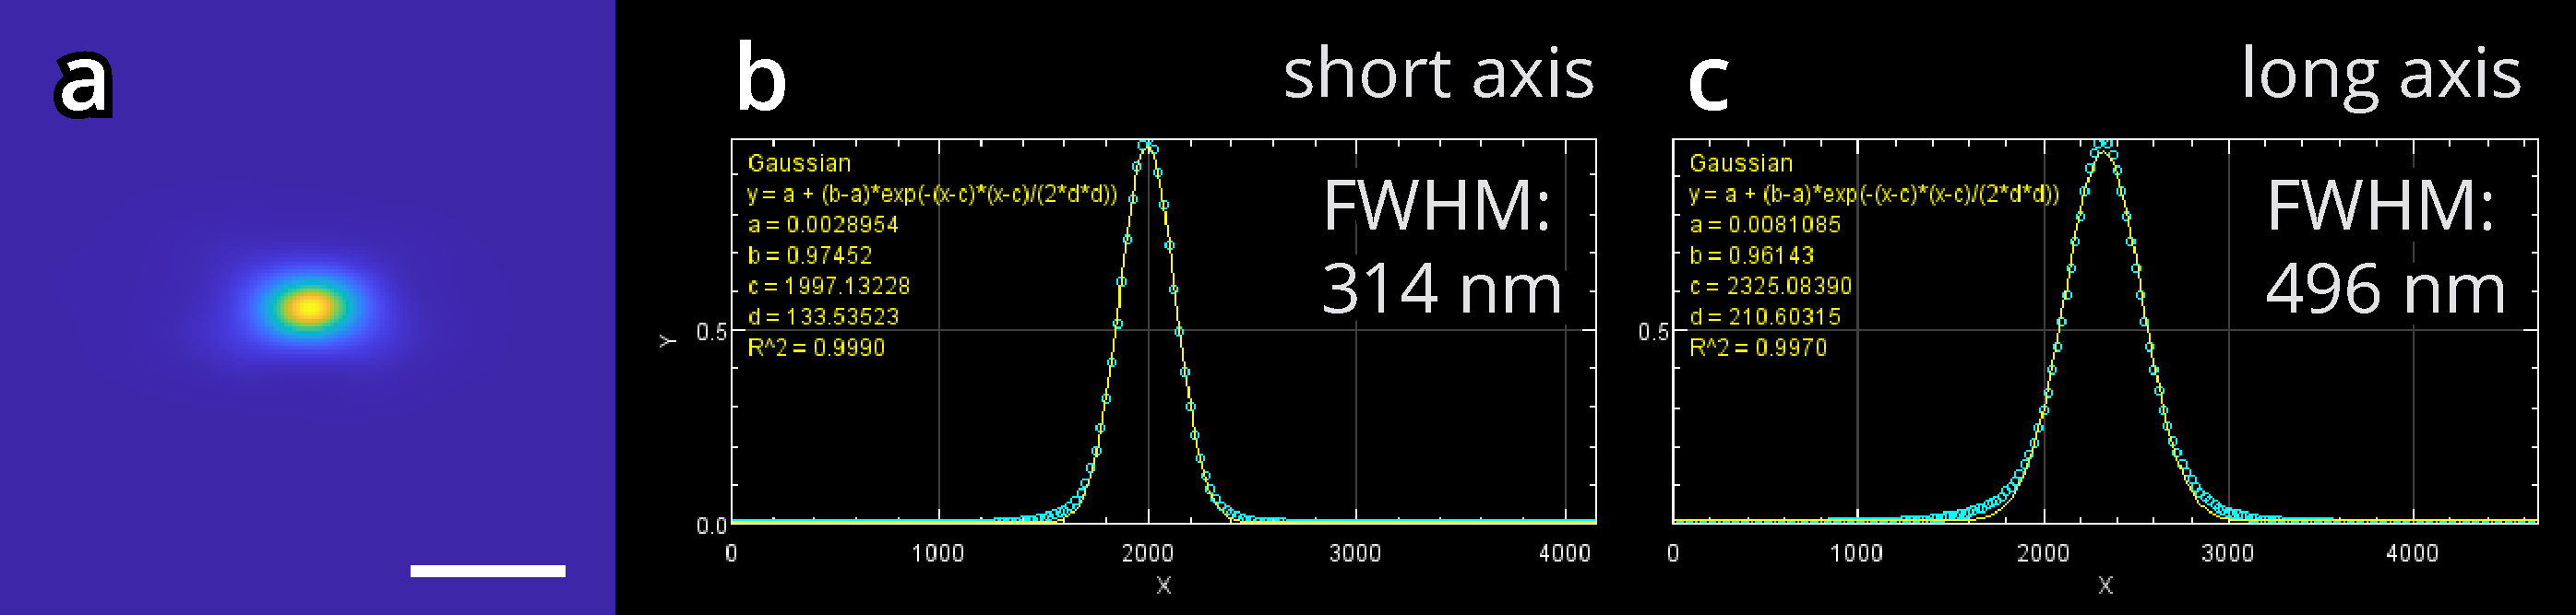
\includegraphics[width=0.9\textwidth]{beads/fusedPSF}
      \bcaption[Combined PSF of 2 views]{(\textbf{a}) The measured PSFs (\autoref{fig:measuredPSF}) were rotated to their corresponding orientations and multiplied. (\textbf{b}) Gaussian fit along the short axis of the combined PSF; FWHM=\SI{314}{nm}. (\textbf{c}) Gaussian fit along the long axis of the combined PSF; FWHM=\SI{496}{nm}.}
      \label{fig:fusedPSF}
    \end{figure}
    
    To estimate the achievable multi-view resolution of the system, we combined the two measured PSFs. First, the PSFs were rotated by $\pm \SI{60}{\degree}$ to correspond to the objective orientations. The PSF images were then normalized by scaling the maximum to 1, and the two rotated and normalized PSFs were multiplied (\autoref{fig:fusedPSF}). Resolution of the combined PSF is much improved in all directions: along its shortest axis the FWHM is \SI{314}{nm}, and along the longest axis the FWHM is \SI{496}{nm} (\autoref{fig:fusedPSF}). Both are better than the corresponding resolutions for a single view, especially along the long axis, where the resolution is 2.67 times better. This is almost perfectly matching the theoretically expected increase in the axial direction (compare with \autoref{sec:120concept}).


  \subsection{Resolution inside a \textit{Drosphila melanogaster} embryo}

    Apart from measuring the point spread function and resolution in an ideal bead sample, we also wanted to know the resolution inside a biological sample, as the tissues usually introduce some aberrations to the light path. Although these aberrations highly depend on the sample, as a worst case scenario, we measured the point spread function inside a \textit{Drosophila melanogater} embryo. As this specimen is highly opaque and scattering, it gives a good estimate for the upper bound of the resolution.

    Instead of the fluorescent beads, we imaged a \textit{Drosophila} embryo expressing H2A-mCherry marking the nuclei, and ASL-YFP marking the centrosomes (\autoref{fig:drosoEmbryo}a, and \autoref{sec:methods2}). As the centrosomal protein ASL is diffraction limited in size \cite{gonczy_towards_2012}, its image gives a good estimate for the point spread function inside the specimen.

    Similarly to the bead recordings, 15 centriole images were averaged with the 3D PSF tool of the MOSAIC plugin in Fiji (\autoref{fig:drosoEmbryo}c). On the averaged image we measured the resolution by fitting a Gaussian function on the lateral and axial intensity profiles (\autoref{fig:drosoEmbryo}d,e), and calculating the FWHM of the fitted Gaussian. The size of the averaged centrioles was \SI{654}{nm} in the lateral, and \SI{2739}{nm} in the axial direction.

    \begin{figure}[ptb]
      \centering
      \includegraphics[width=.9\textwidth]{droso/drosoEmbryo}
      \bcaption[Maximum intensity projection of a \textit{Drosophila melanogaster} embryo recording]{Maximum intensity projection of a \SI{30}{\micro m} thick substack. Orange: nuclei (H2A-mCherry), blue: centrioles (ASL-YFP). 50x magnification. (\textbf{a}) Overview of the embryo. (\textbf{b}) Zoomed in view to the region marked in (\textbf{a}). (\textbf{c}) Average image of 15 centrioles distributed evenly in the embryo. (d) Gaussian fit on the lateral intensity profile of the averaged centrioles; FWHM=\SI{654}{nm}. (d) Gaussian fit on the axial intensity profile of the averaged centrioles; FWHM=\SI{2739}{nm}.}
      \label{fig:drosoEmbryo}
    \end{figure}
    
  \subsection{Multi-view imaging of a mouse zygote}
    \begin{figure}[ptb]
      \centering
      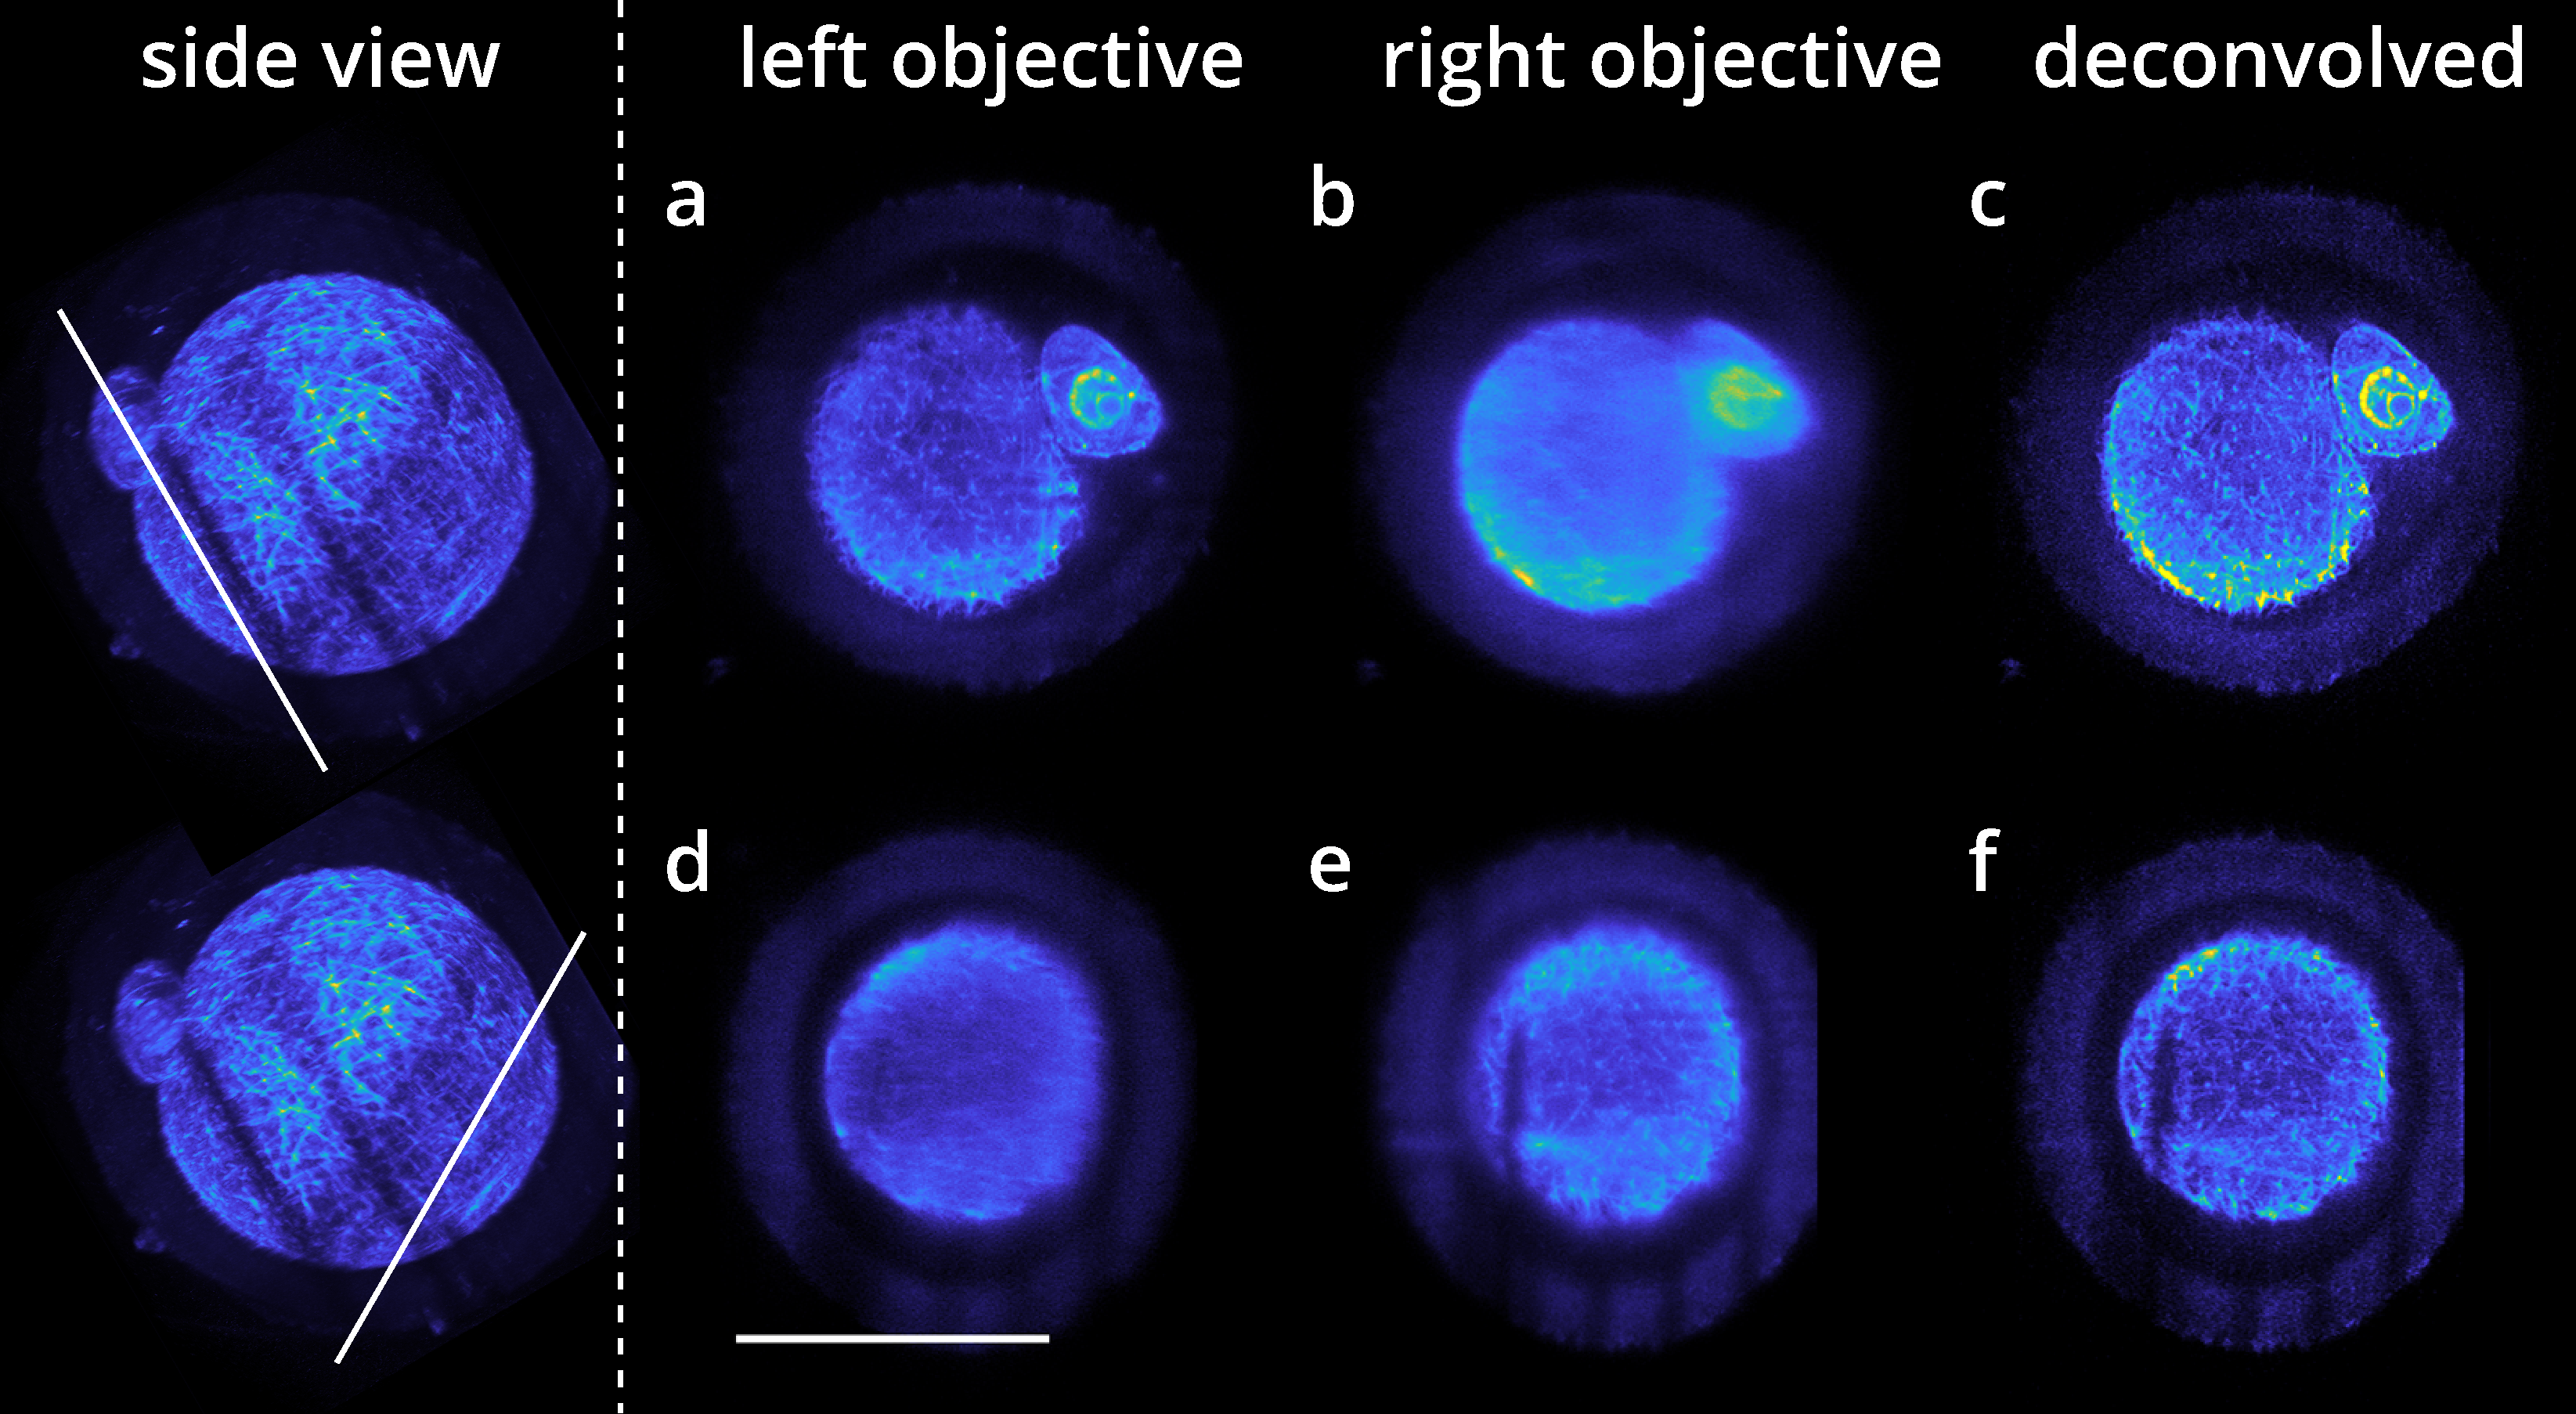
\includegraphics[width=.75\textwidth]{zygoteMontage}
      \bcaption[Multi-view recording of a mouse zygote]{Dual-view imaging was performed on a fixed mouse zygote. Microtubules wre stained with Alexa Fluor 488. Top row: view of Left objective. Bottom row: view of Right objective. (a) Raw image from left objective. (b) Rotated view of Right objective. (c) Multi-view deconvolution of stacks (a) and (b). (d) Rotated slice from left objective. (e) Raw image from right objective. (f) Multi-view deconvolution of stacks (d) and (e). Scale bar: \SI{50}{\micro m}.}
      \label{fig:zygoteMontage}
    \end{figure}

    To demonstrate the multi-view capabilities and improved image quality of the microscope, we performed dual-view imaging of a fixed mouse zygote and combined the images using the Multiview Reconstruction \cite{preibisch_efficient_2014} plugin of Fiji (\autoref{fig:zygoteMontage}). The microtubules were stained with Alexa Fluor 488, and the zygote was imaged from both views with \SI{0.5}{\micro m} inter-plane distance.

    Anisotropy in the resolution becomes apparent in the single-view recordings, when the stacks are resliced from a different direction than the imaging plane. Even though the native view of each objective (\autoref{fig:zygoteMontage}a,d) shows good contrast, and easy to recognize features, when rotated and sliced corresponding to the view of the other objective, the contrast is almost completely gone, and resolution is decreased (\autoref{fig:zygoteMontage}b,e). The fused stack, after the multi-view deconvolution contains the high resolution information form both views, and thus both directions show good quality and high contrast (\autoref{fig:zygoteMontage}c,f).

    



    %#     ## ######## ######## ##     ## 
    %##   ### ##          ##    ##     ## 
    %### #### ##          ##    ##     ## 
    %# ### ## ######      ##    ######### 
    %#     ## ##          ##    ##     ## 
    %#     ## ##          ##    ##     ## 
    %#     ## ########    ##    ##     ## 

\section{Methods}
    \label{sec:methods2}

  \subsection{Preparation of fluorescent bead samples}
    For registration and resolution measurements we used TetraSpeck \SI{0.5}{\micro m} diameter fluorescently labeled beads (ThermoFisher, T7281). The stock bead solution was thoroughly vortexed and sonicated for \SI{5}{min} before diluting it 1:100 in distilled water. The diluted bead solution saw stored at \SI{4}{\degree C} until use. GelRite (Sigma-Aldrich, G1910) gel was prepared in distilled water at 0.8\% concentration with 0.1\% $\mathrm{MgSO_4\cdot 7 H_2O}$ and kept at \SI{70}{\degree C} until use. \SI{50}{\micro l} of the diluted bead solution was added with a heated pipette tip to \SI{450}{\micro l} of gel solution at \SI{70}{\degree} to prevent  polymerization. The gel was thoroughly vortexed, and loaded to glass micropipettes (Brand \SI{100}{\micro l}). The gel was allowed to cool to room temperature and stored in a petri dish under $\mathrm{dH_2O}$ at \SI{4}{\degree} until use. For imaging, a small piece of gel was extruded from the capillary, cut off, and placed in the sample holder. After positioning the gel to the bottom of the sample holder, the holder was filled with \SI{200}{\micro l} $\mathrm{dH_2O}$.

  \subsection{Preparing the sample holder}
    The sample holder was lined with \SI{12.5}{\micro m} (PSF measurements) or \SI{50}{\micro m} (mouse zygote and \textit{Drosophila} embryo imaging) thin FEP foil ( "BRAND" ). The FEP foils were cut to size, washed with 70\% ethanol followed by a second wash with $\mathrm{dH_2O}$. After washing, both surfaces of the foils were chemically activated by a \SI{20}{s} plasma treatment ( "MACHINE" ). The foils were then stored in a petri dish until further use separated by lens cleaning tissues (Whatman, 2105-841
    ). Before imaging, the sample holder was cleaned with dish soap, rinsed with tap water, rinsed with 70\% ethanol, and rinsed with $\mathrm{dH_2O}$. The prepared foils were glued to the inside of the cleaned sample holder with medical grade silicon glue ( "BRAND" ). During the \SI{5}{min} curing process the foil was pressed against the sample holder by a custom made press fitting the shape of the sample holder. Final dilution of the stock bead solution in the gel is 1:1000.

  \subsection{Drosophila embryo imaging}
    \textit{Drosophila melanogaster} embryos (fly stock AH1) expressing fluorescent nuclear (H2A-mCherry) and centriole (ASL-YFP) markers were collected on an agar juice plates and dechorionated in 50\% bleach solution for \SI{1}{min}. After rinsing the bleach with deionized water, the embryos were placed in the sample holder under PBS solution. A small piece of gel containing fluorescent beads were also placed next to the samples to aid in multi-view registration.

  \subsection{Mouse zygote imaging}
    Fixed mouse zygotes labeled with Alexa-488 (microtubules) and Alexa-647 (kinetochores) were kindly provided by Judith Reichmann. Zygotes were transferred to the sample holder, and imaged in PBS. To allow for multi-view reconstruction, a fluorescent beads (TetraSpeck \SI{0.5}{\micro m} suspended in GelRite wre placed next to the zygote in the sample holder. After imaging the zygote from both views, the beads were also recorded using the same stack definitions. After data acquisition, the multi-view datasets were registered and deconvolved in Fiji \cite{schindelin_fiji:_2012} using the Multiview Reconstruction Plugin \cite{preibisch_software_2010,preibisch_efficient_2014}. The deconvolution was based on a simulated PSF generated in Fiji with the PSF Generator plugin \cite{kirshner_3d_2011} using the Born-Wolf PSF model \cite{born_principles_2013}. $\mathrm{NA_{ex}}=0.1$, $\mathrm{NA_{em}}=1.1$, n=1.33, $\lambda_{ex} = \SI{488}{nm}$, $\lambda_{em} = \SI{510}{nm}$.

  

  % \subsection{Drosophila salivary gland imaging}
  %   Salivary glands from third instar larvae expressing fluorescent nuclear (H2A-mCherry) and centriole (ASL-YFP) markers were kindly provided by Ulla-Maj Fiuza. The salivary glands were imaged in PBS, together with a small piece of gel with fluorescent beads.


% !TEX root = dissertation_BB.tex
%% spellcheck-language en-US

%    #
%   #
%  #  #
%  #####
%     #

\chapter{Real-time, GPU accelerated image processing pipeline}

\graphicspath{{./figures/4_gpu/}}


\section{Challenges in data handling for light-sheet microscopy}

  When using any kind of microscopy in research, image processing is a crucial part of the workflow. This is especially true for light-sheet microscopy, since it is capable of imaging the same specimen for multiple days, producing immense amounts of data. A single overnight experiment of \textit{Drosophila} development (which is a very typical use-case for light-sheet) can produce multiple terabytes of data.

  Apart from light-sheet microscopy, many other microscopy modalities are also suffering from this problem. Methods, such as high content screening \cite{carpenter_systematic_2004,echeverri_high-throughput_2006,pepperkok_high-throughput_2006}, where tens of thousands of different genotypes are imaged generating millions of images; and single molecule localization microscope (SMLM) \cite{betzig_imaging_2006,hess_ultra-high_2006,rust_sub-diffraction-limit_2006}, where just a single plane of a single sample is imaged hundreds of thousands of times to acquire super-resolved images.

  Not only these methods are capable of generating data extremely fast, but with the sustained high data rate a single experiment can easily reach multiples of terabytes (\autoref{fig:sizes}). Handling this amount of data can quickly become the bottleneck for many discoveries, which is a more and more common issue in biological research \cite{wollman_high_2007,reynaud_guide_2015,perkel_struggle_2016}. 


  \begin{figure}[btp]
    \centering
    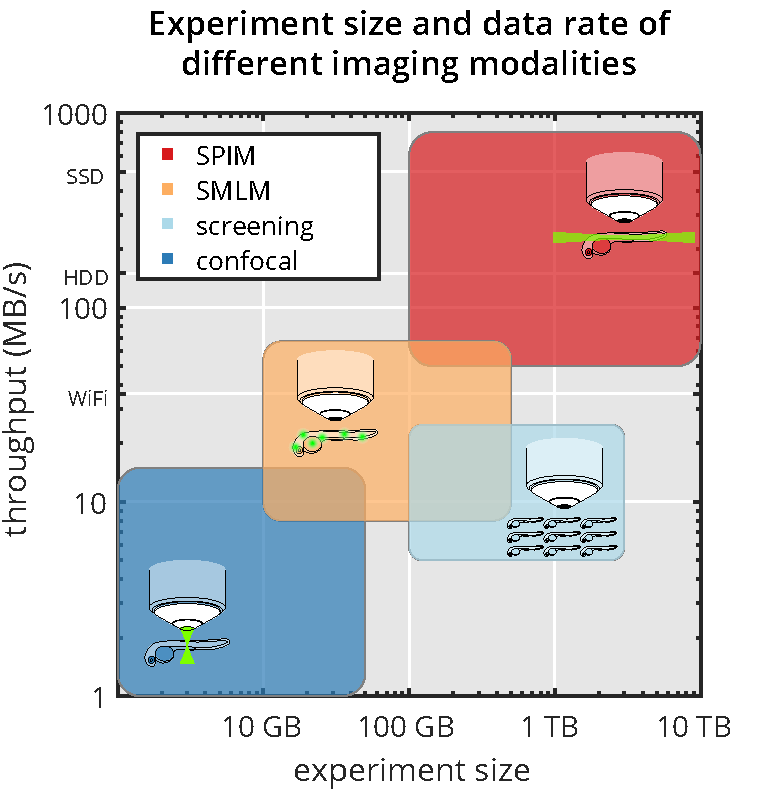
\includegraphics[page=1,width=0.5\textwidth]{comparison_with_pictograms}
    \bcaption[Experiment sizes and data rate of different imaging modalities]{Comparison of single-plane illumination microscopy (SPIM, red rectangle), high-content screening (light blue), single molecule localization microscopy (SMLM, orange) and confocal microscopy (blue) by typical experiment size and data production rate (see also Table \ref{tab:sizes}).}
    \label{fig:sizes}
  \end{figure}

  % To efficiently and quickly process such amounts of information, developing new strategies / innovative approaches is indispensible. As image processing tasks are typically highly parallelizable 

  This chapter will focus on addressing these challenges, by presenting a real-time, GPU-based image preprocessing pipeline consisting of two parts (\autoref{fig:pipeline}).
  The first part is a fast image fusion method for our workhorse light-sheet microscope, the MuVi-SPIM \cite{krzic_multiview_2012}, that enables live fusion of the images arriving from two opposing cameras.
  The second part of the pipeline, which can also be used in a standalone way, is a real-time image compression library that allows lossless and within noise level compression of the data already during acquisition.

  \begin{figure}
    \centering
    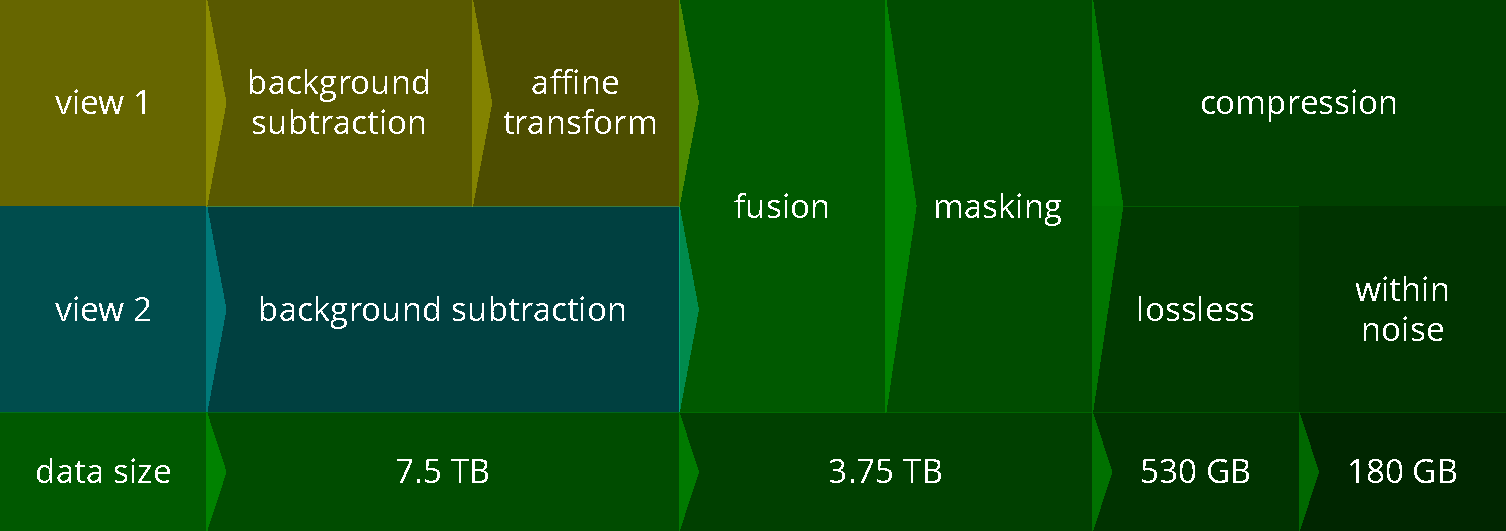
\includegraphics[width=\textwidth]{pipeline}
    \bcaption[Real-time image processing pipeline for multi-view light-sheet microscopy]{}
    \label{fig:pipeline}
  \end{figure}



  \subsection{CUDA architecture}

    CUDA \cite{nickolls_scalable_2008}
    CUDA programming Guide \cite{nvidia_cuda_2015}



    % ######## ##     ##  ######  ####  #######  ##    ## 
    % ##       ##     ## ##    ##  ##  ##     ## ###   ## 
    % ##       ##     ## ##        ##  ##     ## ####  ## 
    % ######   ##     ##  ######   ##  ##     ## ## ## ## 
    % ##       ##     ##       ##  ##  ##     ## ##  #### 
    % ##       ##     ## ##    ##  ##  ##     ## ##   ### 
    % ##        #######   ######  ####  #######  ##    ## 

\section{Live fusion}

Similarly to the DualMouse-SPIM, our currently used production microscope, the Multiview-SPIM (MuVi-SPIM) \cite{krzic_multiview_2012} also uses multiple imaging directions to improve the image quality. In this case, however, the aim is completeness rather than increasing the resolution. As the MuVi-SPIM is capable of imaging much larger specimens, such as entire \textit{Drosophila} embryos, the sample size itself can present some challenges, especially for opaques specimens. As light scattering and absorption impacts both the illumination and detection optics, the negative effects for SPIM are more pronounced compared to single-lens systems \cite{de_medeiros_deep_2016}.




\subsection{Multiview SPIM for \textit{in toto} imaging}

MuVi-SPIM  provides an elegant solution for multi-view imaging. A standard SPIM setup with a single detection and a single illumination lens would rotate the sample to acquire images from multiple directions. MuVi-SPIM, on the other hand, utilizes two opposing objectives for illumination, and two opposing objectives for detection (\autoref{fig:muvi-spim}a). As the sample is held by an aqueous gel inside the imaging chamber, all objectives have unobstructed view of it from multiple directions (\autoref{fig:muvi-spim}b,c).

Data acquisition is done in two steps: the sample is illuminated by Light sheet 1, and fluorescence is collected by both detection objectives at the same time, after which Light sheet 2 is activated, and both cameras record the fluorescence again (\autoref{fig:muvi-spim}d). This process will result in 4 datasets, all with partial information due to scattering effects. The 4 views are later fused to a single, high quality dataset (\autoref{fig:muvi-spim}e). This fusion process is necessary before any further analysis steps can be performed, however due to the sheer size of the data, it takes a considerable amount of time after the acquisition.

By combining scanned light-sheet \cite{keller_reconstruction_2008} with confocal slit detection on the camera chip \cite{baumgart_scanned_2012}, it is possible to exclude out of focus, scattered illumination light. This way it is  possible to illuminate simultaneously with both light-sheets, which leaves us with only two views, the views of the two opposing cameras \cite{de_medeiros_confocal_2015}.

\begin{figure}
  \centering
  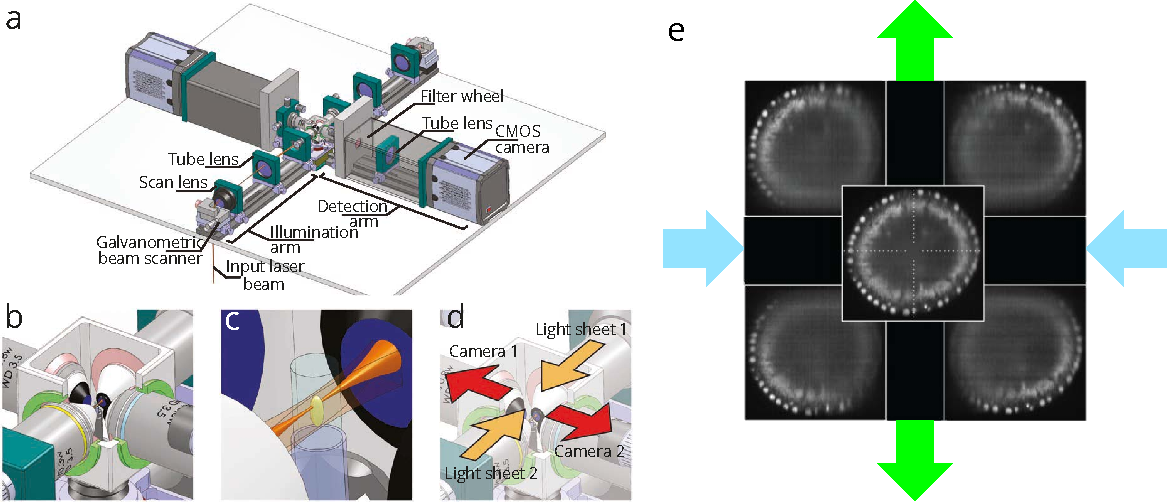
\includegraphics[width=1\columnwidth]{fusion/muvi-spim}
  \bcaption[Operating principle of MuVi-SPIM]{(a) The microscope consists of two illumination and two detection arms for simultaneous multi-view illumination and detection. (b) The 4 arms meet in the imaging chamber that is filled with water, and contains the sample. (c) The sample is held by a glass capillary, in  a GelRite cylinder. Optical sectioning is acheived by a virtaul light-sheet. (d) The light-sheets can be generated from two sides (Light sheet 1 and 2), and detection is also double sided (Camera 1 and 2). Adapted from \cite{krzic_multiview_2012}.}
  \label{fig:muvi-spim}
\end{figure}

\begin{figure}
  \centering
  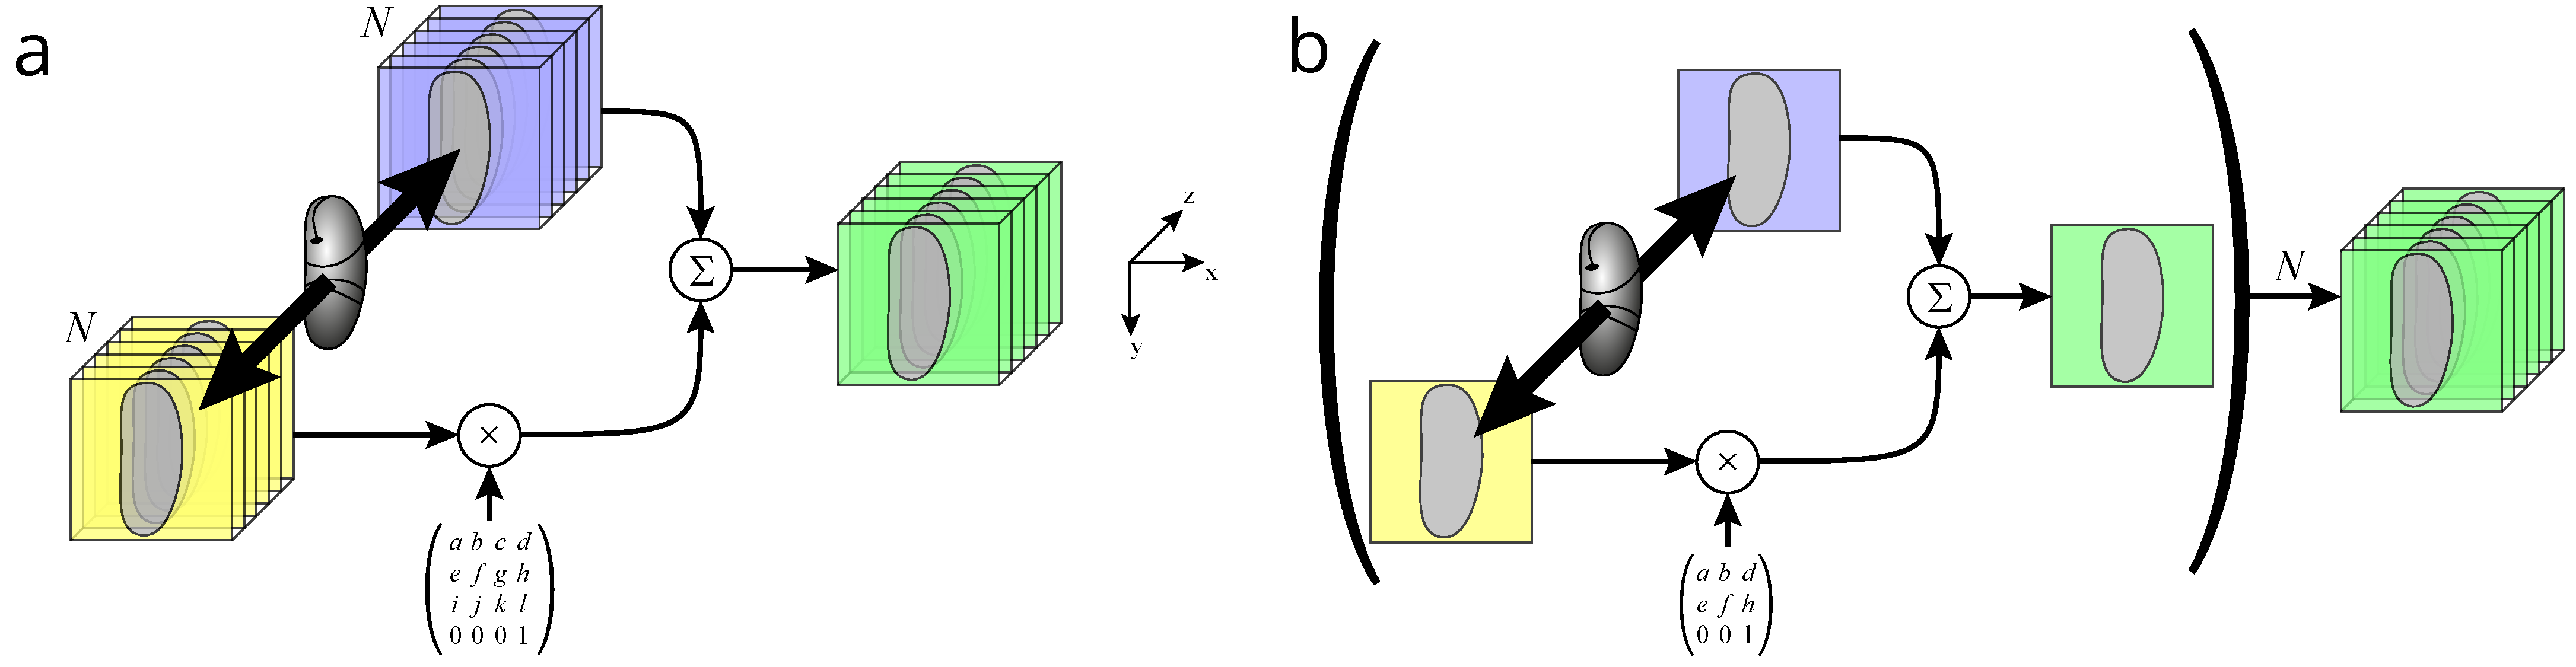
\includegraphics[width=1\columnwidth]{fusion/acquisition}
  \bcaption[Multi-view fusion methods for light-sheet microscopy]{a) Full 3D stacks are acquired from the opposing views (yellow and blue), which are then registered in 3D space using previously acquired affine transformation parameters. Registered stacks are then weighted averaged to create the final fused stack (green). b) Images from opposing views are directly fused plane by plane. Registration takes place in 2D space thus reducing computational effort and memory requirements. The registered planes are then weighted averaged to create the final fused image.}
  \label{fig:acquisition}
\end{figure}


\subsection{Image registration}
To perform image fusion of multiple views, first image registration is necessary: the coordinate systems of both views have to be properly overlapped. Ideally a single mirroring transformation would be enough to superpose the two camera images, however in practice the microscope can never be aligned with such precision. Other types of transformations are also necessary: translation to account for offsets in the field of view; scaling in case of slightly different magnifications; and also shearing if the detection plane is not perfectly perpendicular to the sample movement direction. To combine all of these effects, a full 3D affine transformation is necessary to properly align the two camera images (Fig. \ref{fig:acquisition} a). This transformation can be represented by a matrix multiplication with 12 different parameters:
\[
\begin{pmatrix}
a & b & c & d \\ 
e & f & g & h \\ 
i & j & k & l \\
0 & 0 & 0 & 1 
\end{pmatrix}
\times
\begin{pmatrix}
x\\
y\\
z\\
1
\end{pmatrix}
=
\begin{pmatrix}
a x + b y + c z + d\\ 
e x + f y + g z + g\\ 
i x + j y + k z + l\\
1
\end{pmatrix}
\]
where $x, y, z$ are the coordinates of the original 3D image, and $a, b, c, d, e, f, g, h, i, j, k, l$ are the affine transformation parameters.

These parameters are traditionally acquired by imaging fluorescent beads suspended in a gel cylinder. The bead recordings are segmented, matching beads are automatically detected in each camera view, and using the RANSAC method the affine transformation parameters are determined. For two opposing views these parameters are only dependent on the optical setup itself, and not the sample or the experiment. Because of this, it is sufficient to determine the transformation parameters only after modifying/realigning the microscope.

This method of fusion however is quite cumbersome for the average user. The raw data is made up of two stacks, each of which only has one half with high contrast.
To evaluate the experiment, the user either has to look at both recordings, or wait for the offline fusion to complete, and examine the result.

It would be much more practical to already fuse the opposing views before displaying or saving the image. Since the two cameras ideally image the same $z$ plane, it should be possible to reduce the alignment problem to a 2D affine transformation:
\[
\begin{pmatrix}
a & b & d\\ 
e & f & h \\
0 & 0 & 1
\end{pmatrix}
\times
\begin{pmatrix}
x\\
y\\
1
\end{pmatrix}
=
\begin{pmatrix}
a x + b y + d\\ 
e x + f y + g\\
1
\end{pmatrix}
\]
If this is possible, then fusion can be carried out separately for each image plane (Fig. \ref{fig:acquisition} b), which would greatly facilitate live image fusion. The requirements for this are the following:
\begin{align}
\left| c z \right| &< \sigma_{xy} & \forall z \label{eq:req1}\\
\left| g z \right|  &< \sigma_{xy} & \forall z \label{eq:req2}\\
\left| i x + j y + (k-1)  z + l \right| &< \sigma_z & \forall x, y, z  \label{eq:req3}
\end{align}
where $\sigma_{xy}$ is the lateral resolution, and $\sigma_z$ is the axial resolution of the microscope, which are 277 nm and 1099 nm respectively. 

 If these conditions hold (\textit{i.e.} the microscope is properly aligned), then direct plane by plane fusion will not result in any loss of information compared to the full 3D image fusion.

% \subsection{Image preprocessing pipeline}

% \begin{figure}[bth]
% \centering
% \includegraphics[width=0.4\columnwidth]{fusion/pipeline}
% \caption{Image preprocessing pipeline. The pipeline comprises of two parts: processing on CPU (white background) and processing on GPU (green background). Images are first transferred from the CPU to the GPU, where the preprocessing steps take place. These include background subtraction, affine transformation, weighted averaging and optionally thumbnail generation and image compression. After the preprocessing steps the image is transferred back to the CPU, and saved on the hard drive, or streamed to a remote computer. Data sizes after each preprocessing step are shown in the gray bands for planes, stacks and time-lapses.}
% \label{fig:pipeline}
% \end{figure}

% To perform the image fusion step as fast as possible, thus enabling it is use for live imaging, we used CUDA (Compute Unified Device Architecture) \cite{_cuda_????-1} to implement the algorithm on a graphics card (NVIDIA, GTX 750). This architecture offers a convenient way to harness the massively parallel computing capabilities of the many streaming multiprocessors residing on a GPU (graphics processing unit). Since each processing step we require is pixel based, they can be inherently parallelized to gain tremendous advantage in computing time.

% To utilize the GPU for the image processing step, the images first have to be transferred from the computer main memory to the graphics card memory. Because of the limited bandwidth of the PCIe 2.0 16x bus, this step is actually the bottleneck, and not the computation itself. To optimize data transfer speed, several techniques can be used.

% First, one has to make sure that the space for the original image data is allocated as paged-lock memory. This is possible with \texttt{cudaMallocHost}. This function will make sure that the memory space allocated on the host will be page-locked \textit{i.e.} it is contents cannot be temporarily swapped to the pagefile on the hard disk, and it is actually mapped to the physical memory. Otherwise, with normal allocation functions this is not guaranteed by the operating system, and the memory is only mapped to the physical memory when it is contents are accessed, which heavily influence read/write speed.

% Second, if the same operation is carried out for many images (as in the case of our live fusion method), the data transfer for the next image can already be carried out while the previous image is being processed, thus masking at least one of the data transfers between the main memory and the graphics card.

% % Even when using both methods, most of the time is still taken by the data transfer. Because of this, we decided to implement additional image preprocessing steps in our pipeline (Fig \ref{fig:pipeline}, thus ...

% %To maximize GPU utilization, and ultimately justify the long data transfer times, in addition to the plane by plane fusion (which is actually an affine transformation followed by weighted average), we also implemented background subtraction, subsampling, LUT conversion from 16 bits to 8 bits, and JPEG compression in our pipeline (Fig \ref{fig:pipeline}). All of these steps either enhance image quality (such as background subtraction), reduce data size (LUT conversion, subsampling, JPEG), or both (fusion).

% Since our microscope control software is implemented in LabVIEW, all the functions in our pipeline were incorporated in a dynamic linked library (DLL) which can be loaded by LabVIEW to use the CUDA functions. Furthermore, to facilitate the integration to existing software, we created a LabVIEW library based on these CUDA functions, to provide a consistent and easy to use interface for further development.

\subsection{Results}

\begin{figure*}[tb]
\centering
\includegraphics[width=1\textwidth]{fusion/drosophila_D2}
\caption{ GPU fused images of a \textit{Drosophila melanogaster} embryo. Two stacks were taken in quick succession first without fusion, then with fusion enabled. Fused images are shown in the middle of each subfigure, while the individual camera images are in the bottom insets. The top-left inset depicts the z-position of the shown images. a) Image from closer to the left camera. b) Image from the center of the embryo. c) Image from closer to the right camera.}
\label{fig:drosophila}
\end{figure*}

The image preprocessing pipeline was tested on our previously described Multi-View Single Plane Illumination Microscope (MuVi-SPIM)\cite{krzic_multiview_2012}. For the background subtraction we recorded 1500 dark images with each camera and averaged them, to obtain the camera specific background images. Before image acquisition these were uploaded to the GPU memory, and were readily available for the pipeline.

After careful alignment of the microscope to meet the previously discussed requirements (Eqs. \eqref{eq:req1} -- \eqref{eq:req3}), we imaged fluorescent beads in a gel suspension to obtain the affine transformation parameters. After making sure that these parameters indeed fulfill the previously set requirements, these were also uploaded to the GPU memory for further use in our pipeline.

To validate our hypotheses, that 2D direct image fusion is sufficient instead of the full 3D fusion, we image several samples. First, we imaged the flourescent beads again, now with the live fusion enabled, to make sure our registration parameters are correct. Manual evaluation of the data revealed that the fusion indeed worked, without any artifacts, such as double beads which would indicate an imprecision in alignment or in the transformation parameters.

We also applied the live fusion to a real biological specimen, namely \textit{Drosophila melanogaster} embryos expressing H2Av-mCherry histone marker. The embryos were imaged first without direct fusion enabled, and immediately afterwards with direct fusion enabled (Fig. \ref{fig:drosophila}). Image quality dependency on the depth of the imaging plane is especially apparent in single-view stacks. Planes closer to the camera give a sharp, high contrast image, while planes further then the middle of the embryo are severely degraded due to scattering.

Stacks obtained with the live fusion enabled show a consistently high image quality throughout the entire stack, independent of the depth. This allows us to keep only the already fused data, thus effectively reducing the storage requirement by half, and facilitating further data processing steps. 


% \section{Conclusions}
% In this report I described a universal light-sheet microscope control software that will be used for the symmetric mouse SPIM setup. This software is already used by our other microscopes, including the mouse SPIM developed by Petr Strnad, and the LS-RESOFLT microscope by Patrick Hoyer. Papers on both of these have been submitted to Nature Methods.

% I also developed a direct plane by plane fusion method which was implemented in CUDA, and can be performed live, directly on the microscope. This results in a single, high quality recording, which can be directly used later for further processing or data evaluation. We showed the viability of the method by imaging fluorescent beads, and fluorescently labeled \textit{Drosophila m.} embryos, which showed superior image quality to both of the original views. As a further consequence, data handling became easier, less storage is needed for further experiments, and considerable time is spared by eliminating the need for the 3D fusion step.

% Despite the many advantages, further development is still necessary. A natural next step is to add compression to the pipeline to further reduce data sizes. For several samples orthogonal views are desired, or in some cases the optical setup is already designed with orthogonal detection\cite{wu_spatially_2013}, or close to orthogonal in the case of the symmetric mouse SPIM. In these cases to properly fuse the different directions, multi-view deconvolution is necessary \cite{krzic_multiple-view_2009,temerinac-ott_multiview_2012} to gain maximum information from both views.






%#######   #######  ########  
%#     ## ##     ## ##     ## 
%#     ##        ## ##     ## 
%#######   #######  ##     ## 
%#     ##        ## ##     ## 
%#     ## ##     ## ##     ## 
%#######   #######  ########  
  
\section{\b3d image compression}

  The second part of our GPU-based image preprocessing pipeline is a new image compression algorithm that allows for extremely fast image compression to efficiently reduce data sizes already during acquisition.
  
  

  A straightforward solution to these problems would be to compress the images during acquisition. Although this would not reduce the requirements for image processing power and time, it still has a big impact on the necessary background infrastructure. By reducing the data size, not only the cost for storage can be reduced, but the time it takes to transfer the data during the various steps of data processing. A fast compression method would also greatly improve 3D data browsing possibilities, as more data could be piped to the rendering software.

  Despite these advantages, not many microscopists have implemented real time compression strategies during acquisition, and this is mostly due to the lack of appropriate compression methods suitable for scientific imaging that also offers the high throughput demanded by these applications. Typically used lossless compression methods, such as JPEG2000 \cite{adams_jpeg-2000_2001} although offer good compression ratios, are very slow in processing speed, at least compared to the data rate of a modern microscope ($\sim \SI{1}{GB/s}$). High speed compression methods that could deal with this data rate have been developed for ultra high definition 4K and 8K digital cameras, such as the high efficiency video codec (HEVC) \cite{international_telecommunications_union_h.265_2016}. These methods, however, have been optimized for lossy image compression which is generally not acceptable for scientific data \cite{cromey_digital_2013}, and rarely support compression of high bit rate originals, which is typically the case for modern sCMOS sensors. Although the HEVC recommendation does specify bit rates up to 16 bits, and lossless compression, we

  To address these issues, we developed \b3d, a GPU based image compression method that is capable of high speed compression of microscopy images during the image acquisition process. By utilizing the massively parallel processing architecture of a GPU, we were not only able to reach a compression and decompression speed of \SI{1}{GB/s}, but our algorithm also keeps the load off the CPU, making it available for other computing tasks related to operating the microscope itself.

  A second feature of our compression library is a novel algorithm for noise dependent lossy compression of scientific images. As mentioned before, lossy compression is not recommended for scientific images, and the reason for this, is all practical lossy compression algorithms are designed with the intent of fooling the human visual system \cite{sayood_introduction_2012}. While the images compressed by these algorithms may appear identical to the eye, any downstream data analysis could be negatively impacted by the compression artifacts. To our knowledge, only a single algorithm allows to set the loss in a deterministic manner: the near-lossless operating mode of JPEG-LS \cite{weinberger_loco-i_2000}. In this mode it is possible to set the maximum allowable error a pixel can have after decompression. Although this can be useful for certain applications, it has not been widely implemented, as the visual quality loss is more severe compared to other algorithms with the same compression ratio \cite{santa-cruz_study_2000}.

  \b3d image compression
  light-sheet (Sec. \ref{sec:light-sheet})
  data handling is bottleneck 

  KLB \cite{amat_efficient_2015}

  big data viewer \cite{pietzsch_bigdataviewer:_2015}
  Fiji \cite{schindelin_fiji:_2012}

  FLIC \cite{wang_fast_2012}
  SFALIC \cite{starosolski_simple_2007}
  FELICS \cite{howard_fast_1993} -> this was before JPEG-LS
  Treib terrain editing \cite{treib_interactive_2012}
  Treib turbulence \cite{treib_turbulence_2012}



    


    

  \subsection{Compression algorithm}

    compression scheme: modeling+ coding \cite{rissanen_universal_1981}

    \begin{figure}[tpb]
      \centering
      \includegraphics[page=1,width=0.6\textwidth]{SFig1_flow}
      \bcaption[\b3d algorithm schematics]{(\textbf{a}) Prediction context for pixel X, the next sample to be encoded. Three neighboring pixels are considered: left (A), top (B) and top left (C) neighbors. (\textbf{b}) Lossless JPEG predictors for X, based on the context showed in (\textbf{a}). The first three predictors are one-dimensional, while the rest are two-dimensional. Using a two dimensional predictor while increases complexity slightly, also increases the achievable compression ratio. We found that for fluorescence microscopy images predictor 7 performs best, hence its inclusion in the \b3d algorithm. (\textbf{c)} Complete algorithm flowchart depicting the main stages of the compression. First, if the result should be lossless, pixel prediction is performed on the original image values. If within noise level mode is selected, the image noise is stabilized first (see "\textbf{Supplementary Note}"), which is then scaled by the quantization step q. Prediction is performed, and the prediction errors are rounded to the nearest integer. The prediction errors for both lossless and lossy modes are then run-length encoded, and finally Huffman coding is applied to effectively reduce data size. The output of the Huffman coder is saved as the compressed file.}
      \label{fig:algorithm}
    \end{figure}



    \begin{figure}[tpb]
      \centering
      \includegraphics[page=1,height=0.5\textwidth]{bubbles}
      \bcaption[Lossless compression performance]{Performance comparison of our \b3d compression algorithm (red circle) vs. KLB (orange), uncompressed TIFF (light yellow), LZW compressed TIFF (light blue) and JPEG2000 (blue) regarding write speed (horizontal axis), read speed (vertical axis) and file size (circle size). (see also Table \ref{tab:performance}).}
      \label{fig:performance}
    \end{figure}

    

    \begin{figure}[tpb]
      \centering
      \includegraphics[page=1,width=0.7\textwidth]{swapping}
      \bcaption[Options for noise dependent lossy compression]{Comparing Mode 1 (prediction then quantization) and Mode 2 (quantization then prediction) of noise dependent lossy compression in terms of compression ratio, peak signal to noise ratio (PSNR) and spatial correlations introduced to random noise. (\textbf{a}) Compression ratio as a function of the quantization step for Mode 1 and Mode 2. (\textbf{b}) PSNR as a function of the quantization step for Mode 1 and Mode 2. (\textbf{c, d}) Random noise was compressed at various quantization steps both for Mode 1 and Mode 2. Autocorrelation was calculated for the compressed images to see whether the compression introduces any spatial correlation between the pixels. For q=1$\upsigma$ both modes are free of correlation (\textbf{c}, top: compressed images, bottom: autocorrelation), however, for q=2$\upsigma$ Mode 1 exhibits a correlation pattern (\textbf{d}, top left: compressed image, bottom left: autocorrelation) that is not present in Mode 2 (\textbf{d}, top right compressed image, bottom right: autocorrelation). For more discussion, see "\textbf{Supplementary Note}".}
      \label{fig:swapping}
    \end{figure}

  \subsection{Benchmarking}

    \begin{figure}[tpb]
      \centering
      \includegraphics[page=1,height=0.5\textwidth]{Fig1c_compressionBars}
      \bcaption[Within noise level compression performance]{WNL compression performance compared with lossless performance for 9 different dataset representing 3 imaging modalities (SPIM, SMLM, screening). Compression ratio = original size / compressed size. For description of datasets see Table \ref{tab:datasets} in Appendix B.}
      \label{fig:benchmark}
    \end{figure}

    \begin{figure}[tpb]
      \centering
      \includegraphics[page=1,width=0.9\textwidth]{wnlSamples}
      \bcaption[Image quality of a WNL compressed dataset]{WNL compression performance compared with lossless performance for 9 different dataset representing 3 imaging modalities (SPIM, SMLM, screening). Compression ratio = original size / compressed size. For description of datasets see Table \ref{tab:datasets}.}
      \label{fig:wnlSamples}
    \end{figure}

    \begin{figure}[tpb]
      \centering
      \includegraphics[page=1,width=0.7\textwidth]{SFig4_RMSDvsSD}
      \bcaption[Compression error compared to image noise]{To compare the difference arising from WNL compression to image noise, we imaged a single plane 100 times in a \textit{Drosophila melanogaster} embryo expressing H2Av-mCherry nuclear marker at \SI{38}{ms} intervals. The whole acquisition took \SI{3.8}{s}, for which the sample can be considered stationary. To visualize image noise, the standard deviation was calculated for the uncompressed images (left). All images were then WNL compressed, and the root mean square deviation was calculated compared to the uncompressed images (right). The root mean square deviation on average is 3.18 times smaller than the standard deviation of the uncompressed images.}
      \label{fig:RMSD}
    \end{figure}

    

    \begin{figure}[tpb]
      \centering
      \includegraphics[page=1,width=1\textwidth]{LLvsB3D}
      \bcaption[Influence of noise dependent lossy compression on 3D nucleus segmentation]{A \textit{Drosophila melanogaster} embryo expressing H2Av-mCherry nuclear marker was imaged in MuVi-SPIM \cite{krzic_multiview_2012}, and 3D nucleus segmentation was performed ( "\textbf{Online Methods}") (\textbf{a}). The raw data was subsequently compressed at increasingly higher compression levels, and segmented based on the training of the uncompressed data. To visualize segmentation mismatch, the results of the uncompressed (green) and compressed (magenta) datasets are overlaid in a single image (\textbf{b}, \textbf{c}; overlap in white). Representative compression levels were chosen at two different multiples of the photon shot noise, at q=1$\upsigma$ (\textbf{b}) and q=4$\upsigma$ (\textbf{c}). For all compression levels the segmentation overlap score ( "\textbf{Online Methods}") was calculated and is plotted in (\textbf{g}) along with the achieved compression ratios.}
      \label{fig:wnlDroso}
    \end{figure}

    \begin{figure}[tpb]
      \centering
      \includegraphics[page=3,width=1\textwidth]{LLvsB3D}
      \bcaption[Influence of noise dependent lossy compression on 3D membrane segmentation]{A \textit{Phallusia mammillata} embryo expressing PH-citrine membrane marker was imaged in MuVi-SPIM \cite{krzic_multiview_2012}, and 3D membrane segmentation was performed ( "\textbf{Supplementary Methods}") (\textbf{a}). The raw data was subsequently compressed at increasingly higher compression levels, and segmented using the same settings as the uncompressed data. To visualize segmentation mismatch, the results of the uncompressed (green) and compressed (magenta) datasets are overlaid in a single image (\textbf{b, c}; overlap in white). Representative compression levels were chosen at two different multiples of the photon shot noise, at q=1.6$\upsigma$ (\textbf{b}) and q=4.8$\upsigma$ (\textbf{c}). For all compression levels the segmentation overlap score ( "\textbf{Supplementary Methods}") was calculated and is plotted in (\textbf{d}) along with the achieved compression ratios.}
      \label{fig:wnlPhallusia}
    \end{figure}

    \begin{figure}[tpb]
      \centering
      \includegraphics[page=2,width=1\textwidth]{LLvsB3D}
      \bcaption[Influence of noise dependent lossy compression on single-molecule localization]{Microtubules, immunolabeled with Alexa Fluor 647 were imaged by SMLM (\textbf{a}). The raw data was compressed at increasingly higher compression levels, and localized using the same settings as the uncompressed data. To visualize localization mismatch, the results of the uncompressed (green) and compressed (magenta) datasets are overlaid in a single image (\textbf{b}, \textbf{c}; overlap in white). Two representative compression levels were chosen at q=1$\upsigma$ (\textbf{b}) and q=4$\upsigma$ (\textbf{c}). To assess the effects of compression on localization precision, a simulated dataset with known emitter positions was compressed at various levels. For all compression levels the relative localization error (normalized to the Cramér–Rao lower bound) was calculated and is plotted in (\textbf{d}) along with the achieved compression factors.}
      \label{fig:wnlSMLM}
    \end{figure}

    \begin{figure}[tpb]
      \centering
      \includegraphics[page=1,width=0.5\textwidth]{SFig6_locprecVsNphotons}
      \bcaption[Change in localization error only depends on selected quantization step]{We simulated multiple datasets ( "\textbf{Supplementary Methods}") with different average photon numbers per localization. Background was kept at a constant average of 20 photons/pixel. Datasets were compressed at multiple compression levels (see legend), and localization error relative to the Cramér-Rao lower bound was calculated. The relative localization error only depends on the compression level, and not on the signal to background illumination ratio.}
      \label{fig:SFig6_locprecVsNphotons}
    \end{figure}



\section{Noise dependent lossy compression}
  
  square root compression \cite{gowen_square_2003}
  noise and bias in square root compression \cite{bernstein_noise_2010}
  quantization \cite{gray_quantization_1998}
  Anscombe \cite{anscombe_transformation_1948}
  optimal inverse Anscombe \cite{makitalo_optimal_2011,makitalo_closed-form_2011}
  optimal inverse generalized Anscombe \cite{makitalo_optimal_2013}

\section{Methods}
  
\subsubsection{Compression benchmarking}
For all presented benchmarks, TIFF and JPEG2000 performance was measured through MATLAB's imwrite and imread functions, while KLB and \b3d performance was measured in C++. All benchmarks were run on a computer featuring 32 processing cores (2×Intel Xeon E5-2620 v4), \SI{128}{GB} RAM and an NVIDIA GeForce GTX 970 graphics processing unit. Read and write measurements were performed in RAM to minimize I/O overhead, and are an average of 5 runs.

\subsubsection{Light-sheet imaging}
\textit{Drosophila} embryos were imaged in our MuVi-SPIM setup \cite{krzic_multiview_2012} using the electronic confocal slit detection (eCSD) \cite{de_medeiros_confocal_2015}. Embryos were collected on an agar juice plate, and dechorionated in 50\% bleach solution for \SI{1}{min}. The embryos were then mounted in a shortened glass capillary (Brand \SI{100}{\micro l}) filled with 0.8\% GelRite (Sigma-Aldrich), and pushed out of the capillary to be supported only by the gel.

\subsubsection{3D nucleus segmentation}
3D nucleus segmentation of \textit{Drosophila} embryos was performed using Ilastik \cite{sommer_ilastik:_2011}. The original dataset was compressed at different quantization levels, then upscaled in z to obtain isotropic resolution. To identify the nuclei, we used the pixel classification workflow, and trained it on the uncompressed dataset. This training was then used to segment the compressed datasets as well. Segmentation overlap was calculated in Matlab ( "Supplementary Code") using the Sørensen–Dice index \cite{sorensen_method_1948,dice_measures_1945}:
\begin{equation}
  QS = 2 \left| A \cap B \right| / \left( |A| + |B| \right)
\end{equation}
where the sets $A$ and $B$ represent the pixels included in two different segmentations.

\subsubsection{3D membrane segmentation}
Raw MuVi-SPIM recordings of \textit{Phallusia mammillata} embryos expressing PH-citrine membrane marker were kindly provided by Ulla-Maj Fiuza (EMBL, Heidelberg). Each recording consisted of 4 views at 90 degree rotations. The views were fused using an image based registration algorithm followed by a sigmoidal blending of the 4 views. The fused stack was then segmented using the MARS algorithm \cite{fernandez_imaging_2010} with an hmin parameter of 10. The raw data (all 4 views) was compressed at different levels, and segmented using the same pipeline. Segmentation results were then processed in Matlab to calculate the overlap score for the membranes using the Sørensen–Dice index ( "Supplementary Code").

\subsubsection{Single-molecule localization imaging}
In order to visualize microtubules, U2OS cells were treated as in \cite{deschamps_3d_2014} and imaged in a dSTORM buffer \cite{heilemann_subdiffraction-resolution_2008}. In brief, the cells were permeabilized and fixed with glutaraldehyde, washed, then incubated with primary tubulin antibodies and finally stained with Alexa Fluor 647 coupled secondary antibodies. The images were recorded on a home-built microscope previously described \cite{deschamps_3d_2014}, in its 2D single-channel mode.

\subsubsection{Single-molecule localization data analysis}
Analysis of single-molecule localization data was performed on a custom-written MATLAB software as in \cite{deschamps_efficient_2016}. Pixel values were converted to photon counts according to measured offset and calibrated gain of the camera (EMCCD iXon, Andor). The background was estimated with a wavelet filter \cite{izeddin_wavelet_2012}, background-subtracted images were thresholded and local maxima were detected on the same images. 7-pixel ROIs around the detected local maxima were extracted from the raw images and fitted with a GPU based MLE fitter \cite{smith_fast_2010}. Drift correction was performed based on cross-correlation. Finally, images were
reconstructed by filtering out localizations with a high uncertainty (>\SI{30}{nm} and large PSF (>\SI{150}{nm}) and Gaussian rendering.

\subsubsection{Simulation of single-molecule localization data}
Single molecule localization data was simulated in Matlab ( "Supplementary Code") by generating a grid of pixelated Gaussian spots with standard deviation of 1 pixel. With a pixel size of a 100 nm, this corresponds to a FWHM of 235.48 nm. The center of each spot was slightly offset from the pixel grid at 0.1 pixel increments in both x and y directions. To this ground truth image a constant value was added for illumination background, and finally Poisson noise was applied to the image. This process was repeated 10000 times to obtain enough images for adequate accuracy.

\subsubsection{Code availability}
Code used for analyzing data, \b3d source code and compiled binaries, including a filter plugin for HDF5, is available for download at https://git.embl.de/balazs/B3D.



\chapter{Conclusions}

Each chapter was concluded by their own discussions. Here, the new scientific results are summarized, and an outlook is provided for the possible future applications.

\graphicspath{{./}}
\label{ch:discussion}
% !TEX root = dissertation_BB.tex
%% spellcheck-language en-US

\section{New scientific results}

  \paragraph{Thesis I.}\textit{I have designed and constructed a new light-sheet microscope suitable for high resolution near isotropic imaging of delicate samples. A novel  arrangement of two high numerical aperture objectives in 120 degrees allows for near isotropic resolution while increasing light collection efficiency by a factor of two.}
  
    Corresponding publications: \cite{de_medeiros_light-sheet_2016},\cite{strnad_inverted_2016}, \cite{hoyer_breaking_2016}

    Live imaging of light sensitive specimens, such as a developing mouse embryo is a challenging task

  \paragraph{Thesis II.} \textit{I have developed a GPU-based image processing pipeline for multi-view light-sheet microscopy that enables real time fusion of opposing views.}

    Corresponding publications: \cite{balazs_gpu-based_2016}, \cite{balazs_gpu-based_2016-1}, \cite{balazs_gpu-based_2017}



  \paragraph{Thesis III.} \textit{I have  developed a new image compression algorithm that enables noise dependent lossy compression of light microscopy images, and can reach a compression ratio of 100 fold while preserving the results of downstream data analysis steps. A fast CUDA implementation allows for real-time image compression of high-speed microscopy images.}

    Corresponding publications: \cite{balazs_real-time_2017}, \cite{balazs_gpu-based_2016}, \cite{balazs_gpu-based_2016-1}, \cite{balazs_gpu-based_2017}
    
    % \b3d is an efficient, GPU-based image compression library allowing lossless and noise dependent lossy compression of microscopy images.
    Since many high-speed microscopy methods generate immense amounts of data, easily reaching terabytes per experiment, image compression is especially important to efficiently deal with such datasets. Existing compression methods suitable for microscopy images are not able to deal with the high data rate of modern sCMOS cameras ($\sim \SI{800}{MB/s}$).

    I developed \b3d, a GPU-based parallel image compression algorithm capable of over \SI{1}{GB/s} throughput, allowing live image compression. To further reduce the data size, I developed a noise dependent lossy compression that only modifies the data in a deterministic manner. The allowed differences for each pixel can be specified as a proportion of the inherent image noise, accounting for photon shot noise and camera readout noise. Due to the use of pixel prediction, the subjective image quality is higher than for other methods that simply quantize the square root of the images.

  \paragraph{Thesis IV.} \textit{I have shown that within noise level compression does not affect the results of most commonly used image processing applications, and it allows a factor of 4 increase in compression ratio compared to lossless methods.}
  
    Corresponding publications: \cite{balazs_real-time_2017}, \cite{balazs_gpu-based_2016}, \cite{balazs_gpu-based_2016-1}, \cite{balazs_gpu-based_2017}
    
    As data integrity in microscopy is paramount for 
    


\section{Application of the results}
Both the new DualMouse-SPIM microscope and the GPU-based image processing and compression pipeline have direct applications in light-sheet imaging of embryonic development.

Multiple potential collaborators indicated their interest in using the DualMouse-SPIM for their studies in mouse embryonic development. The Hiiragi group, focusing on symmetry breaking events in the pre-implantation and early post-implantation stages would like to use this system for imaging larger specimens from multiple direction, which is not possible on their current microscopes, and could allow them to observe previously unknown mechanisms. The Ellenberg group is interested in investigating chromosome missesgregation mechanisms in the first few divisions during embryonic development. The increased axial resolution of this system will allow to track each individual chromosome during the division process, which was not possible on their current setup due to the insufficient axial resolution.

The GPU-based image processing pipleline, especially the 2D fusion of opposing views is already being used on our lab's workhorse microscope, the MuVi-SPIM. Being able to fuse the two views of the opposing objectives during imaging not only results in considerable storage space savings, but significantly speeds up the data analysis as well.

The image compression algorithm, \b3d, although was developed with light-sheet microscopy in mind, has a more wide-spread use-case. Any kind of high-speed, high-throughput light-microscopy experiment can benefit form the massive data reduction offered by the within noise level mode. Since the compression can also be done immediately during imaging, not only the storage requirements, but the data bandwidth is reduced as well, which renders the use of high performance RAID arrays and \SI{10}{Gbit} networks unnecessary, further reducing costs.
Due to the similarly high decompression speed, reading the data is also accelerated, which can be beneficial for data browsing and 3D rendering applications. Several companies of different fields already expressed their interest in the compression library, such as Bitplane AG (3D data analysis and visualisation), Luxendo GmbH (light-sheet microscopy), and Hamamatsu Photonics K.K (camera and sensor manufacturing).

% microscope:
% high res imaging of mouse development
% legfokepeppen kinetochore (chromosome) tracking
% Ellenberg group: kinetochore tracking, only works with isotropic res, not with orig. mouse-SPIM
% Hiiragi group: symmerty breaking, also for post-implantation, as the dual view allows to image larger specimens

% compression:
% any biology lab working with light-sheet microscopy
% time and space and money savings
% already in HDF5, works with Matlab, python, bigdataviewer
% commercial:
% Bitplane AG (Imaris, 3D data analysis software), Luxendo GmbH (light-sheet microscopes), Hamamatsu Photonics K.K (camera and sensor manufacturing)


% \begin{appendices}

\chapter*{Appendix}
\markboth{\MakeUppercase{Appendix}}{}
\addcontentsline{toc}{chapter}{Appendix}
\setcounter{table}{0}
\setcounter{figure}{0}
\setcounter{section}{0}
\renewcommand{\thesection}{\Alph{section}}
\renewcommand{\thetable}{\Alph{section}\arabic{table}}
\renewcommand{\thefigure}{\Alph{section}\arabic{figure}}

% !TEX root = dissertation_BB.tex
% \cleardoublepage
% \chapter*{Appendix A}
% \addcontentsline{toc}{chapter}{Appendix A: Bill of materials}

\chapter{Bill of materials}
\markboth{\MakeUppercase{Appendix A}}{}

\setcounter{table}{0}
\renewcommand{\thetable}{A\arabic{table}}

\begin{singlespace}
  
\section*{Bill of Materials}
\label{sec:BOM}
\subsection*{Optical components}
  \begin{itemize}
    \item Lenses
    \begin{itemize}
      \item 2\texttimes Nikon CFI75 Apo LWD 25x/1.10w water dipping objectives
      \item 2\texttimes Nikon ITL200 \SI{200}{mm} tube lens
      \item 2\texttimes \SI{200}{mm} x \SI{25}{mm} Dia. achromatic lens (Edmunds Optics, \#47-645)
      \item 2\texttimes \SI{400}{mm} x \SI{40}{mm} Dia. achromatic lens (Edmunds Optics, \#49-281)
      \item 2\texttimes \SI{75}{mm} x \SI{25}{mm} Dia. achromatic lens (Edmunds Optics, \#47-639)
      \item SILL 112751 1:2 beam expander
    \end{itemize}
    \item Filters
    \begin{itemize}
      \item 2\texttimes BrightLine quad-edge dichroic beam splitter (Semrock, Di03-R405/488/561/635-t3-25x36)
      \item EdgeBasic \SI{488}{nm} long pass filter (Semrock, BLP01-488R-25)
      \item BrightLine 525/50 band pass filter (Semrock, FF03-525/50-25)
      \item EdgeBasic \SI{561}{nm} long pass filter (Semrock, BLP02-561R-25)
      \item RazorEdge \SI{647}{nm} long pass filter (Semrock, LP02-647RU-25)
    \end{itemize}
    \item Mirrors
    \begin{itemize}
      \item 6\texttimes 1" Broadband Dielectric Elliptical Mirror (Thorlabs, BBE1-E03)
      \item 2\texttimes \SI{30}{mm} Broadband $1/10 \lambda$ Mirror (OptoSigma, TFMS-30C05-4/11)
      \item 10 Pack of 1" Protected Silver Mirrors (Thorlabs, PF10-03-P01-10)
      \item Knife-Edge Right-Angle Prism Dielectric Mirror (Thorlabs, MRAK25-E02)
    \end{itemize}
  \end{itemize}

\subsection*{Mechanical components}
  \begin{itemize}
    \item \SI{40}{mm} travel range pneumatic cylinder (Airtac, HM-10-040)
    \item 5/2-way electric valve (Airtac, M-20-510-HN)
    \item 2\texttimes \SI{25}{mm} extended contact bearing steel stage (OptoSigma,  TSDH-251C)
    \item 30x90 mm stainless steel slide (OptoSigma,  IPWS-F3090)
    \item close proximity gimbal mirror mount (Thorlabs, GMB1/M)
    \item \SI{30}{mm} cage elliptical mirror mount (Thorlabs, KCB1E)
  \end{itemize}

\subsection*{Custom parts}
  All parts are (anodized) aluminium, unless stated otherwise.
  \begin{itemize}
    \item 2\texttimes mirror holder block
    \item Front plate for objective, chamber and mirror mounting
    \item Imaging chamber (PEEK)
    \item Wedge ring and matching threads to fasten objectives
    \item Camera bridge
    \item Illumination splitter unit
    \item adapter plates to mount stages
  \end{itemize}

\subsection*{Electronics}

  \begin{itemize}
    \item Embedded system (National Instruments, cRIO-9068) equipped with:
    \begin{itemize}
      \item 2\texttimes C series digital I/O card (NI 9401)
      \item 1\texttimes C Series \SI{100}{kS/s} 4-channel Voltage Output Module (NI 9263)
      \item 1\texttimes C Series \SI{25}{kS/s} 16-channel Voltage Output Module (NI 9264)
    \end{itemize}
    \item Omicron SOLE-3 laser combiner, with 488, 561 and \SI{638}{nm} laser lines
    \item Andor Zyla 4.2 sCMOS Camera
    \item Galvanometric scanner mirror (Cambridge Technology, 6210B)
    \item 6 position filter wheel (Ludl Electronic Products, 96A361)
    \item Filter wheel controller unit (Ludl Electronic Products, MAC5000)
    \item 2 piezoelectric stages (Nanos Instruments, LPS-30-30-1-V2\_61-S-N) 
    \item 2 stage controller boards (Nanos Instruments, BMC101)
  \end{itemize}
\end{singlespace}
\clearpage
\setcounter{table}{0}
\setcounter{figure}{0}
% !TEX root = dissertation_BB.tex
\cleardoublepage
\chapter*{Appendix B}
\markboth{\MakeUppercase{Appendix B}}{}
\addcontentsline{toc}{chapter}{Appendix B}

\setcounter{table}{0}
\renewcommand{\thetable}{B\arabic{table}}

\section*{Data sizes in microscopy}

\begin{table}[tbp]
  \begin{small}
    \renewcommand{\arraystretch}{2}
    \centering
    \begin{tabular}{rp{5cm}cccc}
        & \textbf{imaging device} & \textbf{image size} &  \parbox[c]{1.2cm}{\textbf{frame}\\ \textbf{rate}} & \textbf{data rate} & \parbox[c]{1.2cm}{\textbf{data\\ size}} \\
        \hline
        \hline
        \textbf{SPIM} & 2x sCMOS camera (e.g. Hamamatsu ORCA Flash4.0) & 2048x2048 & 50/s & 800 MB/s & 10 TB \\ \hline
        \textbf{SMLM} & 2x EMCCD camera (e.g. Andor iXon Ultra 897) & 512x512 & 56/s & 56 MB/s & 500 GB \\ \hline
        \textbf{screening} & CCD camera (e.g. Hamamatsu ORCA-R2) & 1344x1024 & 8.5s/ & 22 MB/s & 5 TB \\ \hline
        \textbf{confocal} & Zeiss LSM 880, 10 channels & 512x512 & 5/s & 12.5 MB/s & 50 GB \\ 
    \end{tabular}
    \bcaption[Data sizes in microscopy]{Typical devices used for confocal microscopy, high-content screening, single-molecule localization microscopy and light-sheet microscopy and their data production characteristics. Data visualized on Figure \ref{fig:sizes}}
    \label{tab:sizes}
  \end{small}
\end{table}


  
\section*{Lossless compression performnace}

\begin{table}[tbp]
  \renewcommand{\arraystretch}{2}
  \setlength{\tabcolsep}{9pt}
  \centering
  \begin{tabular}{lrrrr}
      & \textbf{write speed} & \textbf{read speed} & \textbf{CR} & \textbf{file size} \\
      \hline
      \hline
      \textbf{\b3d} & 1,115.08 MB/s & 928.97 MB/s & 9.861 & 100\% \\ \hline
      \textbf{KLB} & 283.19 MB/s & 619.95 MB/s & 10.571 & 93.28\% \\ \hline
      \textbf{JPEG2000} & 31.94 MB/s & 26.38 MB/s & 11.782 & 83.69\% \\ \hline
      \textbf{JPEG2000} & 202.32 MB/s & 161.08 MB/s & 1.00 & 986.1\% \\ \hline
      \textbf{TIFF + LZW} & 40.85 MB/s & 102.37 MB/s & 5.822 & 169.37\%
  \end{tabular}
  \bcaption[Lossless compression performance]{\b3d is compared with various popular lossless image compression methods regarding write speed, read speed and compression ratio (original size / compressed size). Data visualized on Figure \ref{fig:performance}.}
  \label{tab:performance}
\end{table}


\section*{Benchmarking datasets}

\begin{table}[tbp]
  \begin{small}
    \renewcommand{\arraystretch}{2}
    \centering
    \begin{tabular}{llp{7cm}r}
      \textbf{Dataset name} & \parbox[c]{2cm}{\textbf{Imaging\\modality}} & \textbf{Description} & \textbf{Size (MB)} \\
      \hline
      \hline
      \textbf{drosophila} & SPIM & dataset acquired in MuVi-SPIM of a Drosophila melanogaster embryo expressing H2Av-mCherry nuclear marker & 494.53 \\ \hline
      \textbf{zebrafish} & SPIM & dataset acquired in MuVi-SPIM of a zebrafish embryo expressing b-actin::GCaMP6f calcium sensor & 2,408.00 \\ \hline
      \textbf{phallusia} & SPIM & dataset acquired in MuVi-SPIM of a Phallusia mammillata embryo expressing PH-citrine membrane marker & 1,323.88  \\ \hline
      \textbf{simulation} & SMLM & MT0.N1.LD-2D simulated dataset of microtubules labeled with Alexa Fluor 647 from SMLMS 2016 challenge & 156.22 \\ \hline
      \textbf{microtubules} & SMLM & microtubules immuno-labeled with Alexa Fluor 674-bound antibodies in U2OS cells & 1,643.86  \\ \hline
      \textbf{lifeact} & SMLM & actin network labeled with LifeAct-tdEOS in U2OS cells & 3,316.15  \\ \hline
      \textbf{dapi} & screening & wide field fluorescence images of DAPI stained HeLa Kyoto cells \cite{simpson_genome-wide_2012} & 1,005.38 \\ \hline
      \textbf{vsvg} & screening & wide field fluorescence images of CFP-tsO45G proteins in HeLa Kyoto cells \cite{simpson_genome-wide_2012} & 1,005.38  \\ \hline
      \textbf{membrane} & screening & wide field fluorescence images of membrane localized CFP-tsO45G proteins labeled with AlexaFluor647 in HeLa Kyoto cells \cite{simpson_genome-wide_2012} & 1,005.38  \\ 
    \end{tabular}
    \bcaption[Datasets used for benchmarking compression performance]{}
    \label{tab:datasets}
  \end{small}
\end{table}
\clearpage
\setcounter{table}{0}
\setcounter{figure}{0}

\chapter{Light collection efficiency of an objective}
\markboth{\MakeUppercase{Appendix C}}{}

\setcounter{table}{0}
\renewcommand{\thetable}{C\arabic{table}}

\label{app:lightEff}
\graphicspath{{./figures/2_DualMouse/}}

    Let's define light collection efficiency $\eta$ as the ratio of collected photons and all emitted photons:
    \[
    \eta = \frac{N_{collected}}{N_{emitted}}
    \]
    Since we can assume that the direction of photons emitted from a fluorescent molecule are random, the light collection efficiency will correspond to the solid angle subtended by the objective front lens at the focal point. To calculate this, let's consider the unit sphere centered at the focal point, and calculate the surface area of the spherical cap corresponding to the objective acceptance angle $\alpha$ (Fig. \ref{fig:light_effa}). The area of the cap can be expressed as a function of the angle:
    \[
    A_{cap} = 2\pi r^2 (1-\cos \alpha)
    \]
    The surface area of the full sphere is calculated as:
    \[
    A_{sph} = 4 \pi r^2
    \]
    For both equations $r$ is the radius of the sphere. From here, the light collection efficiency can be calculated as:
    \[
    \eta = \frac{N_{collected}}{N_{emitted}} = \frac{A_{cap}}{A_{sph}} = \frac{1-\cos \alpha}{2}
    \]
    As most objectives are characterized by the numerical aperture, we also plot $\eta$ as a function of the NA on \autoref{fig:light_effb}.

    \begin{figure}[tpb]
      \centering
    \begin{subfigure}[t]{0.39\textwidth}
      \centering
      \includegraphics[page=1,width=0.8\textwidth]{efficiency/sphere}
      \caption{\textbf{}}
      \label{fig:light_effa}
    \end{subfigure}
    \begin{subfigure}[t]{0.39\textwidth}
      \centering
      \includegraphics[page=1,width=1\textwidth]{efficiency/light_eff}
      \caption{\textbf{}}
      \label{fig:light_effb}
    \end{subfigure} 
    \bcaption[Light collection efficiency of an objective]{\textbf{(a)} Light collection efficiency is the ratio of photons collected by the objective and all emitted photons. If the fluorophores are emitted randomly in all directions, it will be the surface ratio of the conical section (blue) to the whole sphere. \textbf{(b)} Light collection efficiency ($\eta$) as a function of the numerical aperture (NA).}
    \label{fig:light_eff}
    \end{figure}
\clearpage
\setcounter{table}{0}
\setcounter{figure}{0}
% !TEX root = dissertation_BB.tex
% \cleardoublepage
% \chapter*{Appendix A}
% \addcontentsline{toc}{chapter}{Appendix A: Bill of materials}


\section{3D model of DualMouse-SPIM}
% \markboth{\MakeUppercase{Appendix D}}{}

% \setcounter{table}{0}

\graphicspath{{./figures/2_DualMouse/SW/3d/}}

\begin{landscape}
\begin{figure}[ph]
    \centering
    \includemedia[
    width=1\linewidth,height=0.6\linewidth,
    %add3Djscript=asylabels.js, %upright text labels
    %add3Djscript=3Dspintool.js, %let scene rotate about z-axis
    % 3Dcoo, 3Droo values found with `Generate Default View' from
    % context menu
    3Dmenu,
    playbutton=plain,
    3Droll=109.99115341259426,
    3Dc2c=0.6886065006256104 0.34818705916404724 0.6360714435577393,
    3Dcoo=-42.65687942504883 -52.2289924621582 -358.44256591796875,
    3Droo=1062.109222255414,
    3Dlights=Headlamp,
    3Drender=ShadedIllustration,
    ]{\includegraphics{DualMouseSPIM_beamScanning_forAppendix.png}}{DualMouseSPIM_beamScanning_forAppendix.prc}
  \bcaption[3D model of DualMouse-SPIM]{}
  \label{fig:splitter}
\end{figure}


\end{landscape}


% \end{appendices}

\cleardoublepage
\chapter*{References}
\addcontentsline{toc}{chapter}{References}
% !TEX root = dissertation_BB.tex
%% spellcheck-language en-US



\newrefcontext{journal}
\printbibliography[category=journal, title={The author's publications}, heading=secbib]
\markboth{\MakeUppercase{References}}{}

%\newrefcontext{others}
\nocite{jakus_genetic_2010,gyorffy_recurrenceonline:_2011,shi_combined_2014}
\printbibliography[category=others, title={The author's others publications}, heading=secbib, resetnumbers=5]
\markboth{\MakeUppercase{References}}{}

\newrefcontext{conference}
\printbibliography[category=conference, title={The author's conference presentations}, heading=secbib]
\markboth{\MakeUppercase{References}}{}

\newrefcontext
\printbibliography[notcategory=journal,notcategory=conference,notcategory=others, resetnumbers=true, title={References cited in the thesis}, heading=secbib]
\markboth{\MakeUppercase{References}}{}



% !TEX root = dissertation_BB.tex
%% spellcheck-language en-US

\cleardoublepage
\chapter*{Acknowledgements}
\markboth{\MakeUppercase{Acknowledgements}}{}
\addcontentsline{toc}{chapter}{Acknowledgements}

The work presented in this thesis has been carried out in the Hufnagel group at the European Molecular Biology Laboratory (EMBL) in Heidelberg, Germany. I would like to thank Lars Hufnagel for this unique opportunity to work in the field of microscopy, and for his continuous support through the project.
\\[1em]
I am very grateful to the members of my thesis advisory committee: Jonas Ries, Takashi Hiiragi and Balázs Rózsa; thank you for the support and the fruitful discussions.
\\[1em]
I would also like to thank Prof. Péter Szolgay for the opportunity to be part of the Roska Tamás Doctoral School of Sciences and Technology at Pázmány Péter Catholic University.
\\[1em]
MyGustavo Quintas Glasner de Medeiros
Nils Norlin
A big thank you to Marvin Albert and Joran Deschamps for their help with the compression algorithm, and also for sharing the ups and downs of EMBL PhD life.
\\[1em]
Many thanks to all friends and colleagues who helped me throughout my four years: 
Dimitri Kromm,
Ulla-Maj Fiuza,
Li-Ling Yang,
Stefan Günther,
Lucía Durrieu,
Patrick Hoyer,
Laura Panavaite,
Uroš Kržič,
Petr Strnad,
Sebastian Streichan,
Aldona Nowicka,
Christina Besir,
Tatjana Schneidt,
Judith Reichmann,
Yu Lin,
Nils Florian Wagner,
Christian Tischer,
% José Quintero;
it has been a truly memorable time.
\\[1em]
Development of the microscope would not have been possible without the expert help of Alfons Riedinger, Alejandro Gil Ortiz, Leo Burger, Sascha Blättel, Tim Hettinger and all other members of the EMBL electronic and mechanical workshops.
\\[1em]
Special thanks goes to Judit Tóth, István Gärtner and Attila Mócsai for introducing me to the world of natural sciences, and Prof. Szabad János for showing me EMBL for the first time.
\\[1em]
I am eternally grateful to my parents and my first scientific advisors, Béla Balázs and Ilona Fige, and my sister, Eszter for their unconditional support.
\\[1em]
Finally, Melánia: Thank you for your infinite patience, support and love.



\end{document}
